%!TEX root = ../thesis.tex

\chapter{An analysis of the seasonal cycle of aerosol radiative forcing in UKESM1}
\label{ch4:title}

\section*{Abstract}

Sulfate aerosol modelling in Earth System Models (ESMs) has advanced from early 1-dimensional models in the 1980s to the interactive, prognostic aerosol components in CMIP6 models. Despite these advancements, recent CMIP6 models underperformed relative to lower-complexity models in predicting surface air temperatures during the 1960-–1990 period, a phenomenon known as "pothole cooling". This discrepancy has been linked to sulfate aerosol loading, but no clear relationship has been found between pothole cooling and aerosol sensitivity. Additionally, the chapter reviews the seasonal variation of sulfur dioxide (\ce{SO2}) oxidation, with studies indicating more gas-phase oxidation and stronger radiative effects in summer due to increased photochemical activity. However, a comprehensive analysis of these seasonal trends in CMIP6 models, including the role of Earth system processes in models like UKESM1, remains lacking. This chapter aims to investigate the variation in aerosol cooling driven by seasonal changes in aerosol precursors and to assess whether summertime aerosol-radiation effects contribute to pothole cooling. 

Using the UK Earth System Model 1 (UKESM1), this chapter investigates sulfate aerosol formation under emissions and oxidant changes between 1850 and 2014. Simulation outputs from the Aerosol Chemistry Model Intercomparison Project (AerChemMIP) are analysed. The results show that emission timing determines oxidation tendency via the available oxidant and meteorological properties such as clouds. In UKESM1, \ce{SO2} reacts with OH in the gas phase and \ce{O3} and \ce{H2O2} in the aqueous phase. Up to 80\% of total sulfate production is via gas phase oxidation in boreal summer when high OH and low cloud cover are observed. The opposite is true for wintertime when aqueous phase reactions with \ce{O3} and \ce{H2O2} form up to 90\% of aerosol. This work shows that effective radiative forcing per unit of \ce{SO2} emissions in summer is four times greater than that of winter during the pothole period. An analysis of these monthly changes of oxidants and emissions to sulfur oxidation, aerosol and cloud properties and connect these to effective radiative forcing are presented. Finally, surface air temperature changes are presented for the pothole cooling period. 


\section{Introduction}
\label{ch4:intro}

Sulfate aerosol modelling in the ESMs has advanced since the 1980s when it started as 1-dimension model with prescribed meteorology and chemical fields \citep[e.g. ][]{ericksoniiiGlobalOceantoatmosphereDimethyl1990} \change{add more refs}. In the latest climate  model intercomparison project (CMIP6), many ESMs features interactive chemical solvers and prognostic aerosols \citep{zhangRoleAnthropogenicAerosols2021}. However, when pitched against observations, these sophisticated models performed worse in predicting surface air temperature between 1960—1990, known as the pothole cooling or anomalous cooling, compared to lower-complexity models \citep{zhangRoleAnthropogenicAerosols2021}. Research on aerosol radiative effects uses aerosol sensitivity as a proxy for measuring model cooling caused by aerosol and used this to compare different models. However, it has been shown that pothole cooling correlates with sulfate loading while showing no relationship between pothole cooling and aerosol sensitivity \citep{zhangRoleAnthropogenicAerosols2021}.

Another vein of sulfate aerosol modelling explores the seasonality of \ce{SO2} oxidation and radiative effect. Observations from downwind of coal-fired factories has looked at the seasonal trend of \ce{SO2} oxidation and documented the seasonal variation of oxidation  \citep{meagherSeasonalVariationAtmospheric1983}. This has been confirmed by modelling study, showing that there is indeed more gas-phase oxidation during summer when there is more photochemical reactions producing OH \citep{meagherSeasonalVariationAtmospheric1983,eatoughConversionSO2Sulfate1994}\change{more refs}.

Four ESMs from the CMIP5 agree that \ce{SO2} emitted during summer has more potential to cause negative radiative forcing \citep{bellouinRegionalSeasonalRadiative2016}. These models are either ctm or gcm. Only 2 GCM has interactive tropospheric ozone chemistry, one of which is the HadGEM3, the predecessor to UKESM1. These two models shows large discrepancies between radiative forcing between summer and winter. 

However, a comprehensive analysis of this phenomena for CMIP6 models is not yet explored. In particular, the additional Earth system processes included in UKESM1 will lead to fundamental differences in aerosol sources, evolution and sinks. Whether the pothole cooling and summertime enhanced aerosol-radiation effect are related has not been investigated. This chapter attempts to address: a)  the variation in aerosol cooling caused by aerosol precursor in different season and the mechanism underpinning the process, in an attempt to b) understand whether summer cooling could explain pothole cooling.


\subsection{Anomalous cooling in surface air temperature in CMIP6 models}
\label{ch4:sec:pothole}

Earth system models have grown more complex with increasing interactions and coupling over time to represent the Earth as accurate as possible. This enables researchers to study the earth system is a way that has not been possible decades ago. With more processes and interaction between systems, the models are expected to be able to simulate the Earth system more accurately; however; this has not always been the case for surface air temperature in many of the CMIP6 models \citep{zhangRoleAnthropogenicAerosols2021}. 

All models that participate in CMIP6 are required to provide \hist{} simulation which could be used to compare the model against each other and with observation \citep{eyringOverviewCoupledModel2016}. Six ESMs with interactive chemistry that participated in the CMIP6 and AerChemMIP, including UKESM1, exhibited a low bias in surface air temperature compared to observation \citep{zhangRoleAnthropogenicAerosols2021}. The anomalous cooling is the period between 1960 and 1989 inclusive when ESMs consistently underpredict the surface air temperature compared to observation \citep{zhangRoleAnthropogenicAerosols2021}. 

\begin{figure}
    \centering
    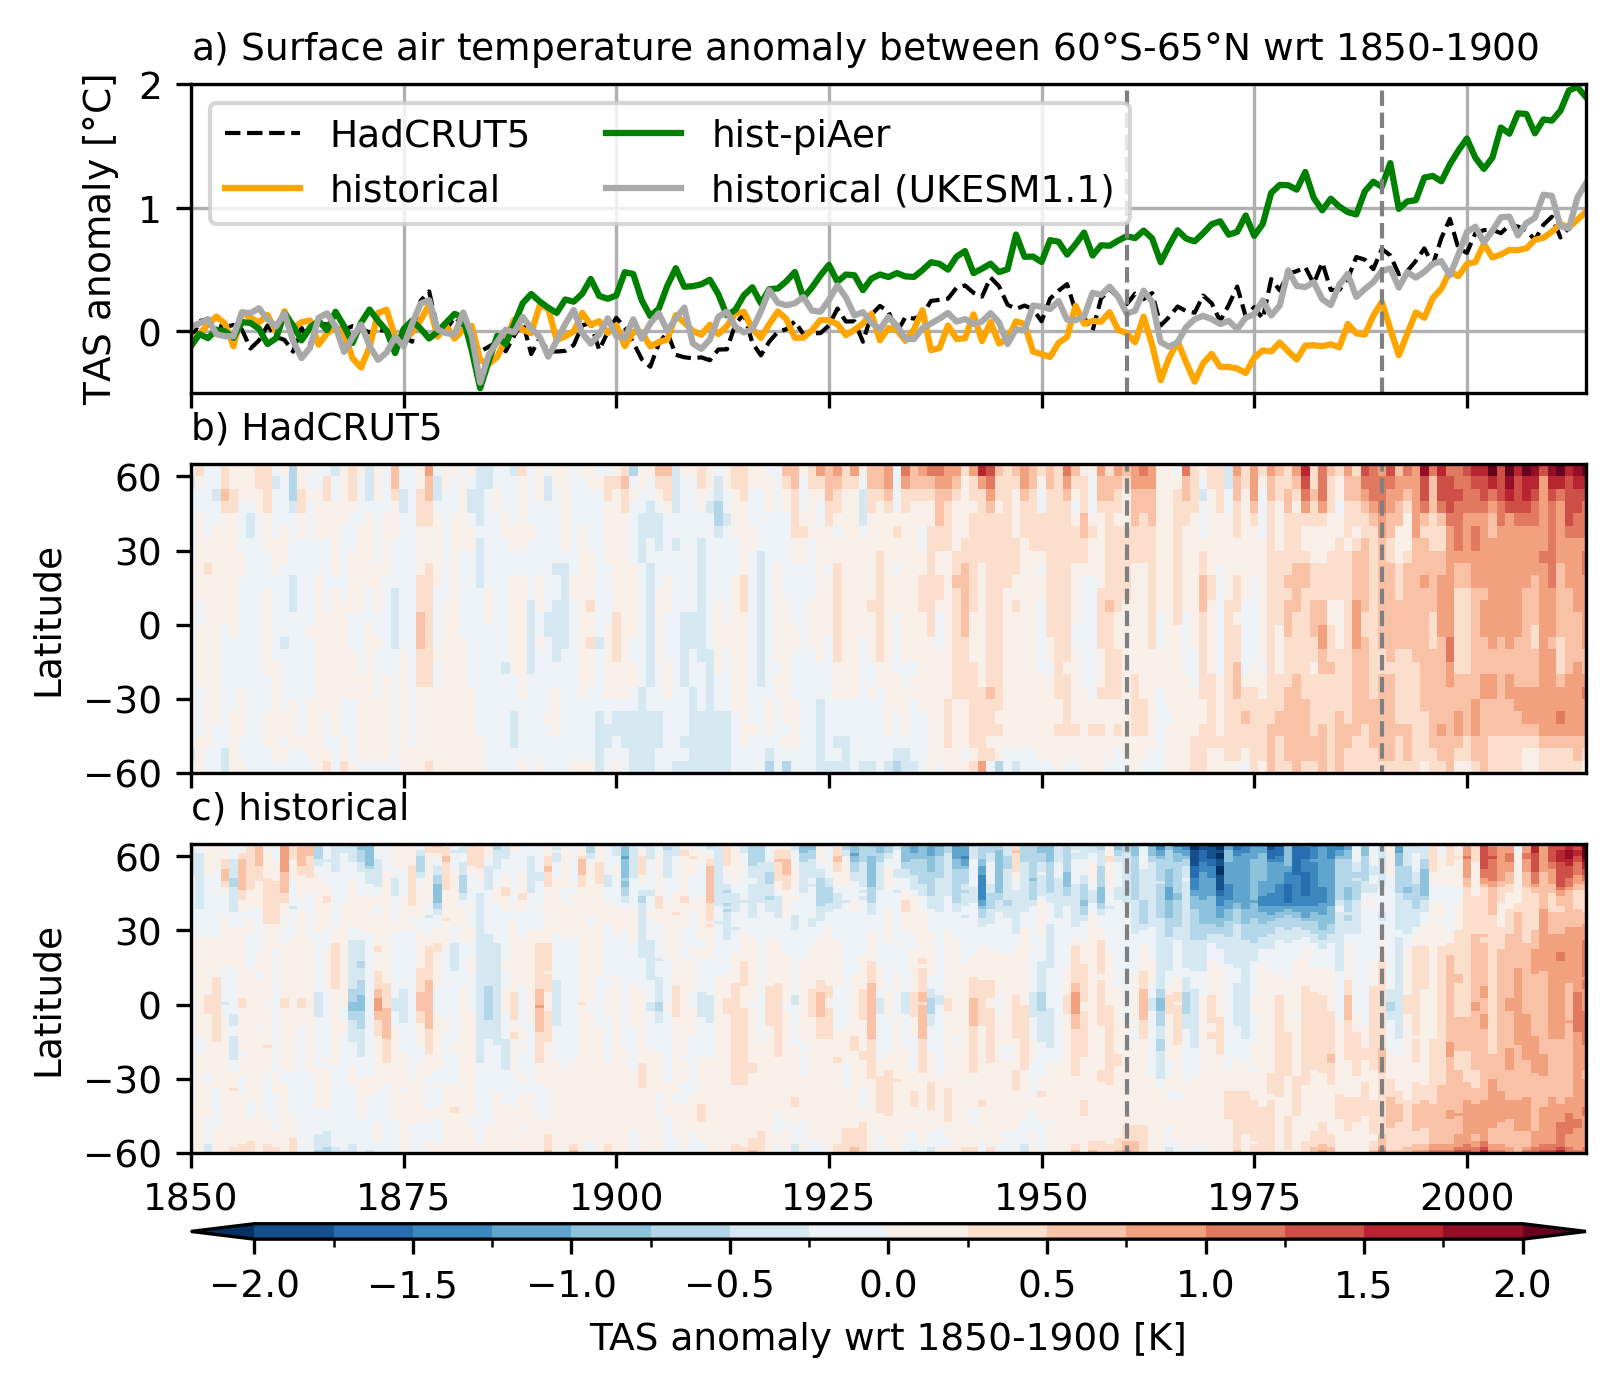
\includegraphics{Chapter4/Figs/TAS_anomaly_cropped.png}
    \caption[Surface air anomaly from HadCRUT5, UKESM1, and UKESM1.1 between 1850 and 2015]{a) Annual mean surface air temperature anomaly between 1850 and 2015 with respect to 1850 to 1859 averaged over latitude 60\textdegree S and 65\textdegree N. b) Surface air temperature anomaly from HadCRUT5 adjusted to 1850--1859. c) surface air temperature from UKESM1 \hist{} simulation. Grey dashed lines are the period between 1960--1989 when the ESMs consistenly underpredict TAS and are called the pothole period.}
    \label{fig:ch4:seasonal-tas-anomaly}
\end{figure}

Figure \ref{fig:ch4:seasonal-tas-anomaly} shows the surface air anomaly from HadCRUT5 and UKESM1.  HadCRUT5 is a gridded dataset of global historical surface temperature anomalies relative to a 1961--1990 reference period. Data are available for each month from January 1850 onwards on a 5 degree grid time series \citep{moriceUpdatedAssessmentSurface2021}. The plot has been readjusted with respect to 1850--1859 climatology to show the temperature evolution and the pothole. Annual mean surface temperature from UKESM1 agrees well with HadCRUT5 both before and after the pothole period with especially cold bias in the Northern Hemisphere. This behaviour is observed amongst other ESMs with varying degree of bias, but not in models with lower complexity. The cause for this behaviour is unclear \citep{zhangRoleAnthropogenicAerosols2021}.

UKESM1 overestimated surface \ce{SO2} concentration which has been thought to related to its dry deposition and cause the pothole cooling \citep{hardacreEvaluationSO2SO422021}. A new version of UKESM1, called UKESM1.1, has recently been released with a higher \ce{SO2} dry deposition to address this challenge \citep{mulcahyUKESM11DevelopmentEvaluation2023}. While the new dry deposition scheme improved the surface air temperature predicton, this has exacerbated the model low bias in \ce{SO4}. Thus, better understanding of chemistry-aerosol-climate interaction is still needed to address the pothole problem.

\subsection{Observed seasonal trend in \ce{SO2} oxidation}
\label{ch4:seasonal-so2-oxidation-observation}

Research on \ce{SO2} primarily focused on its health impacts either as \ce{SO2} gas or contribution to particulate matter \citep[e.g. ][]{meagherSeasonalVariationAtmospheric1983,eatoughConversionSO2Sulfate1994, feichterSimulationTroposphericSulfur1996} \change{ Add this reference https://www.sciencedirect.com/science/article/pii/0004698181902596}. As such, earlier work on \ce{SO2} oxidation has not made the connection between \ce{SO2} oxidation, cloud, and climate until after the work of \citet{twomeyInfluencePollutionShortwave1977} and \citet{albrechtAerosolsCloudMicrophysics1989} on aerosol-cloud feedback has gained traction \change{ add ref on charlson 1991, 1992: https://www.tandfonline.com/doi/abs/10.3402/tellusa.v43i4.11944 https://www.science.org/doi/abs/10.1126/science.255.5043.423  } .  

One of the aspect of \ce{SO2} oxidation that has been observed but not well-studied is the seasonal cycle of the oxidation. Earlier research show that \ce{SO2} conversion rate to sulfate by \ce{SO2 + OH} increases by a factor of 1 between summer and winter \citet{meagherSeasonalVariationAtmospheric1983}. A model study also indicates that the oxidant levels and respective oxidation exhibit a seasonal cycle \citet{feichterSimulationTroposphericSulfur1996}. 

% Evidence that oxidants vary between seasons
According to field studies using instrumented aircraft sampling down-wind air from coal-fired power plants between 1975--1978, the gas-phase \ce{SO2} oxidation has a strong seasonal cycle \citep{meagherSeasonalVariationAtmospheric1983}. The rate of conversion of \ce{SO2} to \ce{SO4^-2} rate varies from a winter low of \qty{1.5E-3}{\per\hour} to a summer high of \qty{1.3E-2}{\per\hour}. 


Conversion rate, $k(\ce{SO4^2-})$, is calculated from
\begin{equation}
k(\ce{SO4^2-}) = \frac{\ce{SO4^2-}]}{([\ce{SO2}]+[\ce{SO4^2-}])t}
\end{equation}
where t is the plume travel time. The plume was sampled at several downwind distances.


In the same study, correlation analysis was also performed between conversion rate and other parameters, including type of power plant and location, time of day, solar intensity, temperature, background \ce{O3} concentration, relative humidity, and specific humidity. Only specific humidity and temperature correlate significantly with the conversion rate. This work suggested that the correlation is due to the seasonal trend rather than a direct relationship of the variable \citep{meagherSeasonalVariationAtmospheric1983}.


% Modelling studies agree with observations
Modelling studies also suggest that there is a 4-fold increase in \ce{SO2 + OH} oxidation between summer and winter which agrees with \ce{SO2} conversion rate at noon at 35 \textdegree N observed as shown in Fig. \ref{fig:ch4:meagher1983} \citep{meagherSeasonalVariationAtmospheric1983}. 

\begin{figure}
    \centering
    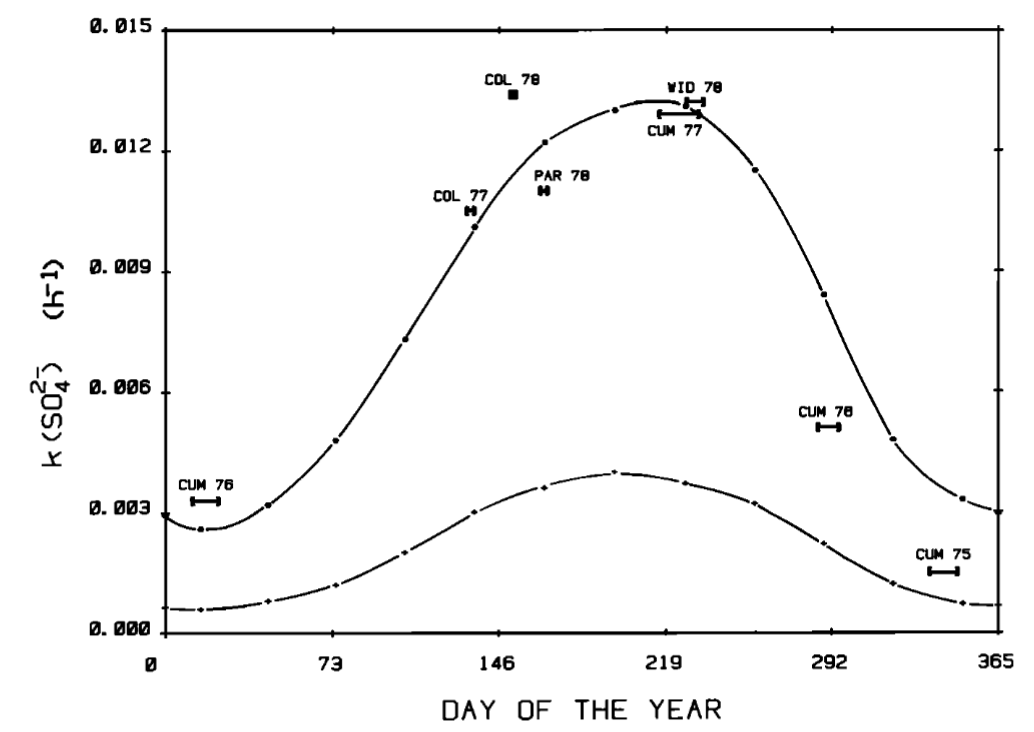
\includegraphics[width=0.8\linewidth]{Chapter4/Figs/meagher1983.png}
    \caption{Average rate of \ce{SO2} conversion to \ce{SO_4^{2-}} measured at different power station plumes. Also shown in this figure are the noontime (top curve) and diurnal average (bottom curve) \cite{meagherSeasonalVariationAtmospheric1983}}
    \label{fig:ch4:meagher1983}
\end{figure}


\ce{SO2 + OH} oxidation is the most important and most rapid during daytime and in summer due to more OH concentration from photochemical reactions \citet{eatoughConversionSO2Sulfate1994}. However, \ce{H2O2} oxidation becomes more important during nighttime or when atmospheric water droplets are present, such as in clouds and fog \cite[e.g. ][]{eatoughConversionSO2Sulfate1994} \change{ Add this reference https://www.sciencedirect.com/science/article/pii/0004698183901816 and https://www.sciencedirect.com/science/article/pii/0004698182903481 and https://agupubs.onlinelibrary.wiley.com/doi/10.1029/91JD01943}. 


Field studies suggest that the aqueous-phase concentration of the oxidant and the reaction kinetics factors, including cloud droplet pH and temperature, are the two important factors influencing the oxidation process \cite{eatoughConversionSO2Sulfate1994}. \ce{SO2} in the gas phase gets dissolved into water droplets along with \ce{O3} and \ce{H2O2}. Both \ce{O3} and \ce{SO2} are moderately soluble in the pH range 3--6, which is the typical atmospheric acidity. Most of the dissolved \ce{SO2} will be present as \ce{HSO3^-} with the concentration of \qty{e-4}{M}. Atmospheric mixing ratio of tropospheric \ce{O3} generally falls in the range between 50-100 ppb, resulting in approximately \num[]{e-9} M. \ce{H2O2} is very soluble, with the atmospheric mixing ratio between 0.1-5 ppb, aqueous concentration is expected at about \qty{e-4}{M} \cite{eatoughConversionSO2Sulfate1994}.


\subsection{Modelling studies showing seasonal trend in \ce{SO2} oxidation and radiative effects}

Most studies in the literature focus on the effects of \ce{SO2} oxidation on air pollution, especially on particulate matter concentration and acid rain \cite[e.g.][]{eatoughConversionSO2Sulfate1994} \change{ Add this reference https://www.sciencedirect.com/science/article/pii/0004698183901816 and https://www.sciencedirect.com/science/article/pii/0004698182903481 and https://agupubs.onlinelibrary.wiley.com/doi/10.1029/91JD01943}. One model study shows a global \ce{SO2} oxidation trend for gas- and aqueous-phase oxidation \cite{feichterSimulationTroposphericSulfur1996}. 

\begin{figure}
    \centering
    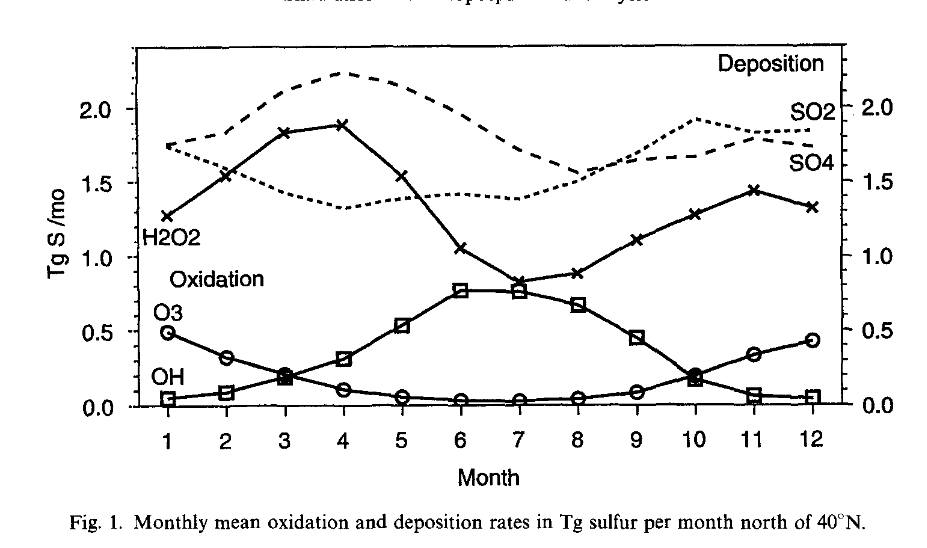
\includegraphics[width=0.8\linewidth]{Chapter4/Figs/feitcher1996.png}
    \caption{Monthly mean \ce{SO2} oxidation and deposition from ECHAM3 \cite{feichterSimulationTroposphericSulfur1996}}
    \label{fig:ch4:feichter1996}
\end{figure}

Figure \ref{fig:ch4:feichter1996} shows the seasonal trend in \ce{SO2} oxidation from general circulation model (CTM) ECHAM3 developed at the Max-Planck Institute for Meteorology. Emission, transport, chemistry and rainout of the sulfur species DMS, S O 2 and sulfate are
calculated on-line with the meteorology in ECMAM3 which offers a high temporal resolution but the spatial resolution is not fine enough to adequately resolve synoptic scale weather patterns. The  model treats DMS and \ce{SO2} as gas, and \ce{SO4^2-} as aerosol, all of which are prognostic variables. During summer months, about half of sulfate aerosols are simulated in cloud and the other half as homogeneous gas-phase reaction. While in winter, most sulfate production occurs in aqueous phase \citep{feichterSimulationTroposphericSulfur1996}.


Recently, seasonal difference of ERF due to aerosols has been quantified \citep{bellouinRegionalSeasonalRadiative2016}. Four models participated in this simulations including three general circulation models: ECHAM6-HAM2, HadGEM3-GLOMAP, NorESM1-M \info{Based on data portal, ECHAM6-1-05-LR, HadGEM2-A/AO/CC/ES, NorESM1-M participated in CMIP5} and one chemical transport model: OsloCTM2. In this study, simulations last one year after spin-up. Emissions from four regions (Europe, East Asia, Rest of the world, and shipping sector) for the year 2008 are reduced by 20\%  to represent feasible emission reduction in two seasons: summer (May--October) and winter (November--April). In case of \ce{SO2} emissions, the perturbations reduce \ce{SO2} emissions by -1.54 and \qty{-1.7}{Tg(S)~yr^{-1}} in Europe, -6.28 and \qty{-6.7}{Tg(S)~yr^{-1}} in East Asia, and -10.2 and \qty{-10.4}{Tg(S)~yr^{-1}} for the rest of the world, in summer and winter, respectively.


\begin{figure}
    \centering
    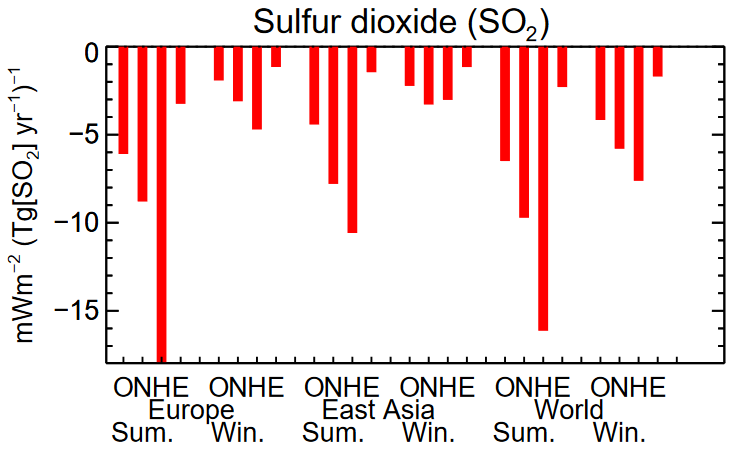
\includegraphics[width=0.5\linewidth]{Chapter4/Figs/bellouin2016.png}
    \caption{ Specific radiative forcing (SRF) given in \unit{(mW~m^{-2})~(Tg(\ce{SO2})~yr^{-1})} for regional and seasonal reduction in \ce{SO2} emissions from four models:  OsloCTM2 (O), NorESM1-M (N), HadGEM3-GLOMAP (H) and ECHAM6-HAM2 (E) \cite{bellouinRegionalSeasonalRadiative2016}}
    \label{fig:ch4:bellouin2016}
\end{figure}

Climate impact of each of the forcing in this studies are normalised by its emission to allow for comparison between emission rates, called the specific RF (SRF), as shown in Figure \ref{fig:ch4:bellouin2016}. HadGEM3-GLOMAP \change{What is the relationship between HadGEM2, HadGEM3-GLOMAP and UKESM1??????? UKESM1 physical model is HadGEM3-GC3.1 but does that mean HadGEM3 is a predecessor to UKESM1??? But Sellar (2019) says  predecessor is HadGEM2-ES......} which is a close relative to UKESM1 shows the largest change in ERF per unit of \ce{SO2} emissions in summer from Europe at \qty{18}{(mW~m^{-2})~(Tg(\ce{SO2})~yr^{-1})} or \qty{0.036}{(W~m^{-2})~(Tg(S)~yr^{-1})}.

Another study compares the sulfur budget across many ESMs, focusing on stratospheric sulfate aerosols \citep{brodowskyAnalysisGlobalAtmospheric2024}. However, there are no discussions on tropospheric sulfate aerosol seasonal trends or seasonal radiative effects.

Despite extensive measurement campaigns in the late 20\textsuperscript{th} century to quantify the changes in \ce{SO2} and its oxidation and recent developments in the radiative effects of aerosols, no studies have linked the seasonality of oxidation to radiative effects.


\subsection{Research opportunities and motivation}

This means \ce{SO2} emission in summer could lead to more aerosol number production compared to winter. As aerosol-cloud interaction depends more strongly on the change in aerosol number, one could hypothesise that the aerosol-cloud interaction would be stronger during summer due to more aerosol numbers. While both measurement and modelling studies have confirmed the seasonal cycle of \ce{SO2} oxidation, there has not been a detailed study of how this change in aerosol formation would affect cloud formation in the historical period. 

UKESM1 simulates both aerosol mass and number independently, making it one of the most robust climate models regarding aerosol simulation. GLOMAP-mode, the aerosol module used in UKESM1, simulates both soluble and insoluble aerosols in four modes: nucleation, Aitken, accumulation, and coarse, and different aerosol types: sulfate, sea salt, organic, dust, and black carbon. It also simulates interaction between modes such as coagulation and condensation and wet and dry deposition. This makes UKESM1 a valuable tool for studying the aerosol properties in different seasons.


\section{Methods and data}

This Chapter examines how \ce{SO2} oxidation in UKESM1 responds to changes in physical and chemical parameters. General information on the model is described in Chapter \ref{ch2:title}.

\subsection{Sulfate production rates in UKESM1}
\label{ch4:sec:so4-prod-rate}

The majority of sulfate aerosols are produced in the atmosphere via oxidation. Approximately 5\% of total sulfate production is from primary emissions, which reflects 2.5\% of anthropogenic \ce{SO2} emissions that are assumed to enter the atmosphere as sulfate aerosols. The other 95\% of sulfate aerosol in UKESM1 are produced in two pathways: gas-phase oxidation of \ce{SO2} and OH, producing sulfuric acid, which nucleates into new particles, and aqueous-phase oxidation in cloud droplets. 

Gas-phase oxidation of \ce{SO2 + OH} is a termolecular reaction, Reaction \ref{ch1:eq:so2-oh}, with the parameters for rate constant given in Table \ref{ch4:tab:so2-oh-reaction-consts} a function of the concentration of air, [M], and temperature, T.
\begin{align}
    \dfrac{d[\ce{SO2}]}{dt} =  k_{([M],T)} [\ce{SO2}][\ce{OH}][\ce{M}] \label{ch4:eq:so2-oh-prod}
\end{align}

The rate constant for the termolecular reaction, $k_{([M],T)}$, is given below.
\begin{align}
    k_0 &= k_1 \left(\frac{T}{300}\right)^{\alpha_1} \exp{(-\beta_1/T)} \label{ch4:eq:so2-oh-k0}\\
    k_\infty &= k_2 \left(\frac{T}{300}\right)^{\alpha_2} \exp{(-\beta_2/T)} \label{ch4:eq:so2-oh-k_inf}\\
    k_{([M],T)} &= \left( \frac{k_0[M]}{1+\frac{k_0[M]}{k_\infty}}\right) F_c^{\left\{ 1+\left[ \log_{10} \left( \frac{k_0[M]}{k_\infty}\right) \right]^2 \right\}^{-1}} \label{ch4:eq:so2-oh-k_MT} 
\end{align}

The free radical \ce{HSO3} reacts in a chain of reactions with \ce{O2} and \ce{H2O} to form \ce{H2SO4}.

\begin{table}[]
\centering
    \begin{tabular}{ccccccccc}
    \hline
    Reactants & Products & $F_c$ & $k_1$ & $\alpha_1$ & $\beta_1$ & $k_2$ & $\alpha_2$ & $\beta_2$ \\ \hline
    \ce{SO2 + OH} & \ce{SO3 + HO2} & 0.60 & 3$\times 10^{-31}$ & -3.3 & 0 & 1.5$\times 10^{-12}$ & 0 & 0 \\ \hline
    \end{tabular}
\caption{constants for \ce{SO2 + OH} reaction}
\label{ch4:tab:so2-oh-reaction-consts}
\end{table}

The aqueous-phase reactions in UKESM1 require information about cloud droplets and cloud droplet acidity as acidity determines rates of \ce{SO2 + O3} and \ce{SO2 + H2O2} reactions \citep{seinfeldAtmosphericChemistryPhysics2016}. Once the reaction rates are determined from Equation \ref{ch1:eq:so2-o3}--\ref{ch1:eq:so2-h2o2}, the in-cloud sulfate aerosol production is obtained from
\begin{align}
    \Delta S_{\mathrm{cloud}} = F \cdot \left( \dfrac{d[S(IV)]}{dt}\right) \cdot L \cdot N_a \cdot \frac{1}{\rho_w} \label{ch4:eq:in-cloud-sulfate-prod}
\end{align}
where $F$ is the cloud fraction, $ \dfrac{d[S(IV)]}{dt}$ is the aqueous-phase reaction rate, $L$ is the cloud liquid water content, $N_a$ is the Avogadro's constant, and $\rho_w$ is the density of water. In the model version used in this work, global cloud pH is set to 4.0 where the local \ce{SO2} mixing ratio exceeds 0.5 ppb, or 5.0 if not.


GLOMAP-mode, the aerosol module simulating aerosol processes in UKESM1, treats aerosol number concentration for each aerosol mode separately with interaction such as coagulation and between modes. The aerosol number for each mode is represented by a log-normal distribution with a geometric mean diameter $\bar{D}$ covering the nucleation ($\bar{D} < 10$ \unit{\nano\metre}), Aitken ($10 \leq \bar{D} < 100$ \unit{\nano\metre}), accumulation ($100 \leq \bar{D} < 1000$ \unit{\nano\metre}), and coarse ($\bar{D} \geq 1000$ \unit{\nano\metre}) mode. The mass concentration of each component, including sulfate, sea salt, black carbon, organic carbon and dust in each mode, is also calculated separately. 


% \subsection{Specific ERF}
% \subsection{Adjusted HadCRUT5}
% \subsection{Seasonal mean surface anomaly}


\subsection{Seasonal cycle of \ce{SO2} emissions}

This Chapter employs the AerChemMIP historical fixed-SST transient simulation results from UKESM1. Both the model and simulation set-up are described in Chapter \ref{ch2:title}. \ce{SO2} emissions follow that of CEDS \citep{HoeslyHistoricalEmissions2017}, which shows the seasonal trends in \ce{SO2} emissions. 

\begin{figure}
    \centering
    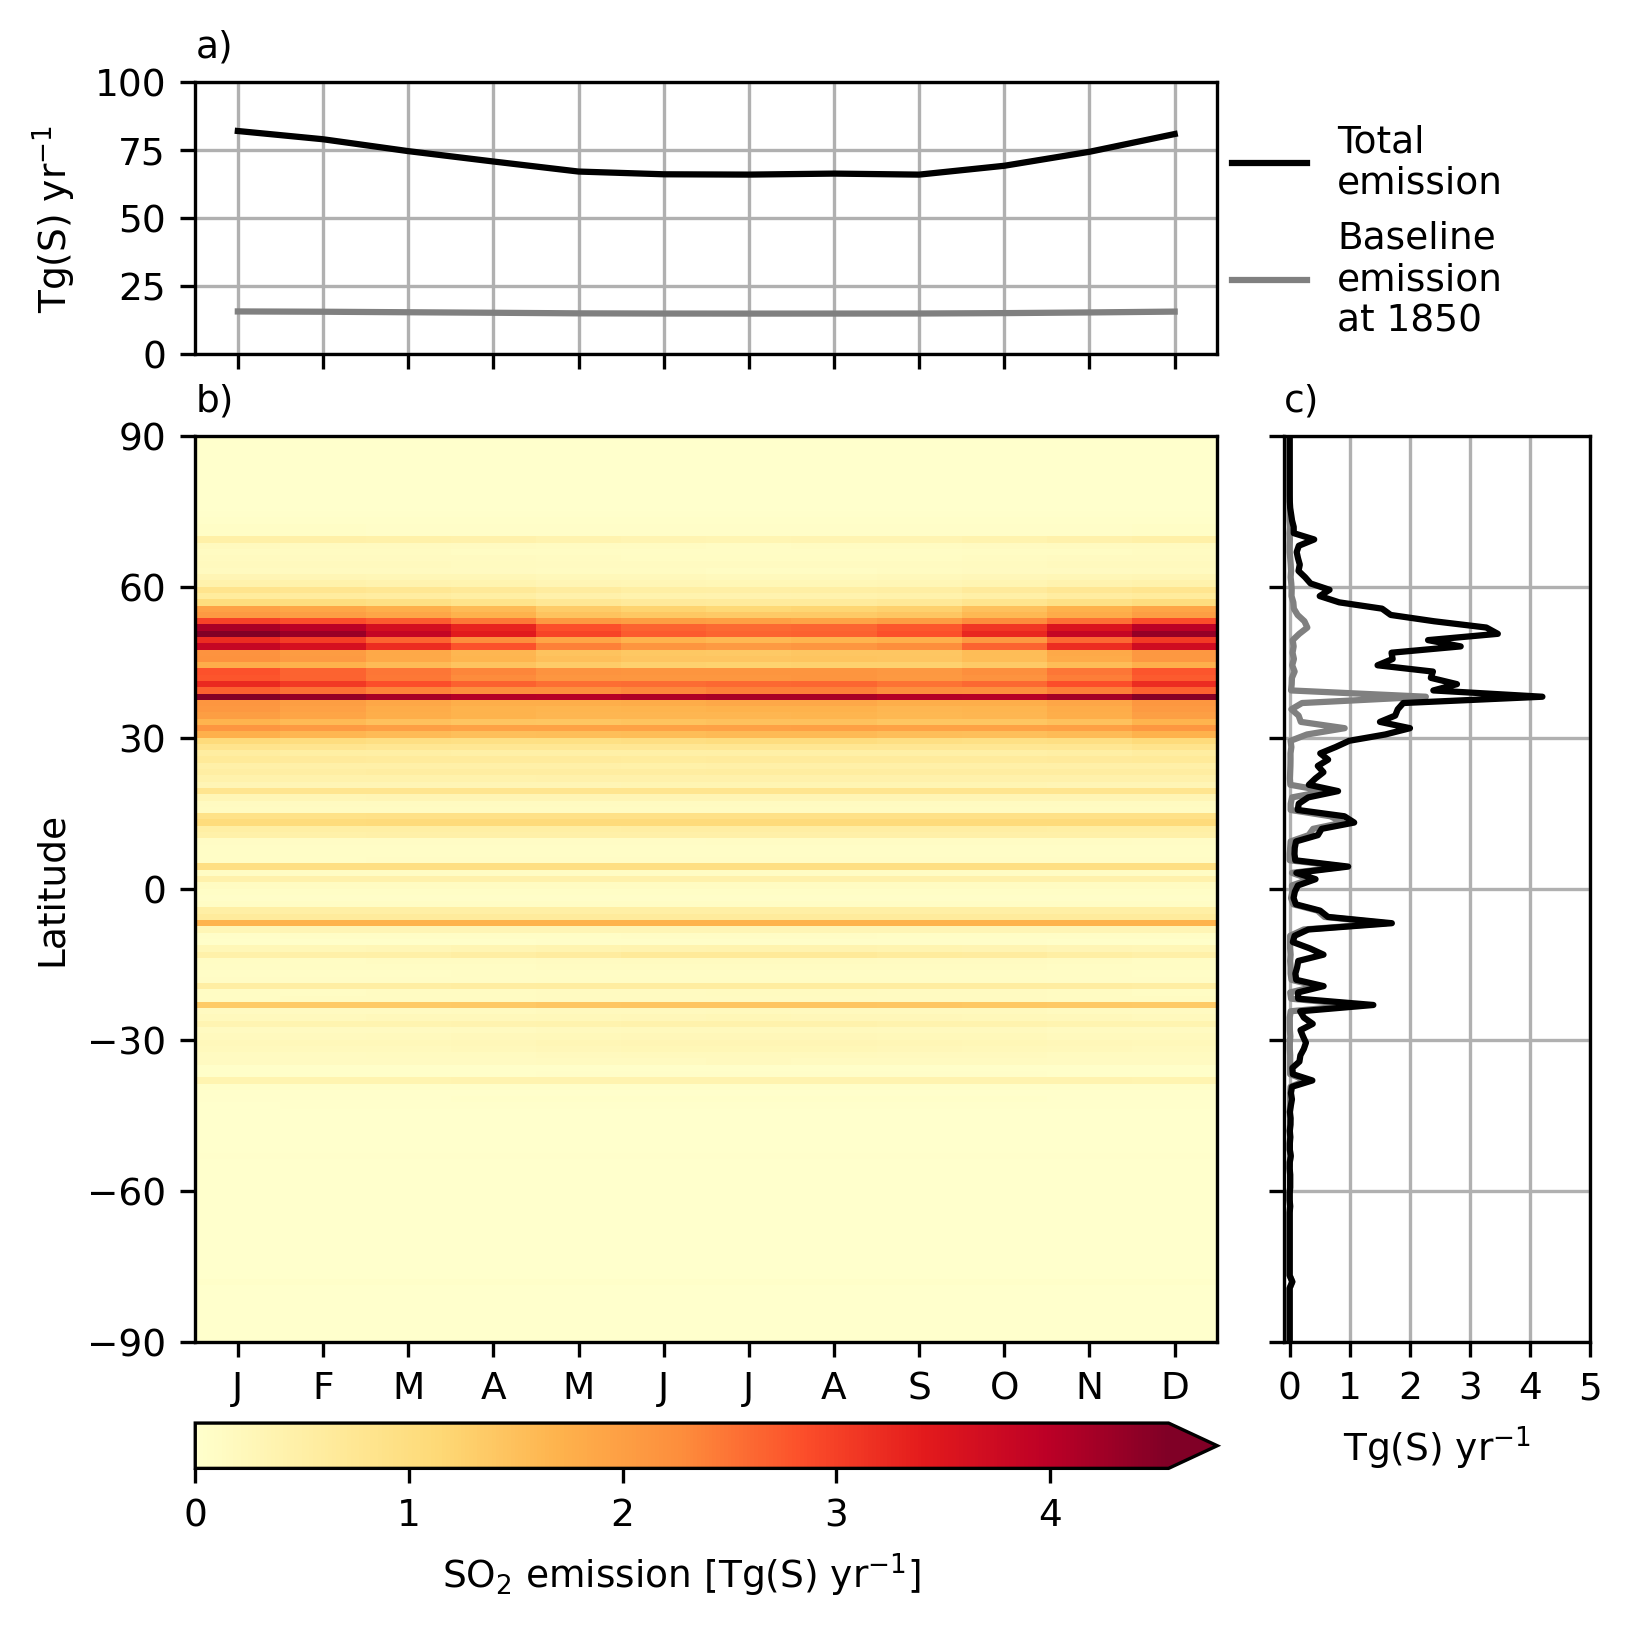
\includegraphics{Chapter4/Figs/emiso2_monthly_pothole.png}
    \caption[Primary \ce{SO2} emissions between 1960 and 1989]{Primary \ce{SO2} emissions between 1960 and 1989. (a) and (c) show total \ce{SO2} emissions from anthropogenic and non-anthropogenic sources at each month and latitude, respectively. (b) shows total emission as a function of month of year and latitude. Baseline emissions are constant and include both anthropogenic and natural emissions.}
    \label{fig:ch4:seasonal-emission}
\end{figure}

Figure \ref{fig:ch4:seasonal-emission} shows primary \ce{SO2} emissions between 1960 and 1989. The anthropogenic emissions rise in the boreal winter as energy usage rises with winter emissions approximately 12.5 \unit{Tg(S)~yr^{-1}} greater than winter's. Most emissions in this period come from fast-growing countries in Europe and North America, accounting for 32.1\% (24.6  \unit{Tg(S)~yr^{-1}}) of the annual mean of 76.6 \unit{Tg(S)~yr^{-1}}. Non-anthropogenic emissions from volcanic degassing contribute to background emissions, which have been constant throughout the years.



\section{Results and discussions}

This Chapter aims to attribute changes in \ce{SO2} oxidation to radiative effects using existing AerChemMIP experiments. The most suitable simulations are the \histsst{} and \sstpiaer, which constrain aerosol precursor emissions at the 1850s level. This poses a challenge for direct attribution as aerosol precursors include not only \ce{SO2} but also precursors for OC and primary BC emissions, making the attribution of changes of \ce{SO2} oxidation to aerosol properties and radiative balance less straightforward. This could be mitigated by selecting suitable periods when \ce{SO2} emissions are significantly greater than OC and BCs. 

A decade between 1960 and 1989 inclusive has been identified for analysis in this Chapter for its high \ce{SO2} emissions and relatively low BC and OC emissions from the main emitting regions: Europe and North America \citep{hoeslyHistorical175020142018}. This period also coincides with the anomalous cooling period. Another period of interest is the near present (2005--2015) when \ce{SO2} emissions increase in Eastern and Southern Asia regions. 

A significant outcome of this Chapter is how changes in seasonal oxidation may modulate the radiative effects of \ce{SO2} emissions with possible effects on the seasonal cycle of surface temperature anomaly. The following needs to be considered when considering the seasonal ERF: the annual cycle of oxidants, sulfate oxidation tendencies, aerosol and cloud properties. The seasonal cycle of ERF and the correlation between oxidation tendencies and aerosol properties are discussed, and changes in ERF per unit of \ce{SO2} emission are quantified. Lastly, this Chapter discusses the correlation between observed seasonal trends in surface temperature anomaly, specifically during the pothole period, and the contribution to temperature changes from aerosols.

\subsection{Seasonal cycle of oxidants}

OH, \ce{O3} and \ce{H2O2} form photochemically in the atmosphere and are involved in oxidising \ce{SO2}. Figure \ref{fig:ch4:seasonal-oxidants} shows global mean oxidant concentrations below 5 km. All oxidants' concentrations strongly correlate to insolation, where maximum concentration follows the solar radiation peaks. \ce{SO2} concentration localises near emission sources and peaks in winter when emissions are more substantial, as shown in Figure \ref{fig:ch4:seasonal-emission}.

\begin{figure}
    \centering
    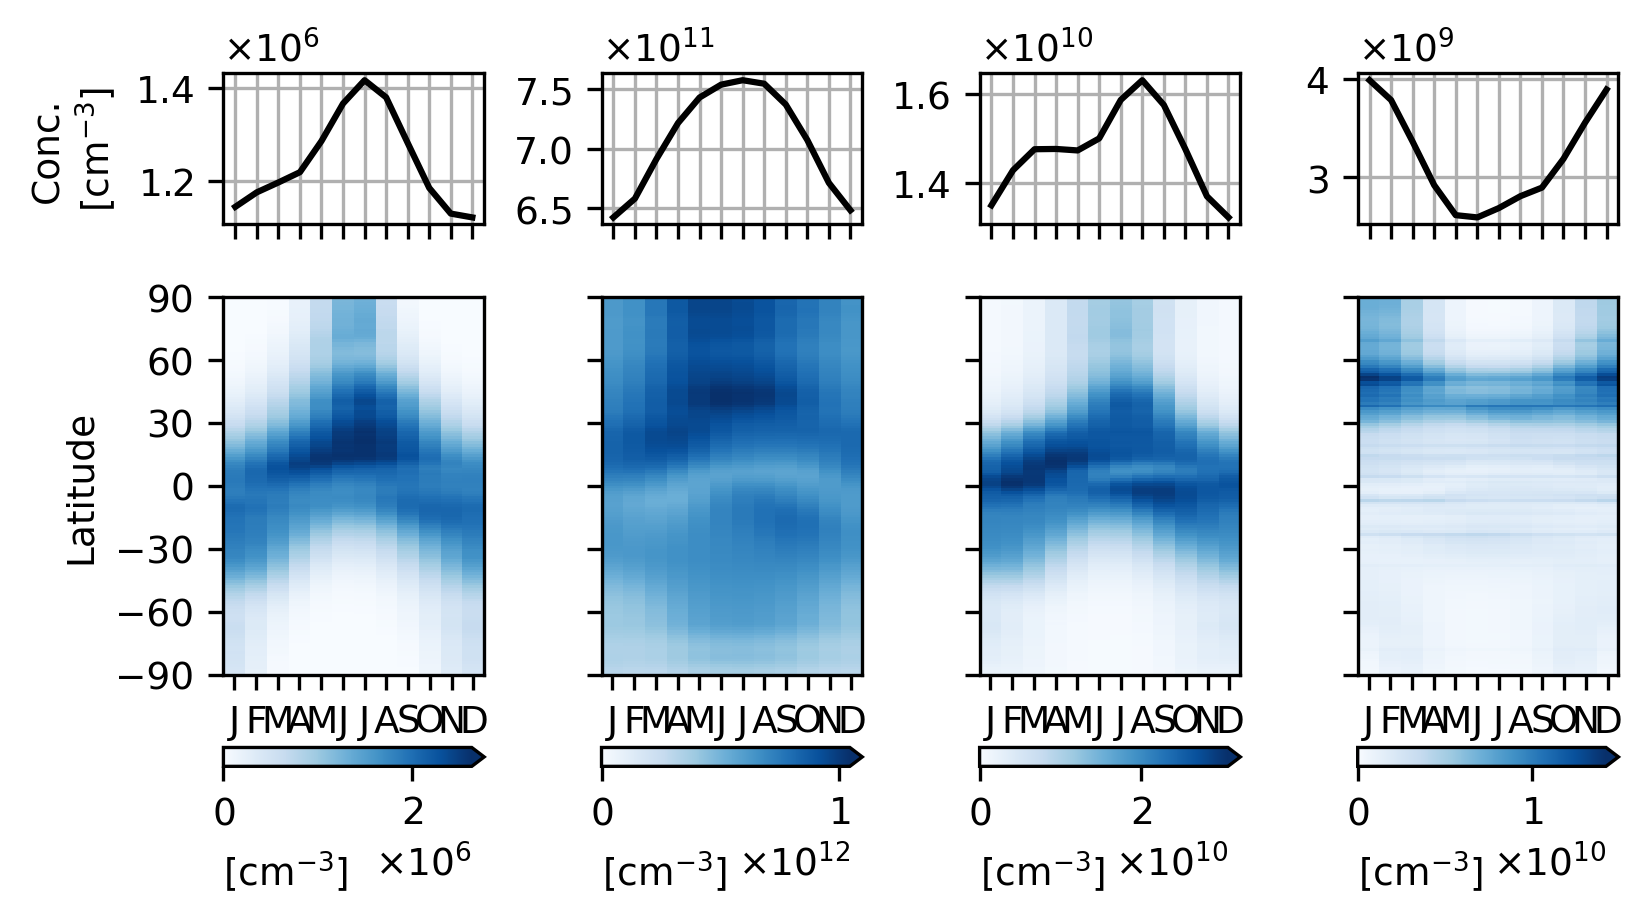
\includegraphics{Chapter4/Figs/seasonal_oxidant_pothole.png}
    \caption[Mean concentration of \ce{OH}, \ce{O3}, \ce{H2O2}, and \ce{SO2} from surface to 5 km between 1960 and 1989]{Global mean concentration of (a) \ce{OH}, (b) \ce{O3}, (c), \ce{H2O2}, and (d) \ce{SO2} from surface to 5 km between 1960 and 1989 as a function of month of year. (e-g) show the respective oxidant concentration as a function of month of year and latitude for the same domain.}
    \label{fig:ch4:seasonal-oxidants}
\end{figure}

Between latitude 30 and 60 \textdegree N where most anthropogenic \ce{SO2} are emitted, OH and \ce{H2O2} concentrations vary greatly between seasons, with their summer concentrations one and two orders of magnitude greater than their respective winter concentrations. OH concentration increases from \num{2.4e5} to \qty{2.1e6}{\per\cubic\cm} and \ce{H2O2} concentration increases from \num{3.0e8} to \qty{2.3e10}{\per\cubic\cm}, as shown in Figure \ref{fig:app1:seasonal-oxidant-30-60}). 

While \ce{O3} concentration between latitude 30 and 60 \textdegree N is also greatest in the boreal summer months, exceeding \qty{1.1e12}{\per\cubic\cm}, its variation is not as drastic, with winter concentration over the same latitude band approximately half that of summer (\qty{7.2e11}{\per\cubic\cm}).

% Discuss SO2 loss via reaction with all the oxidants and refer to the emission seasonal cycle
\ce{SO2} concentration mimics its emission, reaching maximum in winter and minimum in summer. In summer, less \ce{SO2} is emitted, and more is oxidised, leading to a lower concentration and shorter lifetime in summer, discussed in the following section.

\subsection{Seasonal cycle of oxidation}

\begin{figure}
    \centering
    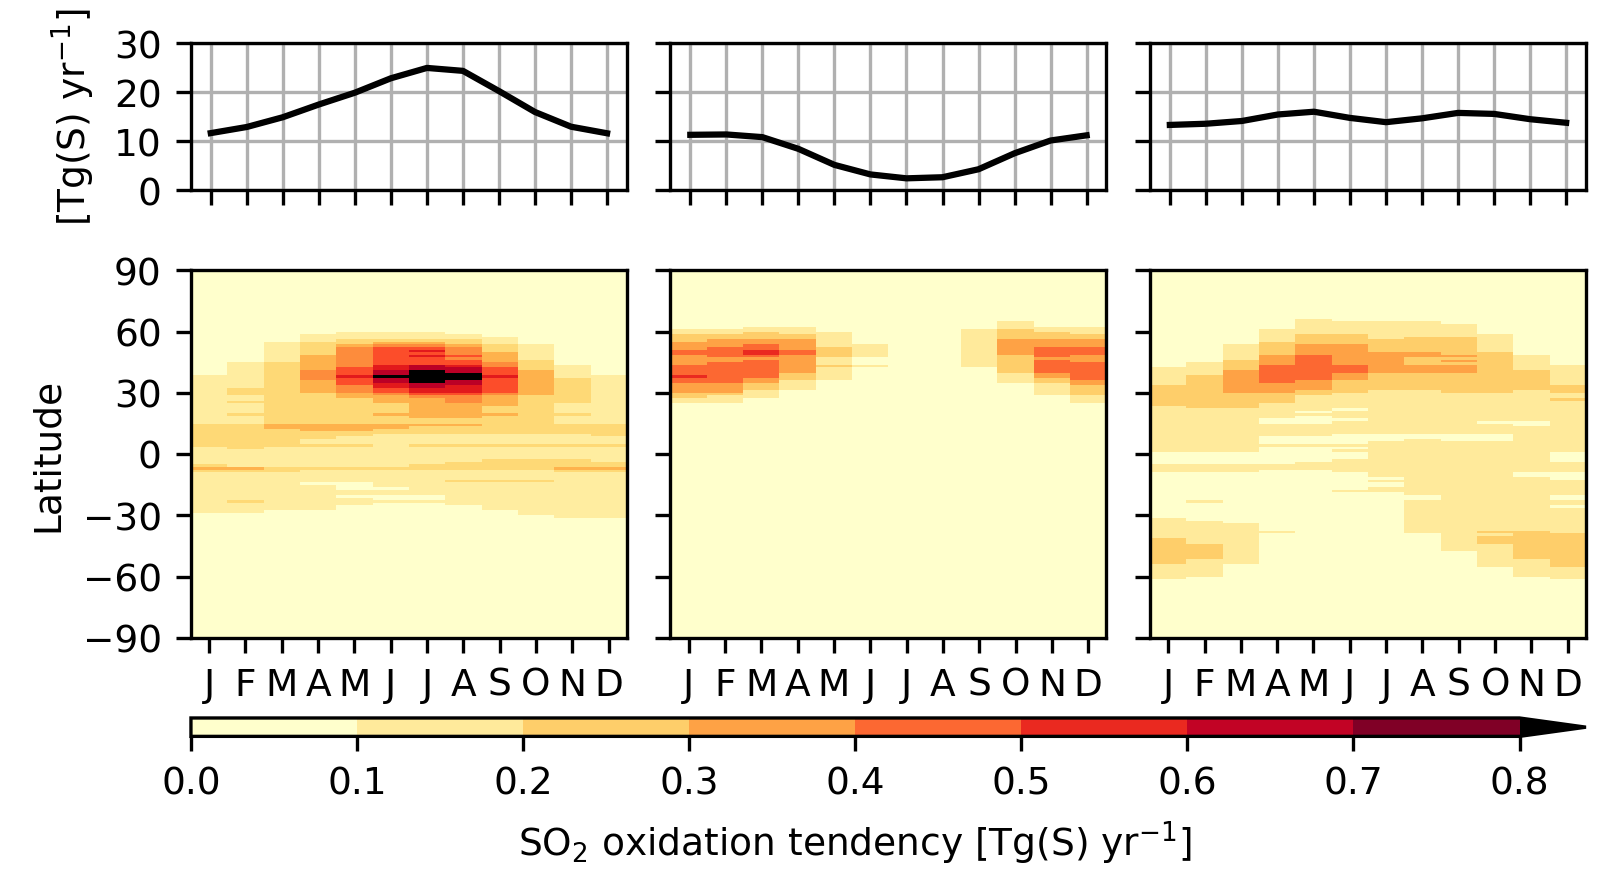
\includegraphics{Chapter4/Figs/seasonal_oxidation_w_summary_histsst_pothole.png}
    \caption[Total tropospheric \ce{SO2} oxidation tendencies as a function of latitude and months between 1960 and 1989]{Total \ce{SO2} oxidation with (a) OH, (b) \ce{O3}, and (c) \ce{H2O2} as a function of months between 1960 and 1989. (d-f) show the respective oxidation tendencies as a function of months and latitude for the same domain.}
    \label{fig:ch4:seasonal-oxidation}
\end{figure}

Figure \ref{fig:ch4:seasonal-oxidation} shows that \ce{SO2 + OH} maximises during boreal summer with a tendency reaching 29 \unit{Tg(S)~yr^{-1}}. This is expected as OH concentration is also high during the same period. However, for aqueous-phase reactions, \ce{SO2 + O3} and \ce{SO2 + H2O2}, the oxidation tendencies do not follow the trends of their respective oxidants. This implies that the concentration levels of \ce{O3} and \ce{H2O2} are not the limiting factor for aqueous-phase oxidation. 

The main difference between gas- and aqueous-phase oxidation lies in their parameterisation. Unlike gas-phase reactions, both \ce{SO2 + O3} and \ce{SO2 + H2O2} take place in cloud droplets. Aqueous-phase oxidation of \ce{SO2} with \ce{O3} and \ce{H2O2} is parameterised in  UKESM1 using Equation \ref{ch4:eq:in-cloud-sulfate-prod}. Multiple processes control the sulfate production rates, each with its limiting parameters. First, the gaseous oxidants dissolve into cloud droplets. This process is limited by the oxidants' Henry's coefficients and their concentrations. The dissolved oxidants react according to reaction rates that depend on the cloud droplet's temperature, pressure, and pH. The amount of available cloud droplets also controls the sulfate production rate as it determines the amount of water in each model grid.

\begin{figure}
    \centering
    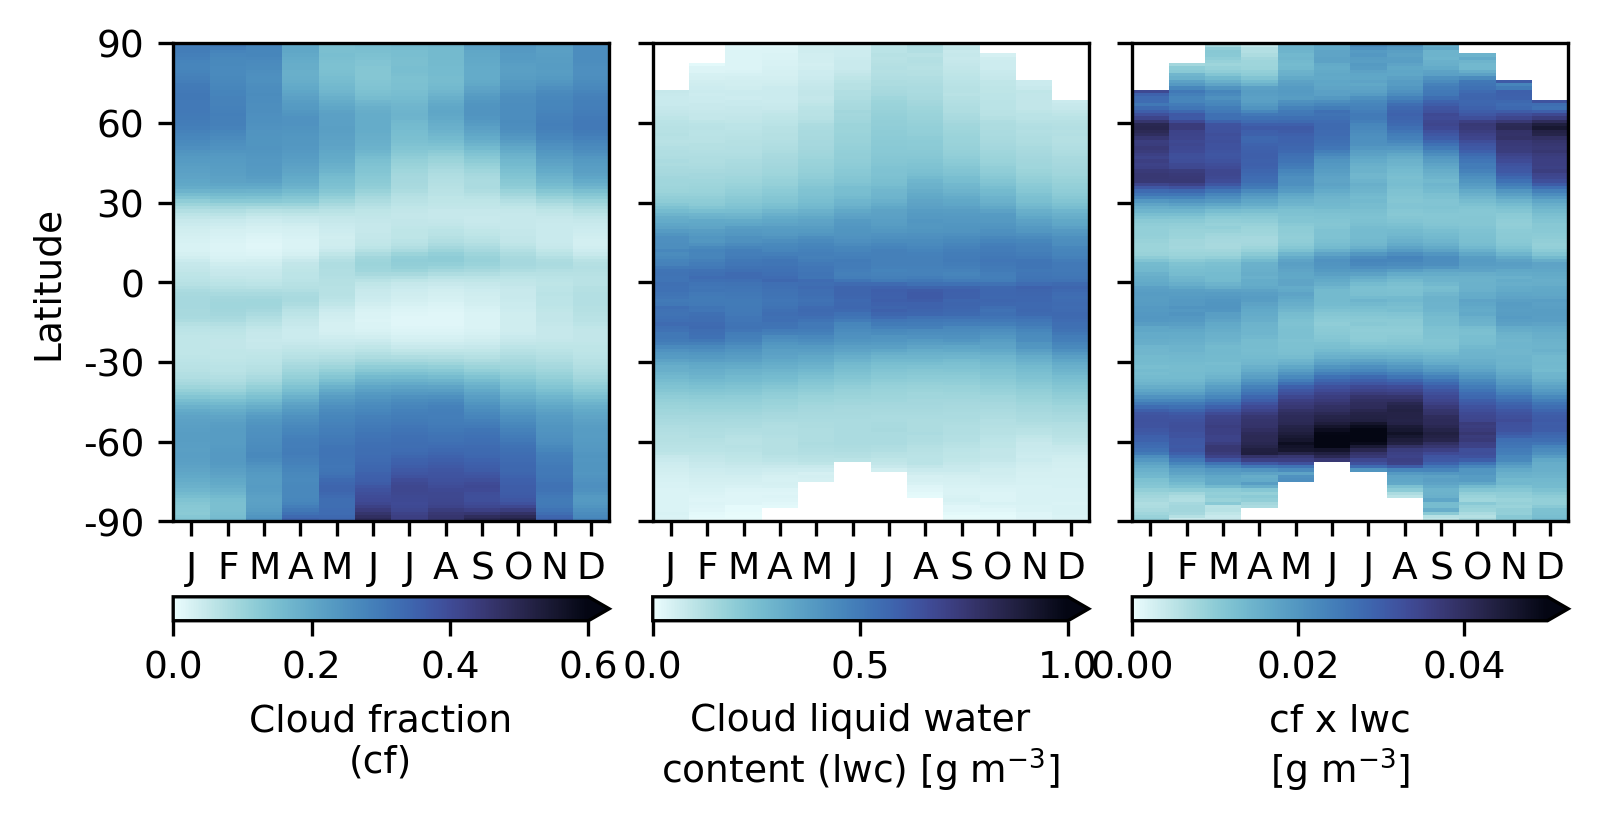
\includegraphics{Chapter4/Figs/seasonal_cf_lwc_histsst_pothole.png}
    \caption[Mean cloud fraction and liquid water content below 10 km between 1960 and 1989]{Mean (a) cloud fraction, (b) liquid water content and (c) products of cloud fraction and liquid water content as a function of latitude and month of the year from the surface up to 10 km between 1960 and 1989.}
    \label{fig:ch4:seasonal-cf-lwc}
\end{figure}

% Define cf and lwc
Cloud processes parameterisation is needed to simulate cloud in Earth System models with coarse grids. Cloud fraction, sometimes referred to as cloud cover, is a parameter which represents the fraction of the total volume of the model grid box that contains any cloud. It is unitless with a value between zero and one. Cloud liquid water content describes the mass of liquid water in a unit volume of air and has the unit of \unit{\gram\per\cubic\metre}.

Both cloud fraction and cloud liquid water content play essential roles in sulfate production in the aqueous phase, enabling the dissolution of gaseous oxidants into cloud droplets. Figure \ref{fig:ch4:seasonal-cf-lwc} shows seasonal trends of both parameters and their products as a function of months and latitude. Higher cloud fraction collocates with lower liquid water content in the mid-latitudes. The products of cloud fraction and liquid water content are greater than \qty{0.03}{\gram\per\cubic\metre} except for summer for mid-latitude, which explains the lower aqueous-phase reaction during the same season. 

The following sub-section explores the theoretical range of all oxidation pathways due to variations in temperature, cloud droplet pH, and cloud fraction to confirm the modelled observation.

\subsubsection{Theoretical range of \ce{SO2} oxidation reaction rates}

In this section, I quantify the factors that limit sulfate production rates in summer and winter conditions by calculating the rates from equations in UKESM1 using parameter values from observation or model averages. 

The equations describing sulfate production includes Equation \ref{ch4:eq:so2-oh-prod}--\ref{ch4:eq:so2-oh-k_MT} for gas-phase reactions, and Equation \ref{ch1:eq:Henry-eq}--\ref{ch1:eq:aq-conc} and \ref{ch4:eq:in-cloud-sulfate-prod} for aqueous-phase reactions. The parameters needed for the gas-phase reaction include concentration of OH and \ce{SO2}, atmospheric temperature and pressure. Aqueous-phase productions by \ce{O3} and \ce{H2O2} are more complex and require cloud parameters, including cloud fraction, liquid water content and cloud pH, in addition to oxidant concentrations, atmospheric temperature and pressure. 


\begin{figure}
    \centering
    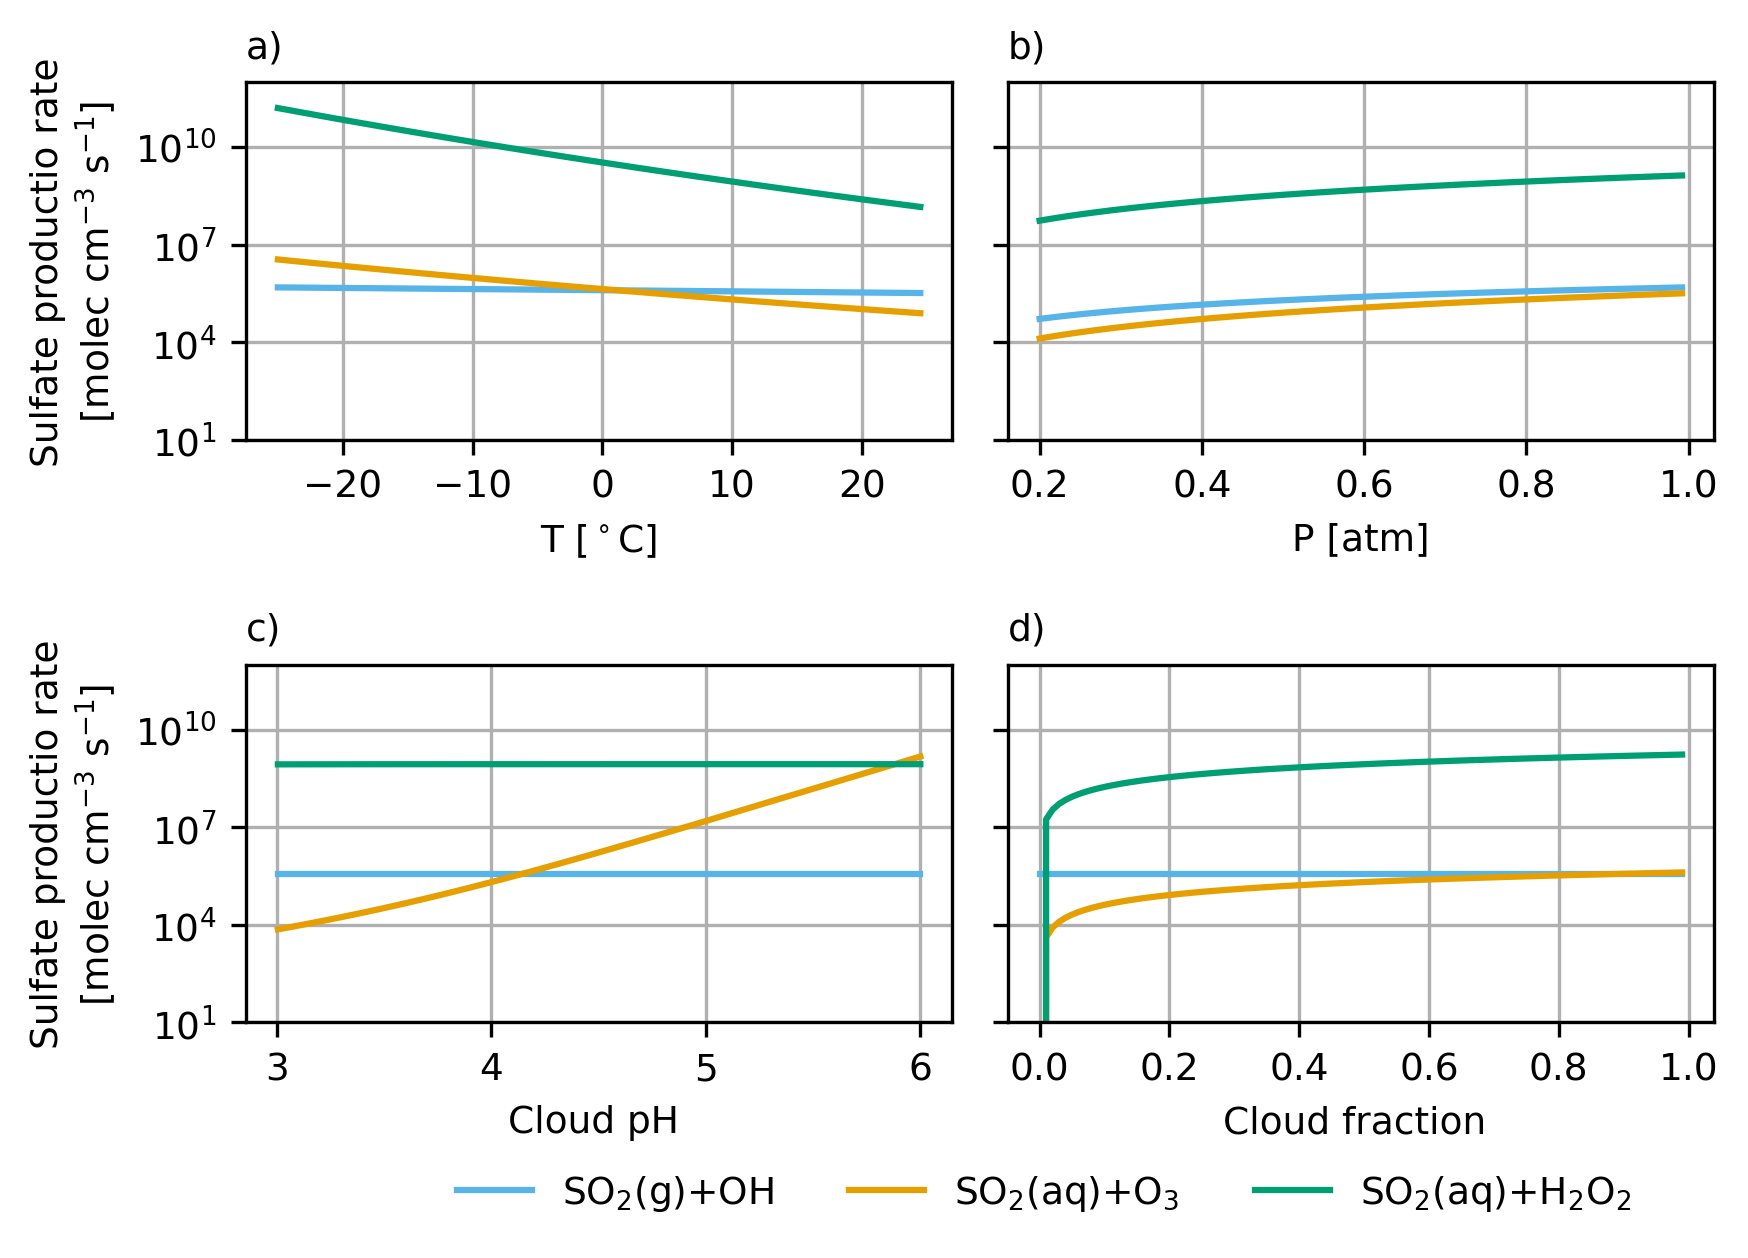
\includegraphics{Chapter4/Figs/oxidation_sensitivity.png}
    \caption[\ce{SO2} oxidation range]{\ce{SO4} production rates for a range of a) atmospheric temperature, b) pressure, c) cloud pH and d) cloud fraction when other parameters are set to average values shown in the first three rows in Table \ref{ch4:tab:sensitivity-test}.}
    \label{fig:ch4:oxidation-sensitivity}
\end{figure}

Changes in sulfate production rates due to temperature, pressure, cloud pH and cloud fraction are shown in Figure \ref{ch4:tab:sensitivity-test}. \ce{SO2 + O3} produces sulfate faster than \ce{SO2 + OH} when the temperature drops below zero \textdegree C, a condition more common in winter and at higher altitudes. Cloud pH strongly influences \ce{SO2 + O3}. \ce{SO2 + O3} oxidation is slower than all other reactions by approximately one order of magnitude except when cloud pH equals 6.0. In this case, \ce{SO2 + O3} reaction rate is the same magnitude as \ce{SO2 + H2O2}. However, this pH is not present in UKESM1 as cloud pH is set to 4.0 or 5.0, depending on the concentration of \ce{SO2}. This thus limits the importance of \ce{SO2 + O3}. Cloud properties do not affect \ce{SO2 + OH} since it is a gas-phase reaction, whereas the aqueous-phase reactions are strongly dependent on cloud fractions, especially when the cloud fraction is below 0.1. 


\begin{table}[]
\centering
\begin{tabular}{p{1.8cm} p{1cm} p{1.25cm} p{1cm} p{1cm} p{0.8cm} p{1cm} p{1cm} p{1cm} p{1cm}}
\toprule
 & \ce{SO2} [ppb] & OH conc. [cm$^{-3}$] & \ce{O3} [ppb] & \ce{H2O2} [ppb] & pH & T [\textdegree C] & P [atm] & CF & LWC [kg m$^{-3}$] \\ \midrule
Average value & 20.0 & 1.0$\times 10^{6} $ & 40.0 & 2.0 & 4.0 & 10.0 & 0.8 & 0.5 & 0.0002 \\
% Minimum & 5.0 & 1.0$\times 10^{5} $ & 20.0 & 0.2 & 3.0 & -25.0 & 0.2 & 0.01 & 0.0002 \\
% Maximum & 50.0 & 5.0$\times 10^{7} $ & 120.0 & 4.6 & 6.0 & 25.0 & 1.0 & 1.0 & 0.0002 \\ 
\midrule
Summer average & 5.0 & 1.0$\times 10^{6} $ & 60.0 & 2.0 & 4.0 & 15.0 & 0.8 & 0.01 & 0.0002 \\
Summer daytime & 20.0 & 5.0$\times 10^{7} $ & 110.0 & 4.6 & 4.0 & 25.0 & 0.8 & 0.01 & 0.0002 \\
Summer nighttime & 10.0 & 3.0$\times 10^{5} $ & 40.0 & 0.1 & 4.0 & 10.0 & 0.8 & 0.01 & 0.0002 \\ \midrule
Winter average & 50.0 & 5.0$\times 10^{5} $ & 30.0 & 1.0 & 4.0 & 0.0 & 0.8 & 0.5 & 0.0002 \\
Winter daytime & 70.0 & 1.0$\times 10^{6} $ & 55.0 & 2.4 & 4.0 & 5.0 & 0.8 & 0.5 & 0.0002 \\
Winter nighttime & 20.0 & 1.0$\times 10^{5} $ & 20.0 & 0.1 & 4.0 & -5.0 & 0.8 & 0.5 & 0.0002 \\ \midrule
Annual average & 20.0 & 1.0$\times 10^{6} $ & 30.0 & 1.0 & 4.0 & 10.0 & 0.8 & 0.1 & 0.0002 \\
Annual daytime average & 20.0 & 1.0$\times 10^{7} $ & 60.0 & 2.0 & 4.0 & 15.0 & 0.8 & 0.1 & 0.0002 \\
Annual nighttime average & 20.0 & 1.0$\times 10^{5} $ & 20.0 & 0.1 & 4.0 & 5.0 & 0.8 & 0.1 & 0.0002 \\ \midrule
UKESM1 summer & 0.1 & 1.4$\times 10^{6} $ & 37.6 & 0.8 & 4.0 & 10.0 & 0.8 & 0.01 & 0.0002 \\
UKESM1 winter & 0.2 & 1.1$\times 10^{6} $ & 31.3 & 0.7 & 4.0 & 10.0 & 0.8 & 0.5 & 0.0002 \\
UKESM1 annual average & 0.2 & 1.3$\times 10^{6} $ & 34.4 & 0.8 & 4.0 & 10.0 & 0.8 & 0.1 & 0.0002 \\ \bottomrule
\end{tabular}
\caption[Parameters for oxidation rates]{Parameters for oxidation rate. CF is cloud fraction, and LWC is liquid water content. Summer, winter, and annual daytime and nighttime averages are taken from field campaigns with similar characteristics (urban areas) where possible. UKESM1 data are taken from Figure \ref{fig:ch4:seasonal-oxidants}, which are monthly mean values.}
\label{ch4:tab:sensitivity-test}
\end{table}


% Describe the oxidant values from different measurement campaigns
The ranges of the sulfate production rates in summer and winter are calculated using oxidant concentrations from different measurement campaigns listed in Table \ref{ch4:tab:sensitivity-test}. \ce{SO2} concentrations are from an urban area in Beijing, China \citep{linCharacteristicsRecentTrends2012}. OH concentrations are taken from two measurement campaigns to cover nighttime and daytime from an urban site in Birmingham, UK \citep{heardHighLevelsHydroxyl2004, khanNighttimeNO3OH2008}. \ce{H2O2} concentrations are taken from rural measurements in Guangzhou, China \citep{huaAtmosphericHydrogenPeroxide2008}. The cloud pH is set to 4.0 as the aerosol module in UKESM1 uses a cloud pH of 4.0 when the concentration of \ce{SO2} is greater than 0.5 ppb \citep{mannDescriptionEvaluationGLOMAPmode2010}. Pressure, cloud fraction and liquid water content are treated as constants.

\begin{figure}
    \centering
    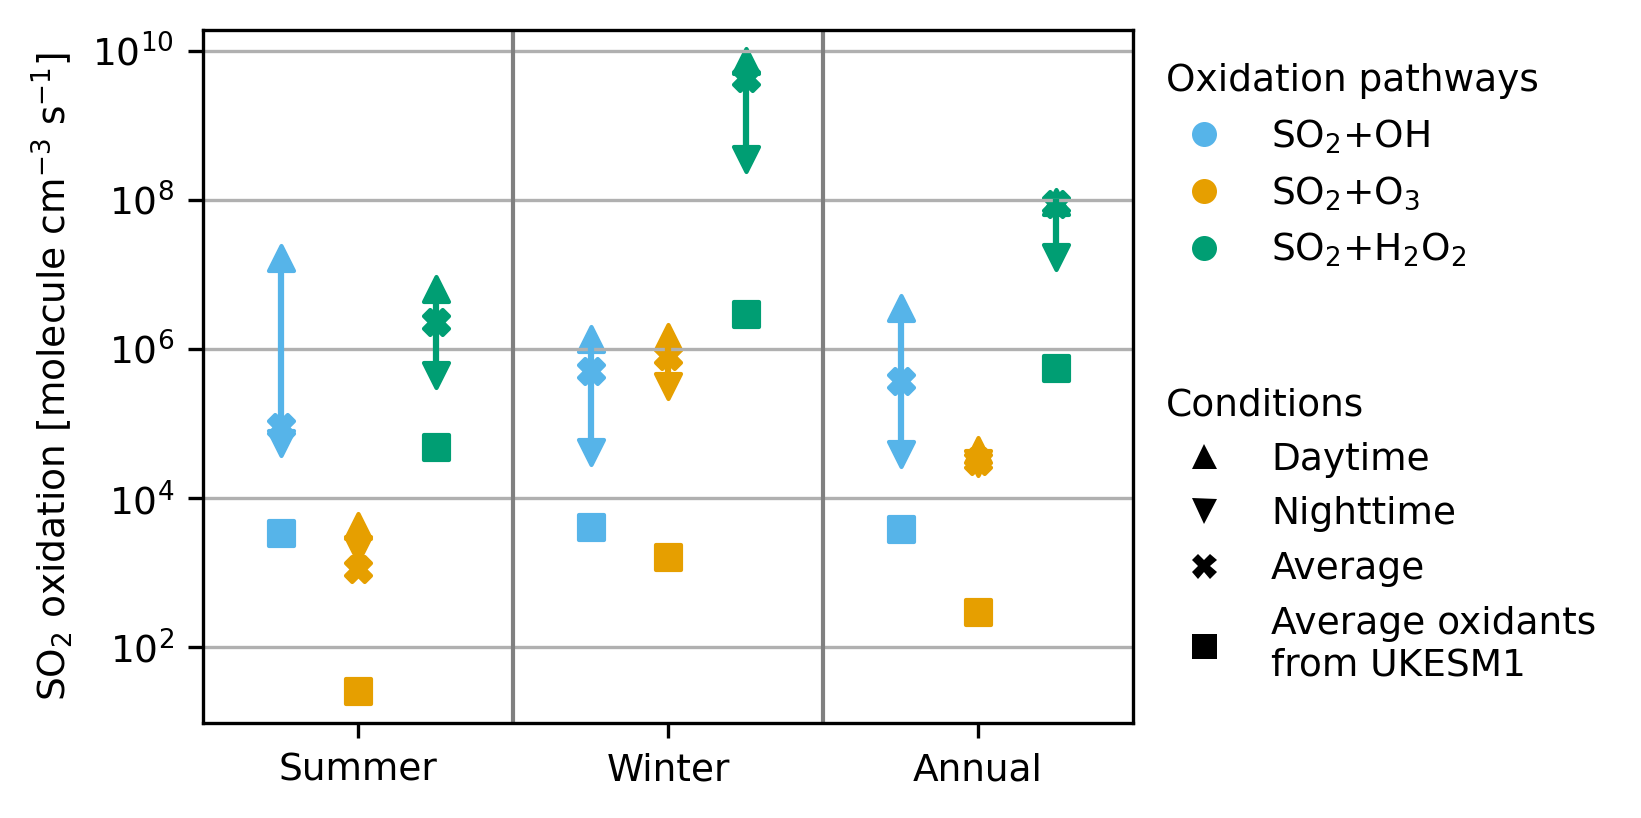
\includegraphics{Chapter4/Figs/theoretical_oxidation.png}
    \caption[\ce{SO4} production rates calculated for summer, winter, and average conditions]{\ce{SO4} production rates calculated for summer, winter, and average conditions as given in Table \ref{ch4:tab:sensitivity-test}.}
    \label{fig:ch4:sensitivity-summary}
\end{figure}

% Explain summer trends for OH
Figure \ref{fig:ch4:oxidation-sensitivity} shows the range of \ce{SO2} oxidation reaction rate in summer and winter using conditions from Table \ref{ch4:tab:sensitivity-test}. \ce{SO2 + OH} is the greatest of all pathways in summer when the temperature and OH concentration are high while the cloud fraction is low. Oxidation by \ce{O3} is the weakest due to low cloud fraction and high temperature. \ce{SO2 + OH} is lower in winter due to lower OH concentration while temperature has negligible effects, as shown in Figure \ref{fig:ch4:oxidation-sensitivity}. 

In contrast, aqueous-phase production by \ce{O3} and \ce{H2O2} increases by two orders of magnitudes in winter compared to summer conditions, placing \ce{SO2 + O3} in the same order of magnitude of \ce{SO2 + OH}. This increase in aqueous-phase production in winter comes from more significant cloud fractions. 

% Comment and compare to other seasonal studies, especially those referenced in the introduction
Comment and compare to other seasonal studies, especially those referenced in the introduction.

The relationship between cloud fraction and aqueous-phase production rate explains the seasonal trends observed in Figure \ref{fig:ch4:seasonal-oxidation}. These results illustrate that cloud property improves aerosol-cloud-climate interaction in UKESM1 and other ESMs. 


\subsection{Sulfur budgets by season}

Oxidation is not the only process that influences the amount of aerosol in the atmosphere. \ce{SO2} may be removed by deposition before it is oxidised into \ce{SO4}. Once oxidised, \ce{SO4} also undergoes deposition, removing it from the atmosphere. All loss processes play a part in determining the lifetime of both sulfur species. This section explores the importance of deposition in determining the sulfur budget and its variation over the year.


\begin{figure}
    \centering
    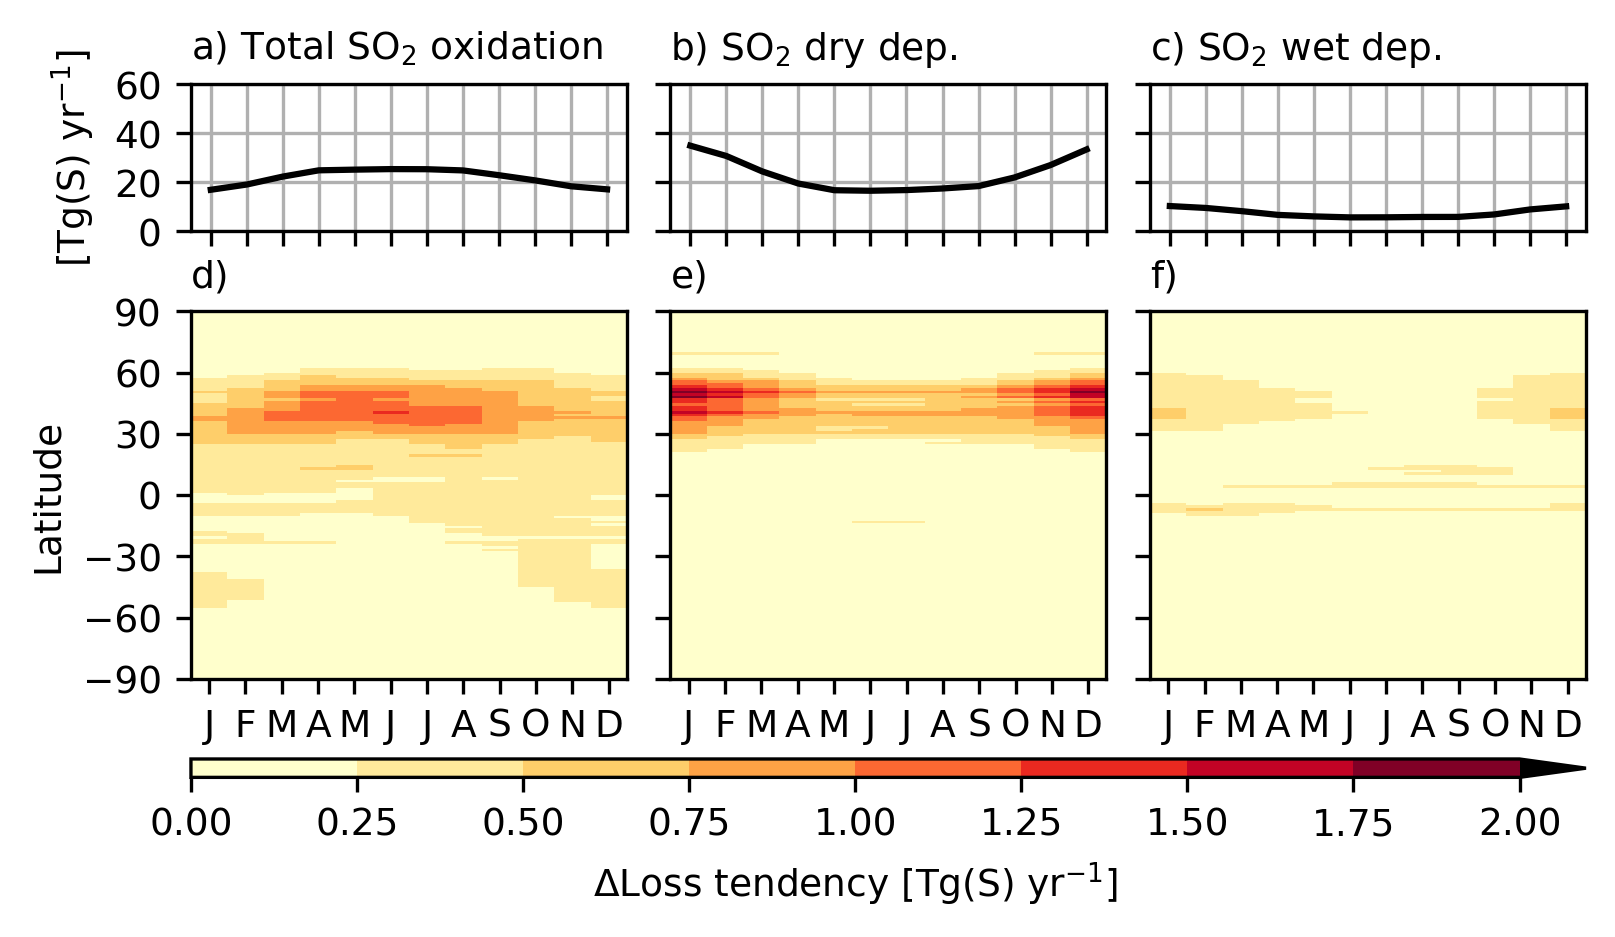
\includegraphics{Chapter4/Figs/so2_losses_histsst_pothole.png}
    \caption[\ce{SO2} loss tendencies due to oxidation and deposition by months between 1960 and 1989 due to aerosol precursor emissions]{\ce{SO2} loss tendencies due to oxidation and deposition by months 1960 and 1989. (a-c) Total seasonal \ce{SO2} loss tendency. (d-f) \ce{SO2} loss tendency as a function of month of year and latitude. This plot is a difference between \histsst{} and \sstpiaer}
    \label{fig:ch4:so2-loss}
\end{figure}


Figure \ref{fig:ch4:so2-loss} illustrates the change in \ce{SO2} losses due to aerosol precursor emissions in 1960--1989 compared to 1850--1859 (\histsst{} minus \sstpiaer{}). Dry deposition removes anthropogenic \ce{SO2} near emission sources along the latitude band between 30 and 60 \textdegree N. Dry deposition is greater in boreal winter when there is more emission than in winter (40 \unit{Tg(S)~yr^{-1}} compared to 20 \unit{Tg(S)~yr^{-1}}). Wet deposition is the lowest of all loss processes, with an annual mean tendency of 10 \unit{Tg(S)~yr^{-1}} in January. Wet and dry deposition correlates with emission trends (high emissions in boreal winter), but oxidants and cloud properties explain the chemical production.


% \begin{figure}
%     \centering
%     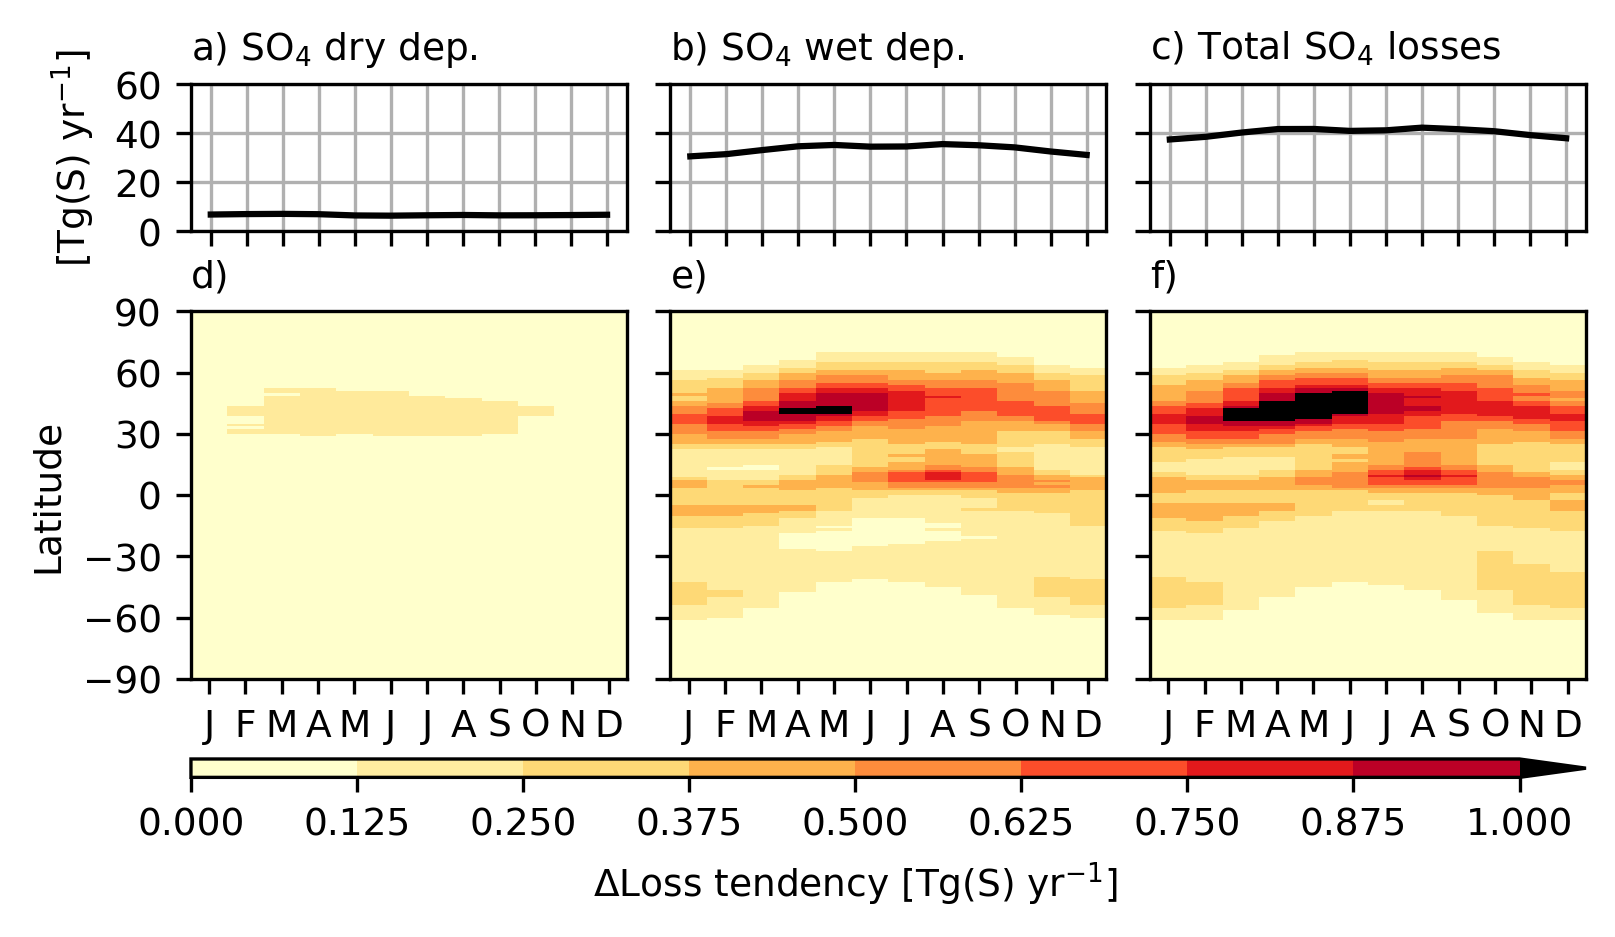
\includegraphics{Chapter4/Figs/so4_losses_histsst_pothole.png}
%     \caption[\ce{SO4} loss tendencies due to oxidation and deposition by months between 1960 and 1989 due to aerosol precursor emissions]{\ce{SO4} loss tendencies due to oxidation and deposition by months 1960 and 1989. (a-c) Total seasonal \ce{SO4} loss tendency. (d-f) \ce{SO4} loss tendency as a function of month of year and latitude. This plot is a difference between \histsst{} and \sstpiaer}
%     \label{fig:ch4:so2-loss}
% \end{figure}



\begin{figure}
    \centering
    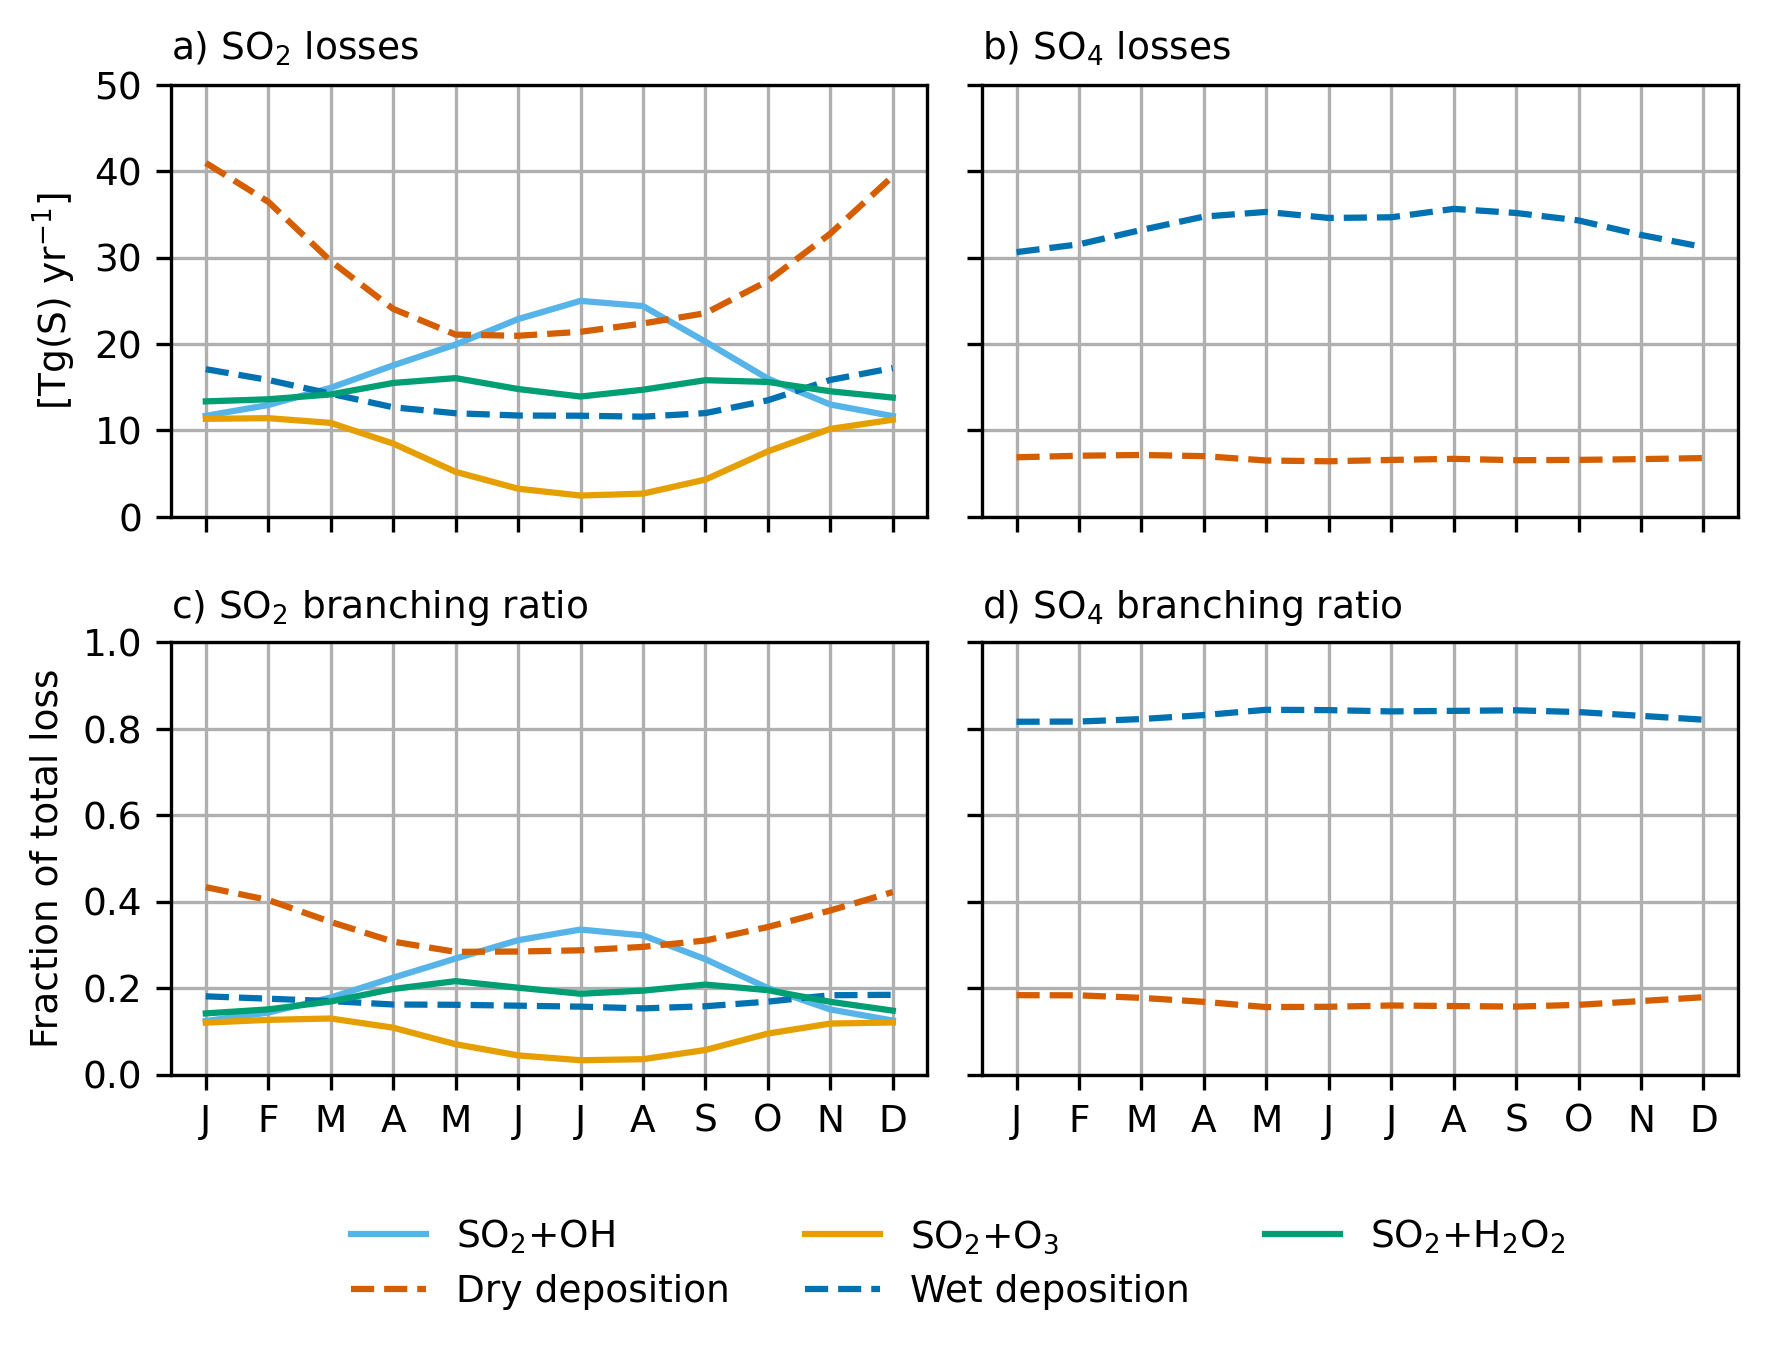
\includegraphics{Chapter4/Figs/branching_ratio_histsst_pothole.png}
    \caption[Absolute and relative losses for \ce{SO2} and \ce{SO4} by month of year between 1960 and 1989]{Absolute and relative losses for \ce{SO2} and \ce{SO4} by month of year between 1960 and 1989. (a-b) Total seasonal \ce{SO2} and \ce{SO4} loss tendency. (c-d) \ce{SO2} and \ce{SO4} loss tendency relative to total losses.}
    \label{fig:ch4:seasonal-branching-ratio}
\end{figure}


Figure \ref{fig:ch4:seasonal-branching-ratio} shows the loss tendencies of \ce{SO2} and \ce{SO4} aggregated by month. It shows that \ce{SO2} may have a different fate depending on the emitted month. During the boreal summer months, 35\% of \ce{SO2} is oxidised by OH, surpassing dry deposition. \ce{SO2 + O3} shows large, but opposite trend to \ce{SO2 +OH}, seasonal variation, contributing less than 10\%  in summer and reaching 15\% in winter. The trend of wet deposition follows emissions, and the fraction of the total loss to which it contributes is largely constant at 18\%. As more \ce{SO2} oxidises and forms \ce{SO4} in summer, \ce{SO4} losses also increase in the same season. However, the ratio between \ce{SO4} wet and dry deposition is relatively constant throughout the year.


\begin{figure}
    \centering
    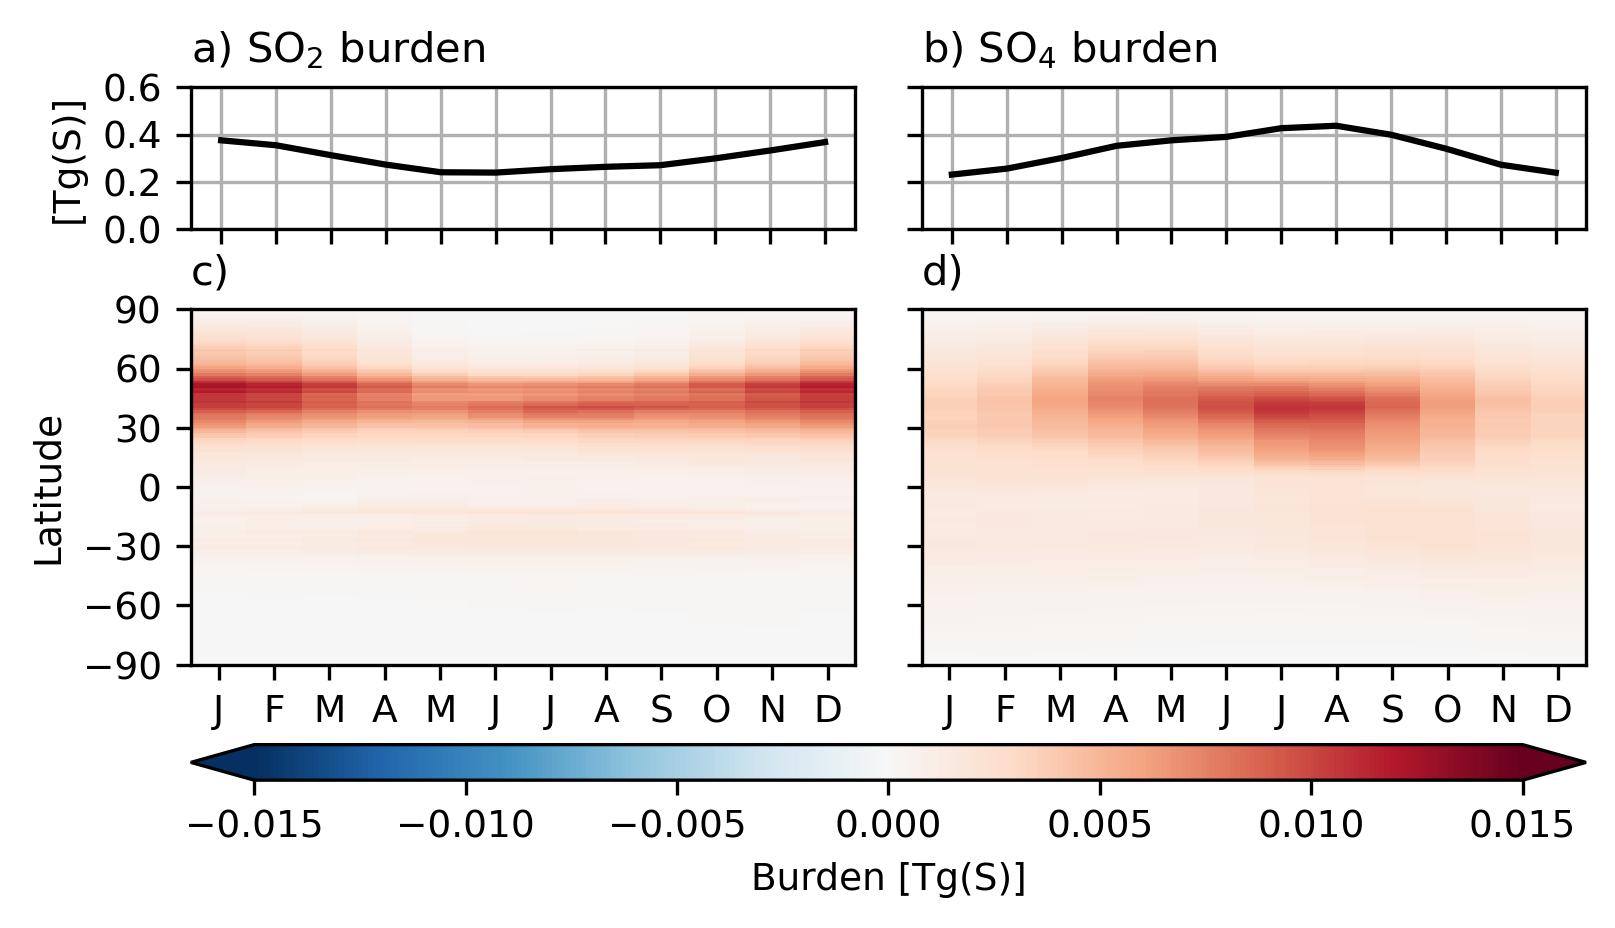
\includegraphics{Chapter4/Figs/seasonal_s_burden_pothole.png}
    \caption[\ce{SO2} and \ce{SO4} mass burden by season between 1960 and 1989]{\ce{SO2} and \ce{SO4} mass burden by season between 1960 and 1989 due to aerosol precursor emissions.}
    \label{fig:ch4:seasonal-s-burden}
\end{figure}

Figure \ref{fig:ch4:seasonal-s-burden} shows the change in \ce{SO2} and \ce{SO4} mass burden due to aerosol precursor emissions. In the northern hemisphere, where emissions are low and oxidation is high in summer, there is a 0.15 Tg(S) decrease in \ce{SO2} burden and subsequent increase in \ce{SO4} burden. The opposite is true when more \ce{SO2} is emitted in boreal winter, resulting in higher \ce{SO2} burden in December and January. 


\begin{figure}
    \centering
    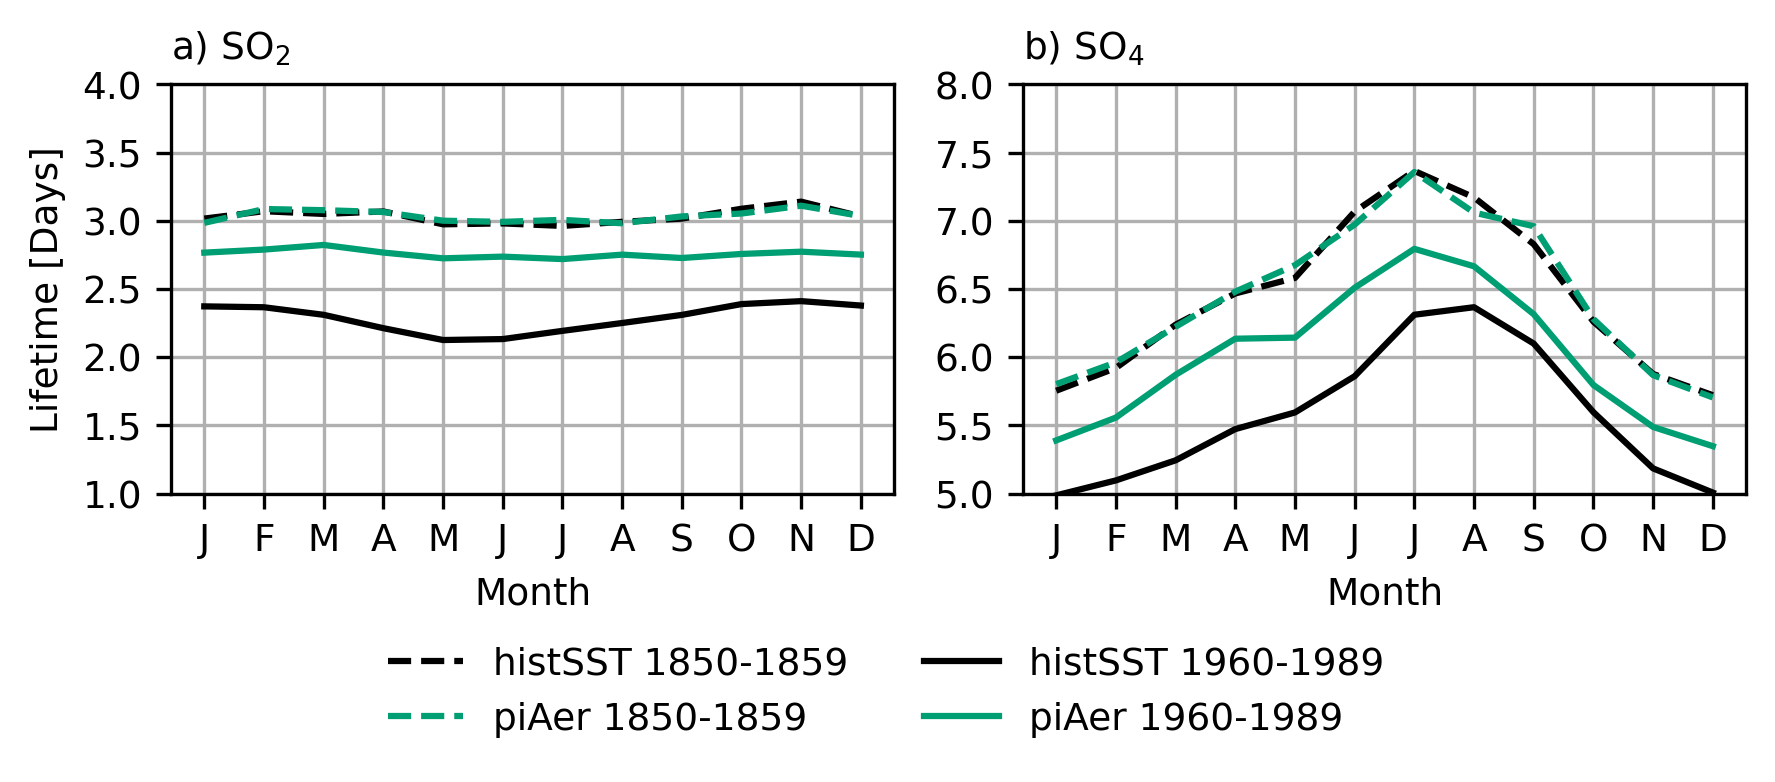
\includegraphics{Chapter4/Figs/lifetime_pothole.png}
    \caption[\ce{SO2} and \ce{SO4} lifetime by season between 1980 and 1989]{\ce{SO2} and \ce{SO4} lifetime by season between 1850--1859 and 1960--1989 from \histsst{} and \sstpiaer{}}
    \label{fig:ch4:seasonal-s-lifetime}
\end{figure}


Variation in loss mechanism modulates \ce{SO2} and \ce{SO4} lifetimes. Figure \ref{fig:ch4:seasonal-s-lifetime} shows a global mean lifetime of \ce{SO2} and \ce{SO4} for two time periods, 1850--1859 and 1960--1989, aggregated by month. When \ce{SO2} emissions are at the 1850 level, \ce{SO2} lifetimes show a slight variation across seasons, as seen in both \sstpiaer{} trends (solid and dashed green lines) and \histsst{} (dashed black line) in the 1850s. Whether this slight variation is due to an additional 0.75 \unit{Tg(S)~yr^{-1}} of emission in winter (Figure \ref{fig:app1:seasonal-emiso2-1850}) or from the variation in loss processes is inconclusive. 

The higher oxidants in the atmosphere decrease the \ce{SO2} lifetime by increasing oxidation, as seen in Chapter \ref{ch3:title}. The average \ce{SO2} lifetime decreases from 3 days to 2.75 days when oxidant level increases in the 1980s even when \ce{SO2} emissions are constrained at the 1850s level as shown by the \sstpiaer{} simulation (dashed green line versus solid green line). \ce{SO2} emissions in the 1980s decreased its mean lifetime further by 0.75 days and exacerbated the seasonal variation compared to the 1850s. The lowest \ce{SO2} lifetime is observed in May and June of the pothole period, approaching 2.0 days from the original 3.0 days in the 1850s. It could be said that \ce{SO2} emission increase at the surface drives the lifetime down. 

\ce{SO4} aerosol lifetime shows a greater variation across the season, even in the 1850s, with a shorter lifetime in winter at 5.7 days and a longer lifetime in summer at 7.3 days, showing a difference of 1.5 days between seasons. \ce{SO4} production mainly comes from \ce{SO2} oxidation which is higher during summer months (at 30 \unit{Tg(S)~yr^{-1}} compared to 20 \unit{Tg(S)~yr^{-1}} in winter; Figure \ref{fig:ch4:so2-loss}). While \ce{SO4} wet deposition increases in summer, the rate of increase is lower than production (an increase of 5 \unit{Tg(S)~yr^{-1}} between winter and summer), resulting in a higher burden and longer lifetime. 


Regarding the model performance against observations, the simulated surface \ce{SO2} and \ce{SO4} concentrations were evaluated against ground-based measurement networks in the USA and Europe by \citet{hardacreEvaluationSO2SO422021}. In polluted areas, UKESM1 overpredicts surface \ce{SO2} by a factor of 3 while underpredicts surface \ce{SO4} by 25--35\%. The mean surface \ce{SO2} concentration is overestimated, especially in summer for the 33 Eastern American ground observation sites for the period 1987--2014 \citep{hardacreEvaluationSO2SO422021}. This hints towards a better removal process for the model. 


The updated UKESM1 with modified \ce{SO2} dry deposition scheme, called UKESM1.1, has a lower surface \ce{SO2} concentration, but this exacerbates the underprediction of \ce{SO4} \citep{mulcahyUKESM1DevelopmentEvaluation2022}. This points towards the possibility that the model may need further compensation for the sulfur cycle and an increase in chemical oxidation of \ce{SO2} to convert \ce{SO2} in \ce{SO4} and potentially too large dry deposition \citep{mulcahyUKESM1DevelopmentEvaluation2022}.

% Comment on the seasonal cycle of sulfate
Overall, this section shows that seasonal changes in oxidants, cloud fractions and depositions significantly affect the fate of \ce{SO2}. \ce{SO2} emitted in summer has a greater chance of being oxidised, especially by OH, forming new \ce{SO4} aerosol particles and affecting the climate. On the other hand, \ce{SO2} emitted in winter persists in the atmosphere as a more significant burden for a longer time and can potentially be air pollutants affecting the local population and the environment. 


\subsection{Seasonal cycle of aerosol properties due to aerosol precursors}

\ce{SO2} oxidation and \ce{SO4} aerosol formation are coupled in UKESM1. Aerosol mass and number are independently diagnosed, allowing us to examine the variation in aerosol properties and size distribution due to oxidation changes. We observed more gas-phase oxidation in the boreal summer in the previous section. This section examines the aerosol properties that result from oxidation in different seasons.


\begin{figure}
    \centering
    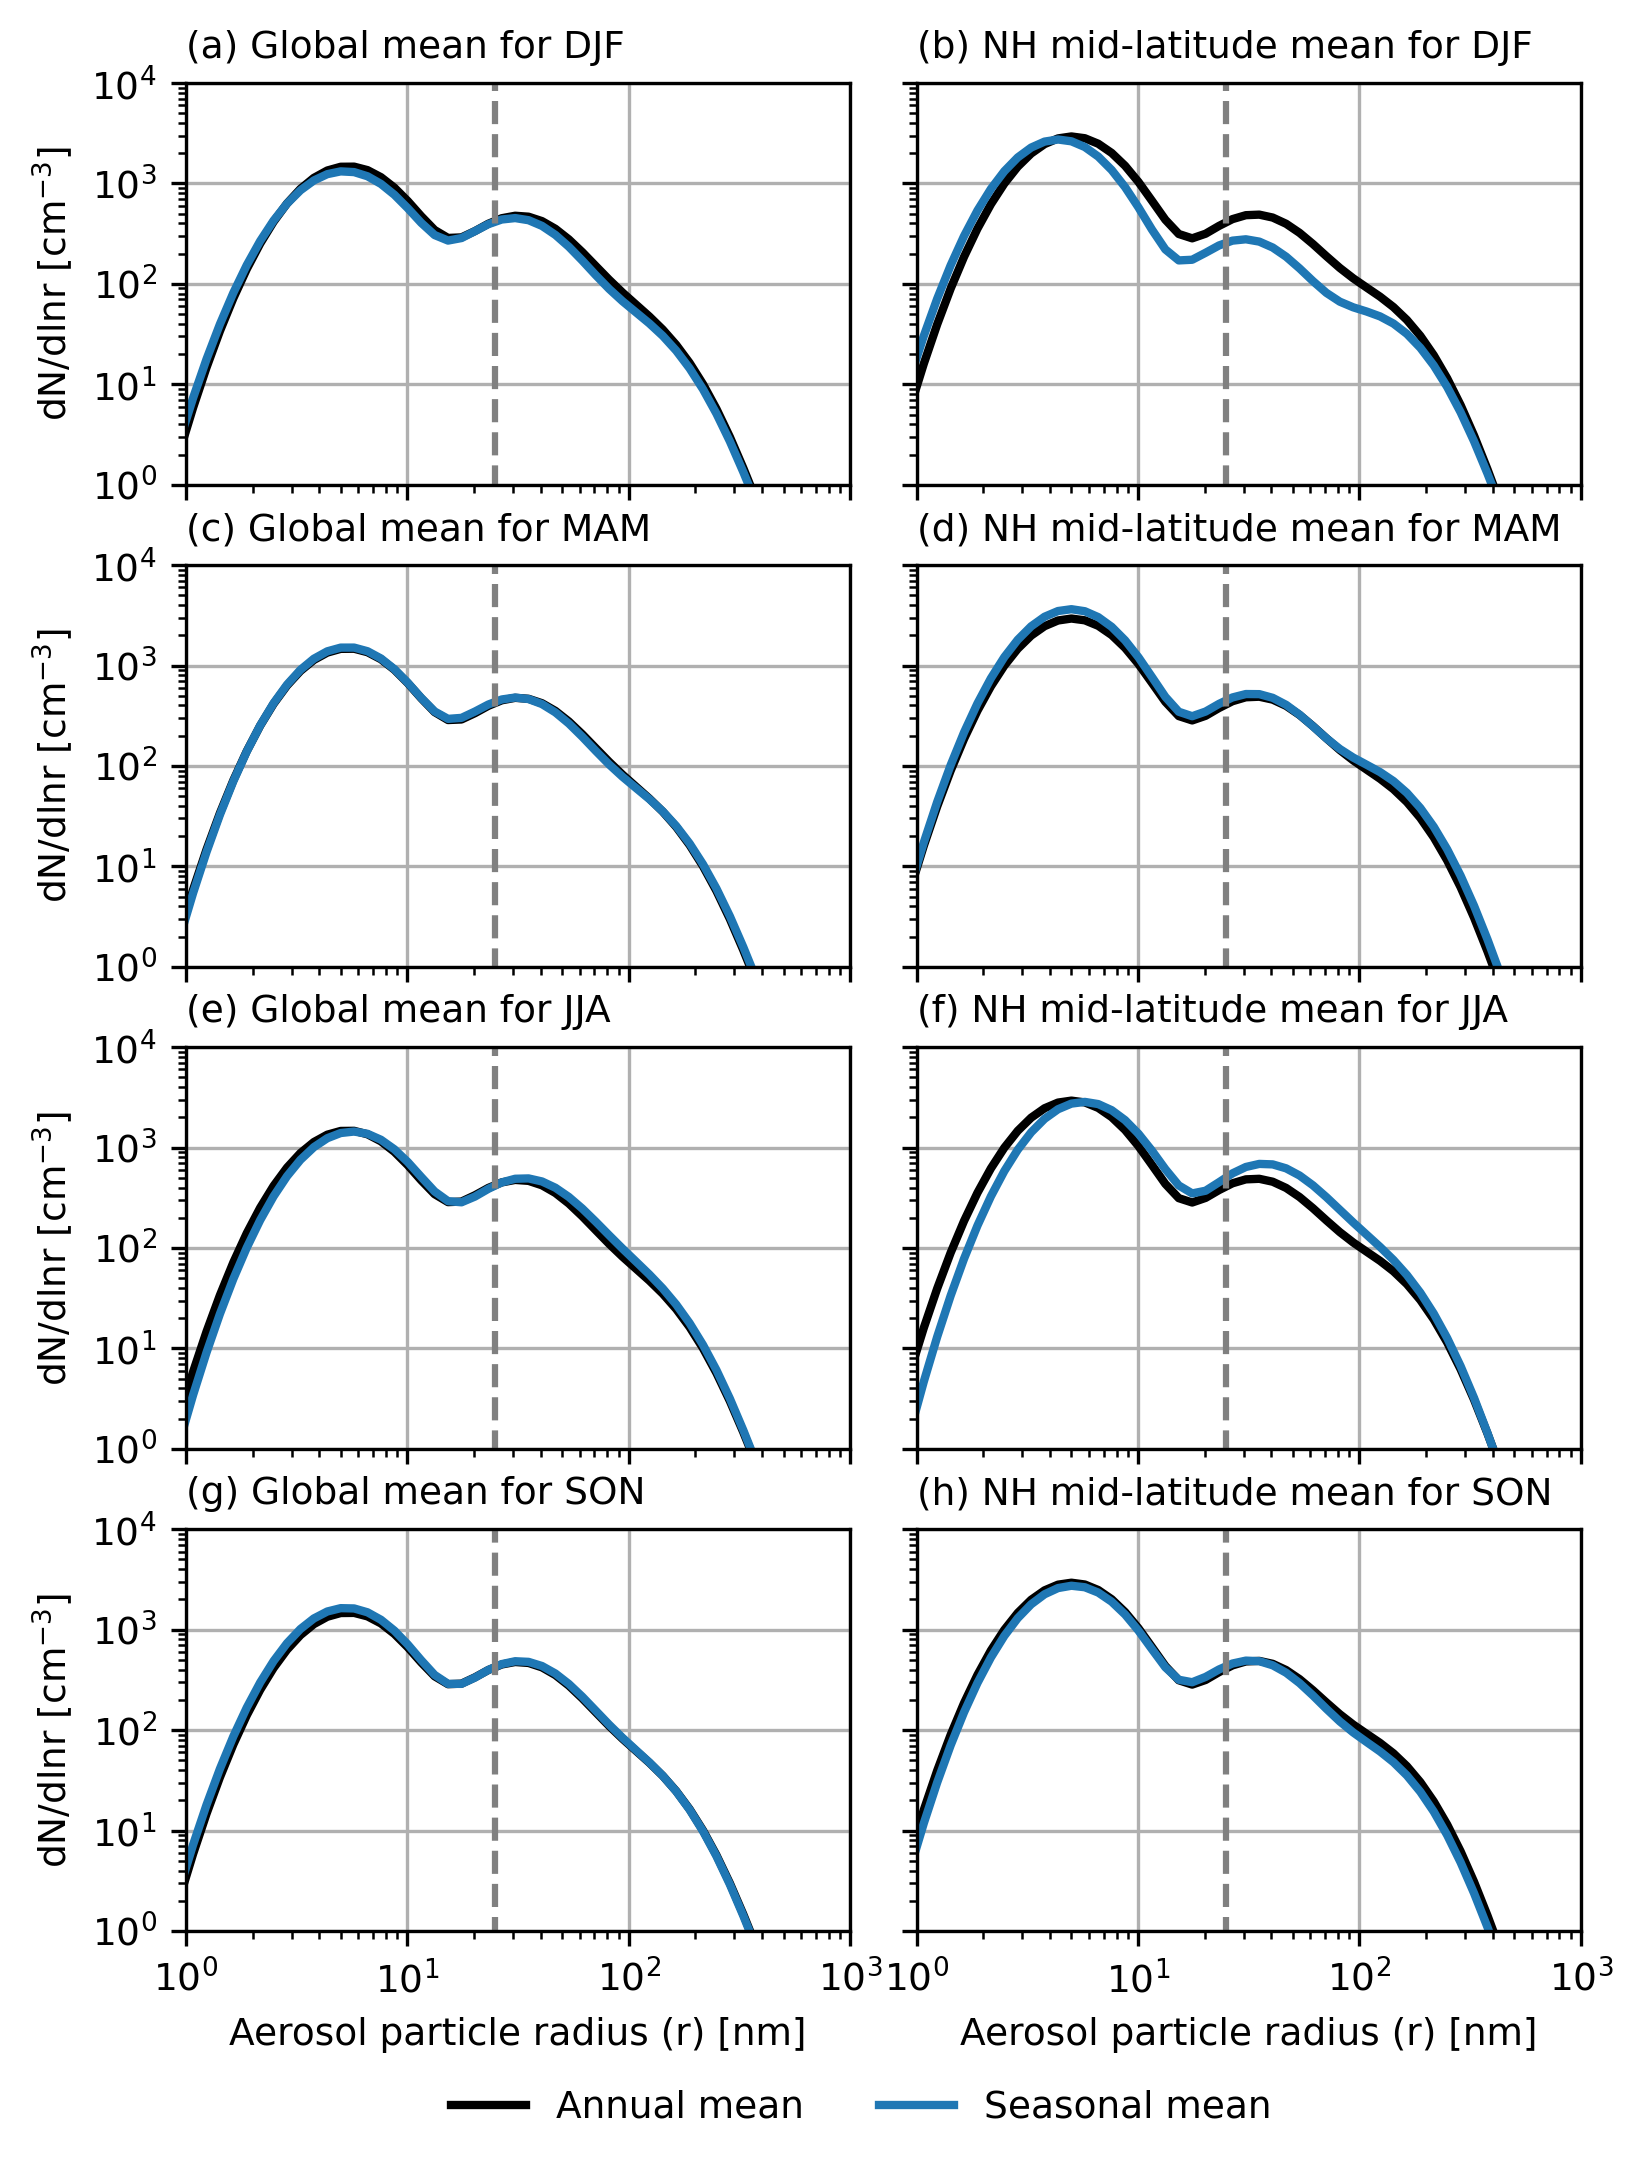
\includegraphics{Chapter4/Figs/seasonal_aerosol_size_dist_1980.png}
    \caption[Mean aerosol size distribution from the surface up to 10 km between 1980 and 1989 aggregated by seasons]{Mean aerosol size distribution from the surface up to 10 km between 1980 and 1989 aggregated by seasons. The black solid lines denote the domain annual mean. The blue lines denote the respective seasonal mean for each panel. The first column (sub-figure a, c, e, and g) shows the global mean aerosol size distribution. The second column (sub-figure b, d, f, and h) shows the mean between 30--60\textdegree N. The dashed vertical line indicates an aerosol radius of 25 nm, defined as N50 or aerosol with a diameter above 50 nm.}
    \label{fig:ch4:seasonal-aerosol-size}
\end{figure}


Figure \ref{fig:ch4:seasonal-aerosol-size} shows the variation in aerosol size distribution across the four seasons and a reference annual mean in black lines. The plots cover all aerosol components with aerosol size distribution up to accumulation mode aerosol ($\bar{r} = 1000$ \unit{\nano\metre} or $\bar{D} < 2000$ \unit{\nano\metre}) as coarse mode aerosol number concentration is negligible due to its low concentration. In the boreal summer months, June, July and August (JJA), the global mean aerosol size distribution shows minor changes to global mean aerosol size distribution (left columns) in all seasons. However, the changes are more observable in the northern hemisphere mid-latitude (30\textdegree--60\textdegree N; right column). The aerosol size distribution in winter (December, January and February; DJF) is lower than the annual mean, especially for aerosol with a radius greater than 25 \unit{\nano\metre} or diameter above 50 \unit{\nano\metre} (N50), which acts as cloud condensation nuclei. The opposite is true for the same region over summer (June, July and August; JJA) when we have observed more gas-phase oxidation.


The \ce{SO2} oxidation pathways could explain the shift in aerosol size distribution in summer and winter and how the model simulates aerosol processes. In UKESM1, \ce{SO2} gas-phase reaction produces \ce{H2SO4} gas, which condenses into new nucleation mode aerosol particles \citep{mannDescriptionEvaluationGLOMAPmode2010}. On the other hand, \ce{SO2} aqueous-phase reactions add \ce{SO4} mass onto the existing aerosols in accumulation and coarse mode without forming new particles. As we saw from the previous section, there is more \ce{SO2 + OH} reaction during summer. This additional aerosol particle production increases the accumulation mode (peaks at a 30 nm radius) aerosol number in summer. 


\begin{figure}
    \centering
    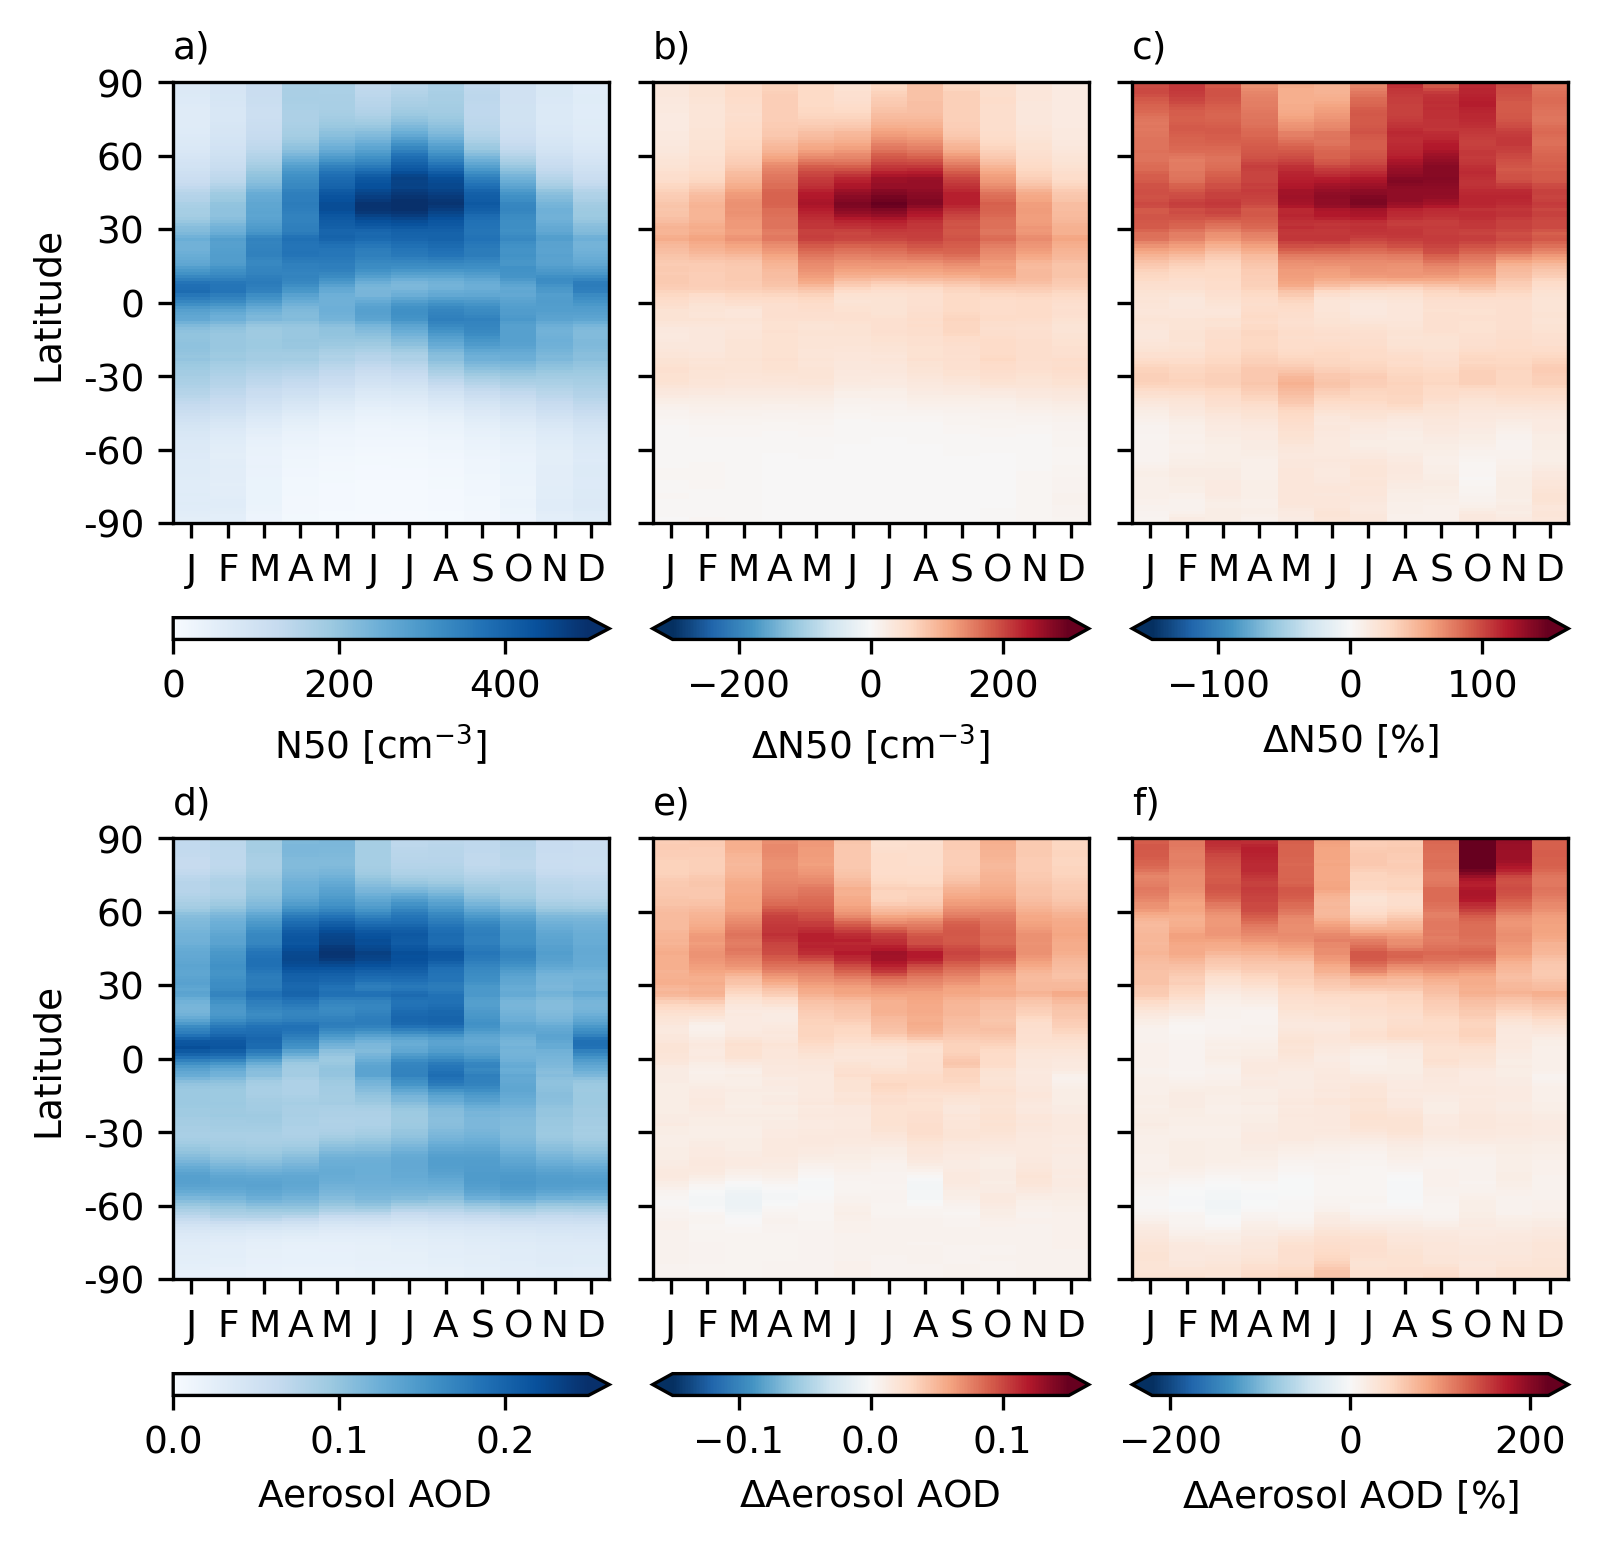
\includegraphics{Chapter4/Figs/seasonal_aerosol_props_1980.png}
    \caption[Mean AOD at 550 nm and N50 between 1980 and 1989 as a function of months and latitude due to aerosol precursor emissions]{mean (a--c) number concentration of aerosol with a diameter greater than 50 nm (N50) from the surface up to 10 km and (d--f) AOD at 550 nm between 1980 and 1980 as a function of months and latitude. The first column is the absolute value, and the second and third columns are the changes in aerosol properties due to aerosol precursor emissions (\histsst{} minus \sstpiaer{}) in absolute and relative terms, respectively.}
    \label{fig:ch4:seasonal-aerosol-props}
\end{figure}


Aerosol properties such as AOD and aerosol number concentration, especially for N50, are quantities that link to radiative adjustment due to aerosols. Figure \ref{fig:ch4:seasonal-aerosol-props} shows aerosol macroscopic properties, including the AOD and N50 concentration and the changes due to aerosol precursor emissions. Aerosol precursor emission adds more than 200 \unit{cm^{-3}} or more than 150\% to N50 between June and August in the Northern Hemisphere. Although there are more significant \ce{SO2} emissions in the same region in winter, this translates into lesser growth in N50 of approximately 50\%.


Aerosol optical depth (AOD) quantifies the absorption or scattering of light by the aerosol layer in the atmosphere, providing a measure of aerosols' columnar concentration in the atmosphere. Aerosol AOD shows a slightly different seasonal trend from N50. While there is an increase in AOD in summer when more oxidation is observed, the seasonal trend agrees better with the \ce{SO4} burden in Figure \ref{fig:ch4:seasonal-s-burden}. 


Studies show that UKESM1 and GLOMAP-mode, its aerosol component, are skilful in predicting sulfate aerosol trends between 1980 and 2009, with the tendency to underpredict sulfate aerosol concentration in Europe and East Asia compared to observations \citep{mannDescriptionEvaluationGLOMAPmode2010, mulcahyDescriptionEvaluationAerosol2020}.  The model well predicts the spatial distribution of sulfate aerosol distribution but consistently underpredicts the absolute values for all years, although it is within the observed variability. The model also underpredicts East Asian observations to a greater degree than GC3.1, a model with the same physical atmosphere-ocean and aerosol component but a lower level of interaction within the Earth system. With the updated dry deposition scheme in UKESM1.1, the model further underpredicts sulfate aerosol loading \citep{hardacreEvaluationSO2SO422021}. As discussed in the next section, even with underpredicted sulfate aerosol, the model shows a substantial change in cloud properties compared to other Earth system models. 


\subsection{Seasonal cycle of cloud properties}

Aerosol acts as cloud condensation nuclei, allowing water vapour to condense at lower temperatures than homogeneous nucleation. Thus, the change in aerosol number and size modifies cloud properties \citep[e.g. ][]{rosenfeldGlobalObservationsAerosolcloudprecipitationclimate2014, boucherCloudsAerosols2014,persadAerosolsMustBe2022}. Aerosol in the cloud increases its albedo and lifetime, leading to weather and climate effects \citep{twomeyInfluencePollutionShortwave1977, albrechtAerosolsCloudMicrophysics1989}. This section aims to quantify the change in cloud properties due to aerosol precursor emissions in different seasons.

\begin{figure}
    \centering
    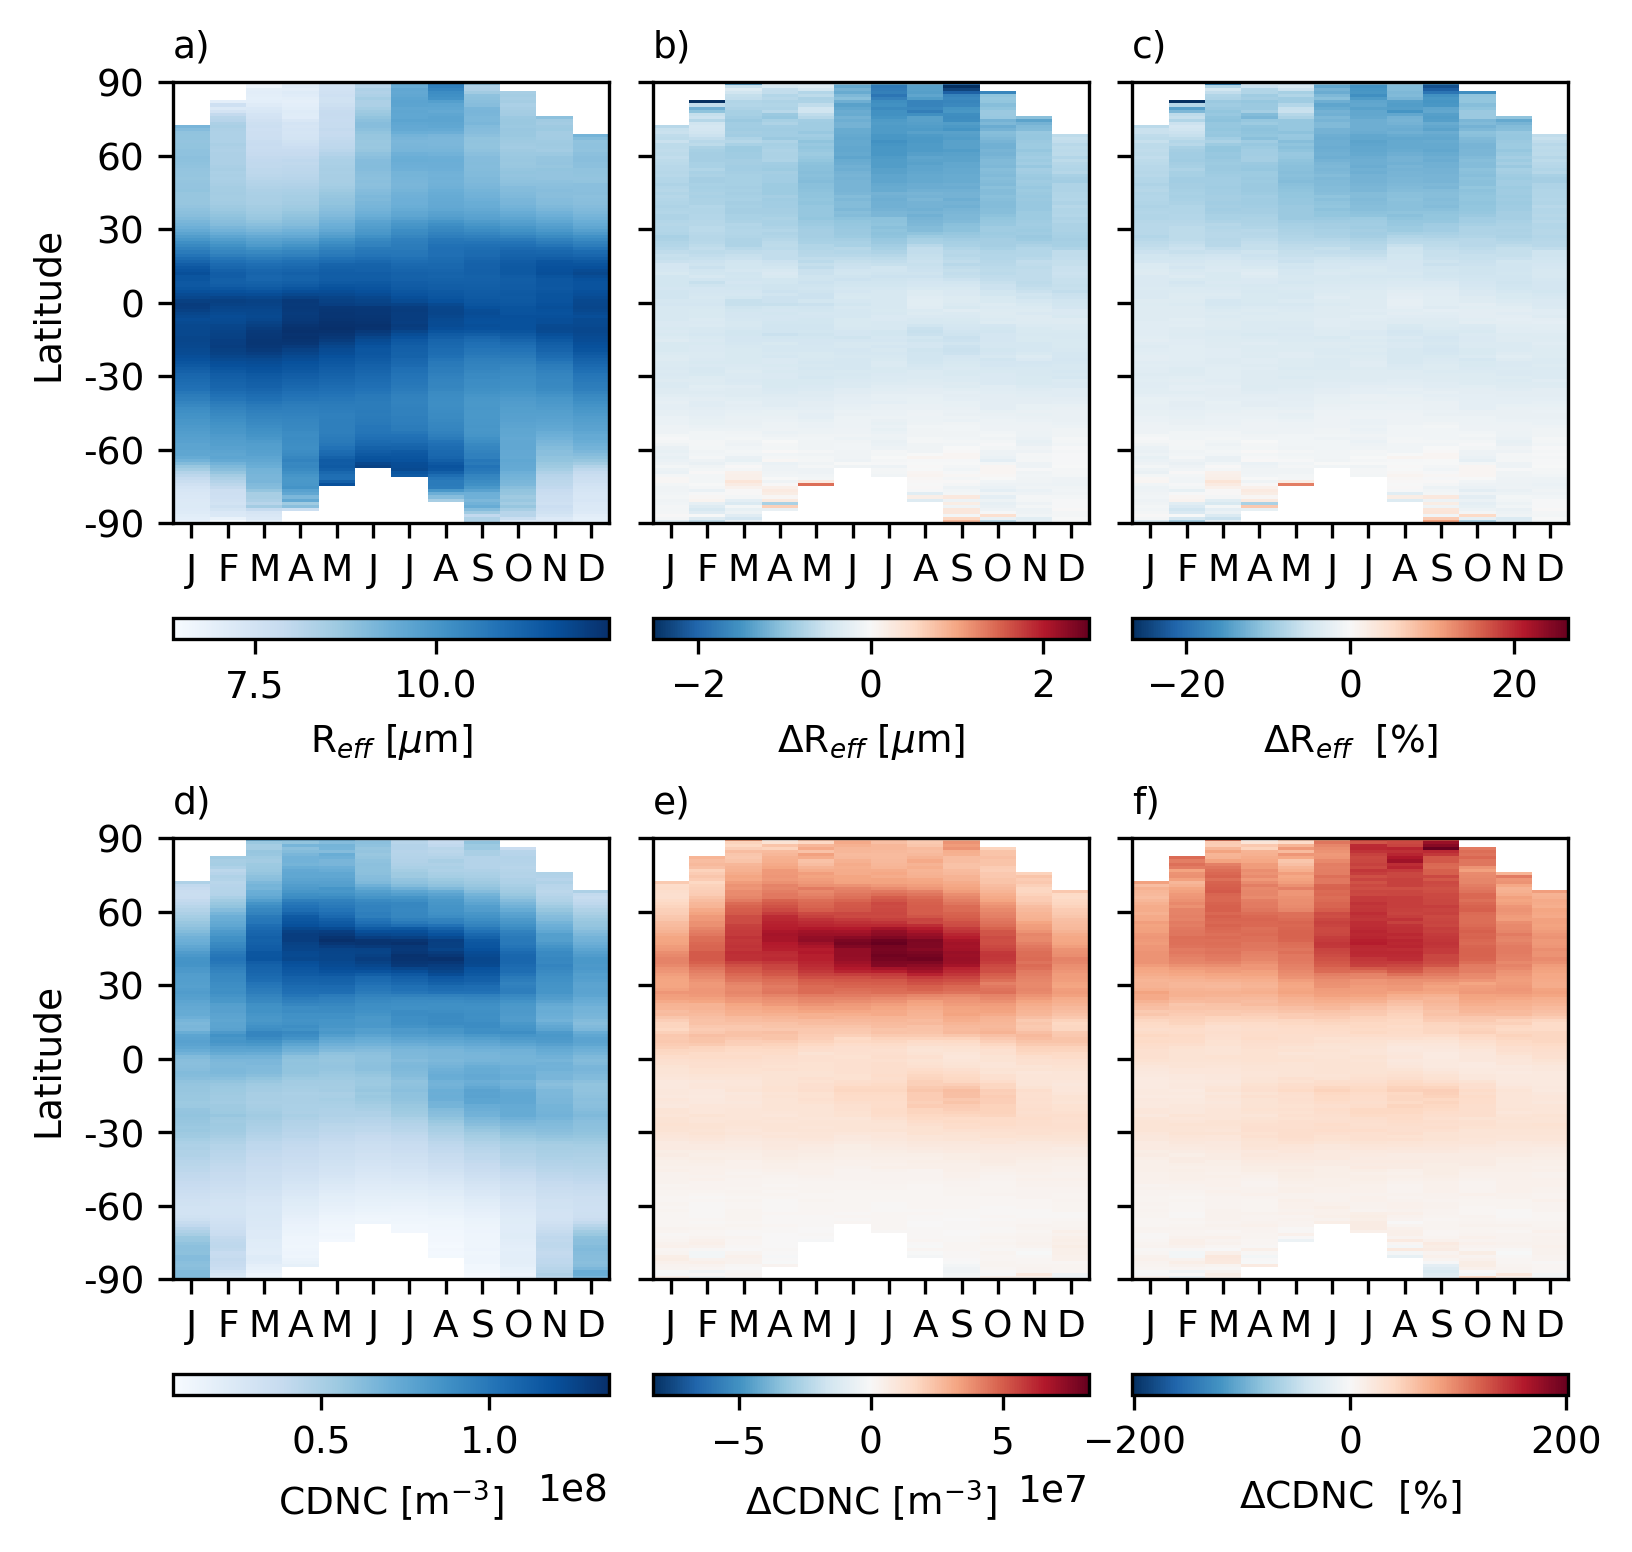
\includegraphics{Chapter4/Figs/seasonal_cloud_props1_pothole.png}
    \caption[\Reff{} and CDNC aggregated by latitude and month between 1960 and 1989]{a) shows mean \Reff{} from \histsst{} aggregated by latitude and month between 1960 and 1990 below 10 km. b-c) shows the change in \Reff{} due to aerosol precursor emissions (\histsst{} minus \sstpiaer{}) in absolute value and the percentage of change compared to \sstpiaer{}, respectively. d-f) show a similar analysis for CDNC.}
    \label{fig:ch4:seasonal-cloud-props1}
\end{figure}


Figure \ref{fig:ch4:seasonal-cloud-props1} shows the effect of aerosol precursor emissions on cloud properties. Cloud droplet effective radius, \Reff{}, at 30 to 60 \textdegree N is decreased by approximately \qty{1.5}{\micro\metre} or 10\% between June and September. The cloud droplet number concentration, CDNC, sees a more significant change at 100\% at the same month and latitude. 



\begin{figure}
    \centering
    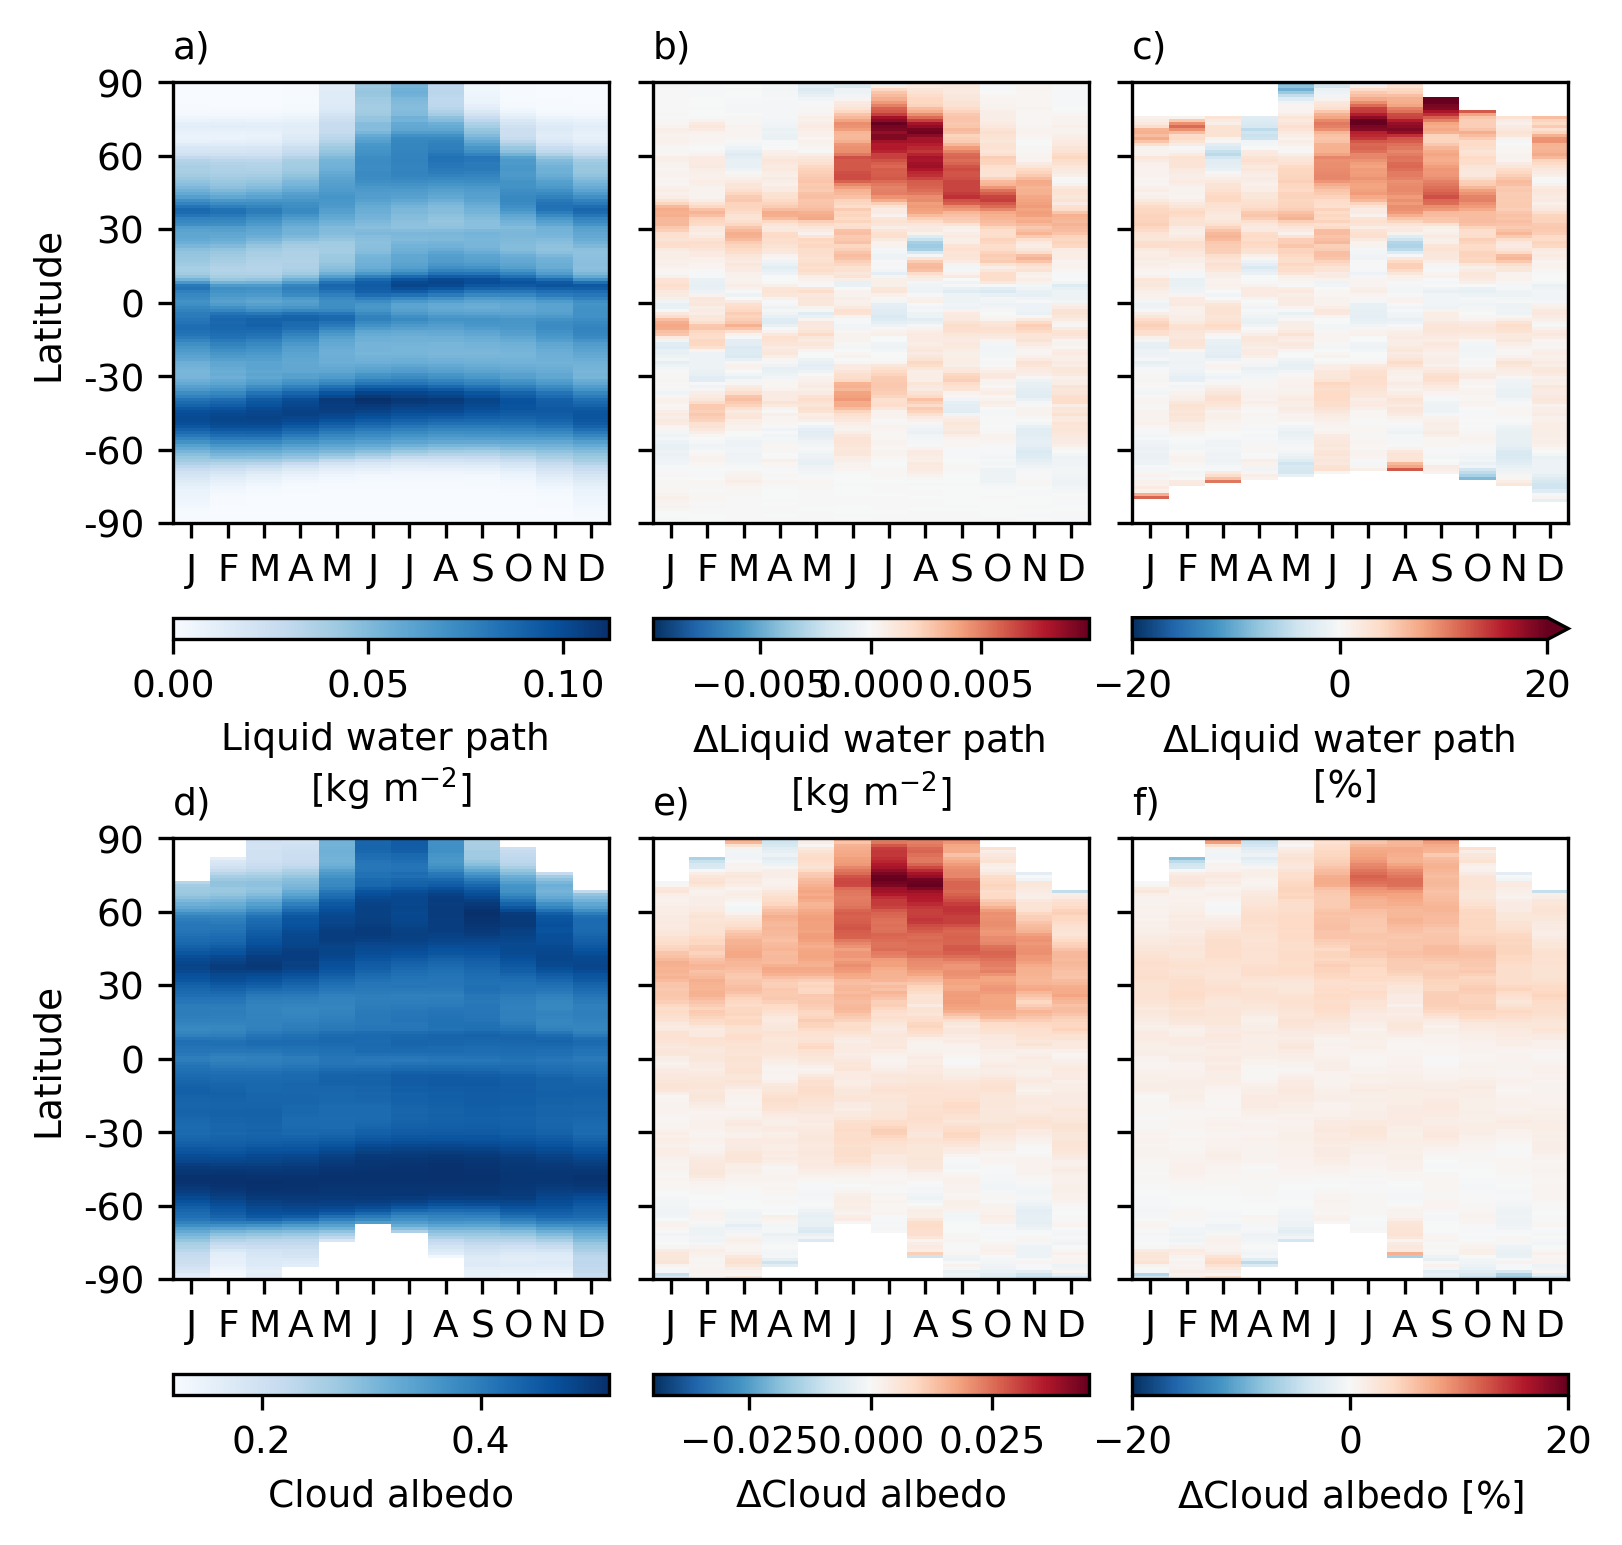
\includegraphics{Chapter4/Figs/seasonal_cloud_props2_pothole.png}
    \caption[Cloud liquid water path and albedo aggregated by latitude and month between 1960 and 1989]{a) shows mean liquid water path from \histsst{} aggregated by latitude and month between 1960 and 1990 below 10 km. b-c) shows the change in liquid water path due to aerosol precursor emissions (\histsst{} minus \sstpiaer{}) in absolute value and the percentage of change compared to \sstpiaer{}, respectively. d-f) show a similar analysis for cloud albedo.}
    \label{fig:ch4:seasonal-cloud-props2}
\end{figure}

Cloud reflectance increases as the droplet size decreases. Figure \ref{fig:ch4:seasonal-cloud-props2} shows the cloud liquid water path, the vertical integration of cloud liquid water content and cloud albedo. The liquid water path in the northern hemisphere, especially during summer, increases by 15--20\% due to aerosol precursor emissions. This results in a 10\% more reflective cloud in boreal summer. The result shows that the effect of aerosol precursors on cloud is localised and correlates to \ce{SO2} oxidation rather than emissions.

% Discuss cloud simulation in UKESM1 and any validations of this run
While the results above show substantial cloud response to aerosol precursors, most cloud properties exhibit a low bias compared to MODIS satellite measurements from March 2009 to March 2010 in the North Atlantic Ocean region \citep{grosvenorDecompositionCloudAerosol2020}. According to \citet{grosvenorDecompositionCloudAerosol2020}, the atmosphere-only version of UKESM1 can capture the cloud spatial pattern with a spatial correlation above 0.8 but consistently underestimates cloud cover and liquid water path. Low- and mid-altitude cloud fraction is lower by a normalised mean bias factor (NMBF) of -28--37\%. The high altitude cloud is the least biased at -8.5\%. In-cloud liquid water path is also underestimated with NMBF of -20\%. In contrast, cloud droplet number concentration is overestimated by 11.3\%.

\change[inline]{Add discussion on the impact of GLOMAP-mode on aerosol forcing in HadGEM3 https://acp.copernicus.org/articles/13/3027/2013/}

It is essential to note that UKESM1 has the largest change in cloud fraction from aerosol precursor emissions amongst 6 ESMs with interactive chemistry and aerosol schemes that participated in AerChemMIP \citep{zhangRoleAnthropogenicAerosols2021}. While UKESM1 underestimates cloud fraction, it also has the strongest sensitivity to aerosol loading \citep{zhangRoleAnthropogenicAerosols2021}, but model aerosol sensitivity does not predict pothole cooling. More comparison is needed between models to diagnose the underpinning aerosol and process that leads to pothole cooling. 


\subsection{Seasonal cycle of ERF due to aerosol precursors}


I have shown that \ce{SO2} emissions increase during boreal winter with more energy demands, but aerosol formation does not follow seasonal emission trends. Instead, new \ce{SO4} aerosol particles form when more OH is present for gas-phase oxidation, leading to more aerosol number concentration and brighter clouds in boreal summer. This section discusses the seasonal trend in aerosol-radiation interaction and establishes the correlation between ERF and oxidation processes. Finally, I show quantitatively that the emission timing is responsible for more aerosol formation in summer using the concept of specific ERF.


\begin{figure}
    \centering
    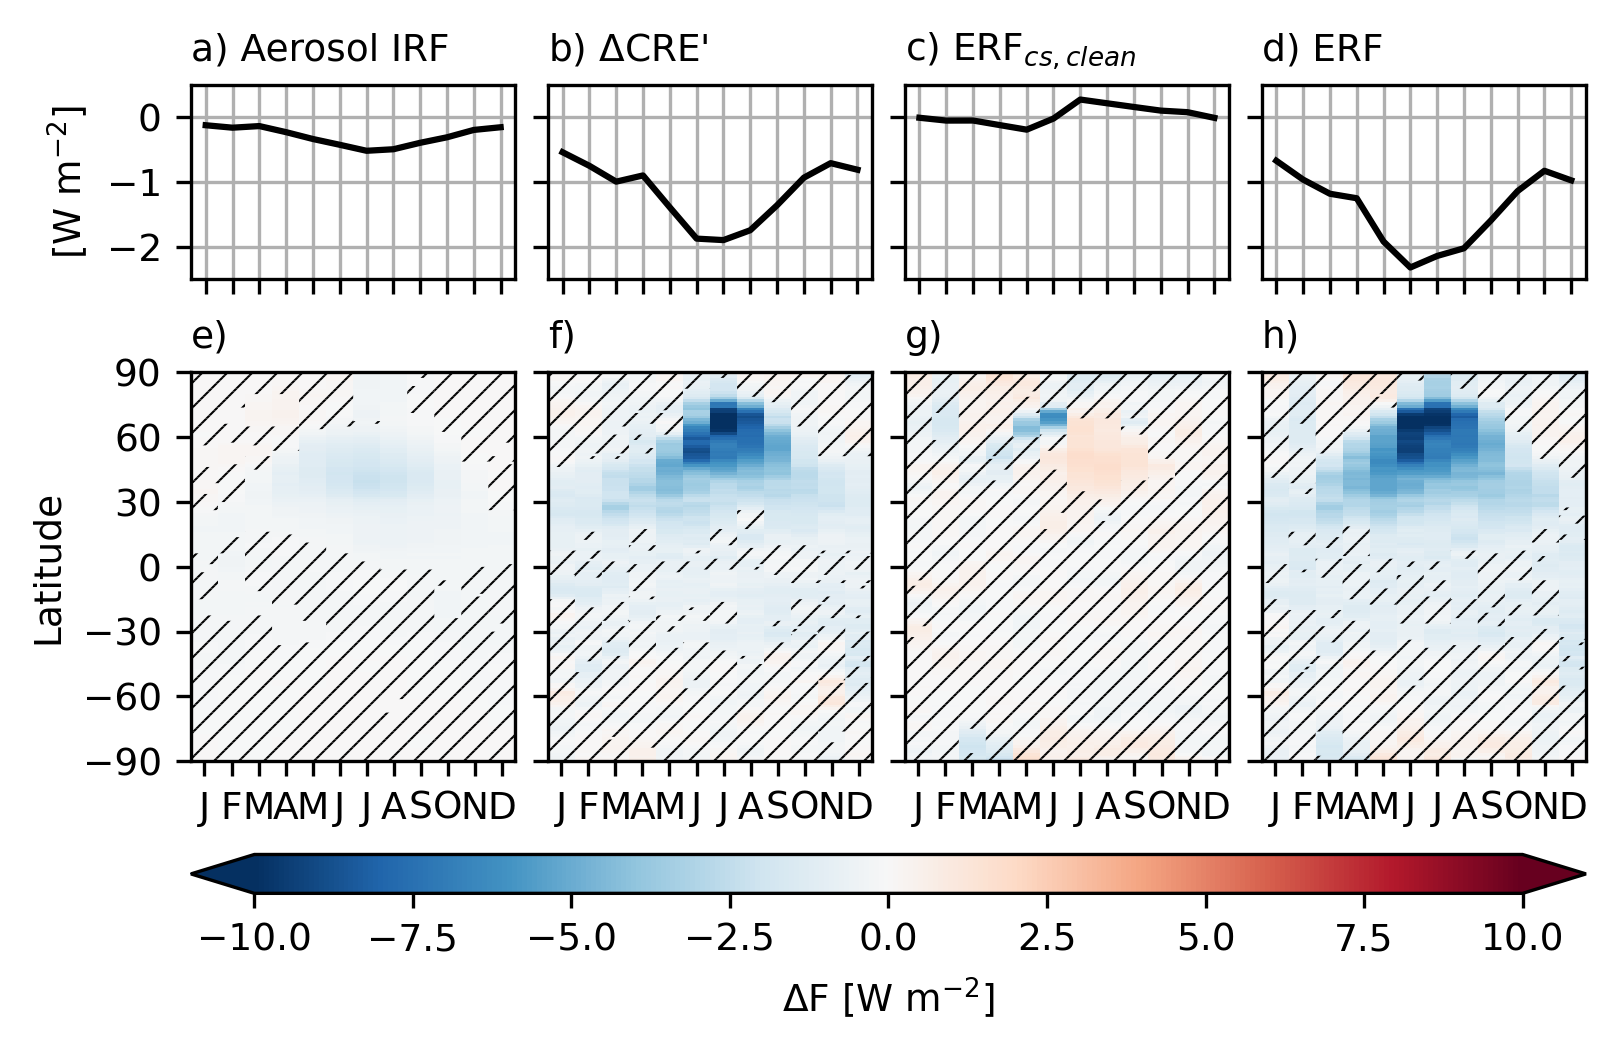
\includegraphics{Chapter4/Figs/latitudinal_erf_sstpiaer-histsst_pothole.png}
    \caption[ERF due to aerosol precursor emissions between 1960--1989 aggregated by month and latitude]{ERF due to aerosol precursor emissions between 1960--1989 aggregated by month and latitude. Each data point is averaged longitudinally, giving 10 data points for each month and latitude. Hatch denotes points where the difference between \histsst{} and \sstpiaer{} is insignificant (p$\leq$0.05).}
    \label{fig:ch4:seasonal-erf}
\end{figure}


Contrary to the assumed correlation between emissions and ERF. Figure \ref{fig:ch4:seasonal-erf} shows a strong seasonal cycle with a high negative in the boreal summer between 1960 and 1989, when \ce{SO2} emissions are lowest annually. Aerosols have less radiative impacts in boreal winter above latitude 45\textdegree N even though \ce{SO2} emission is the strongest in winter. 


% Discuss the ERF from different cloud adjustments
Aerosol radiative effects act mainly in the shortwave. The atmosphere-only version of UKESM1 shows a negative bias in low-altitude cloud fraction with -28.1\% NMBF while overestimating shortwave outgoing radiation at the top of the atmosphere by 1.7--5.8\% NMBF compared to the MODIS satellite observation in the present-day simulation \citep{grosvenorDecompositionCloudAerosol2020}. CDNC is underestimated in the northern North Atlantic Ocean region but overestimated in the southern North Atlantic Ocean by 21.5\%. However, this does not contribute substantially to the bias of outgoing shortwave radiation at the top of the atmosphere \citep{grosvenorDecompositionCloudAerosol2020}. This shows that the model predicts a radiation response from clouds over the Northern Atlantic that is too strong. Whether this correlation applies to other regions is unknown.


\begin{figure}
    \centering
    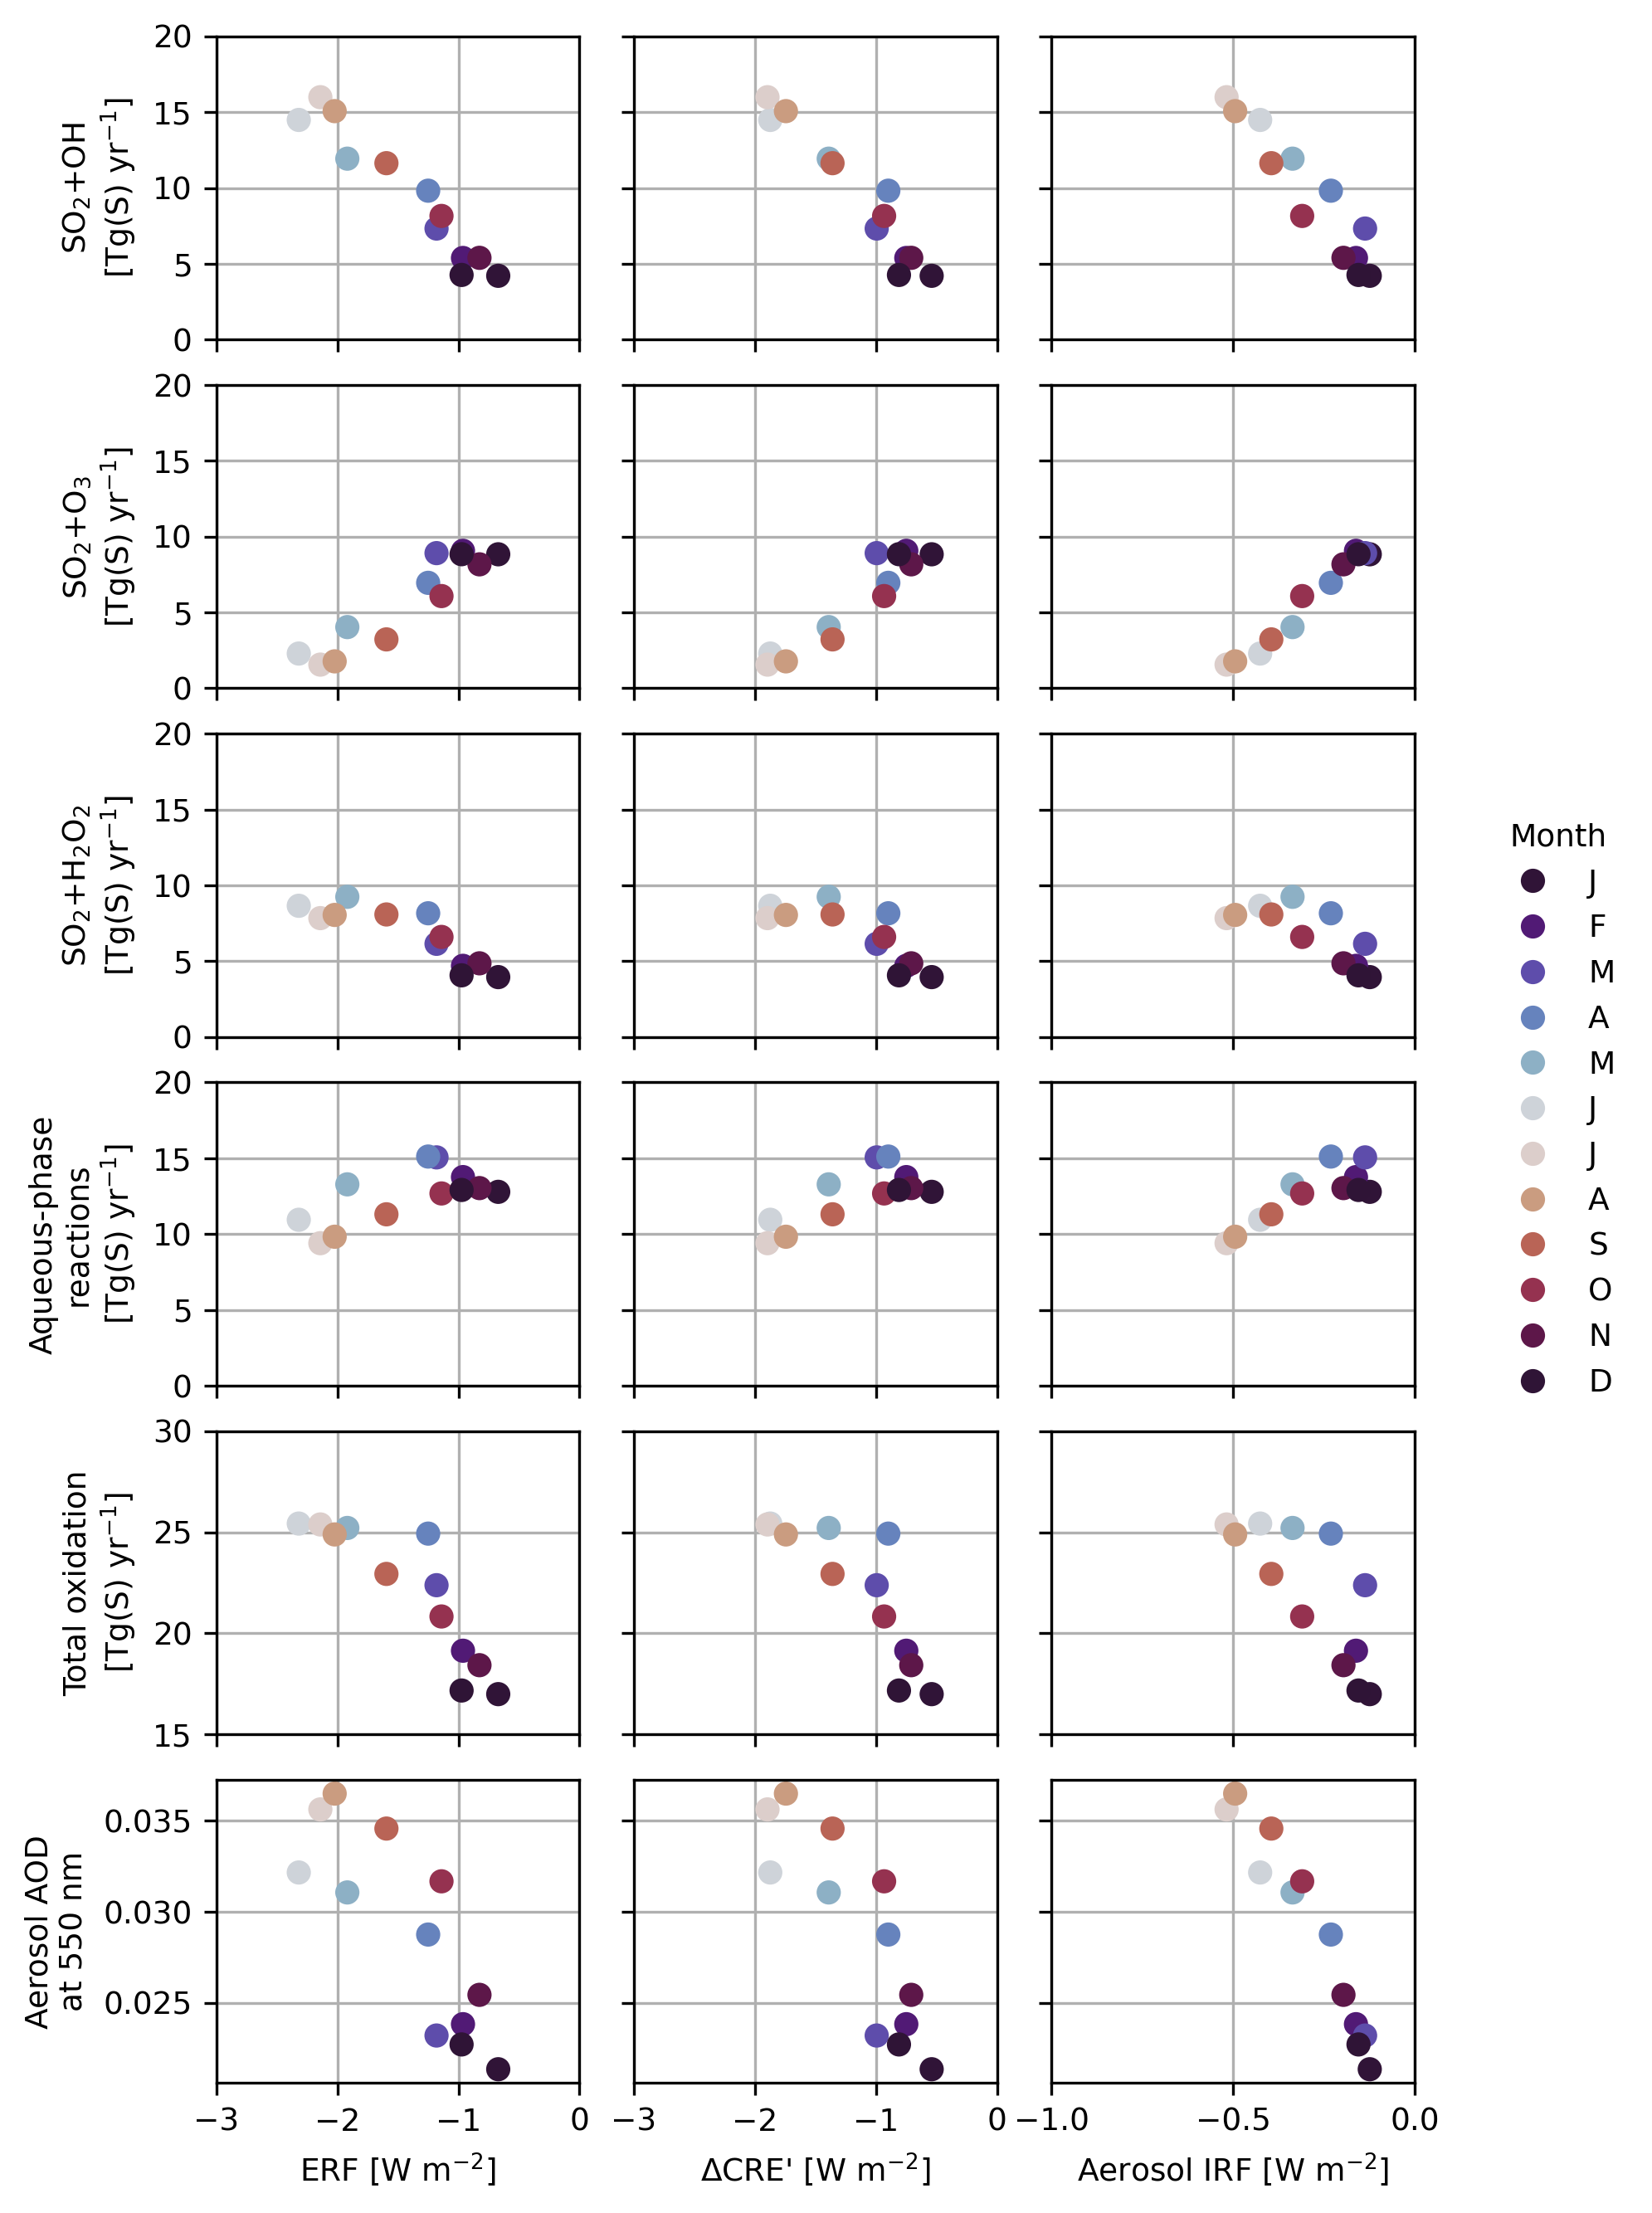
\includegraphics[width=\linewidth]{Chapter4/Figs/seasonal_oxidation_erf_corr_pothole.png}
    \caption[Correlation between \ce{SO2} oxidation tendencies and ERF between 1960 and 1989]{Correlation between \ce{SO2} oxidation tendencies and ERF between 1960 and 1989}
    \label{fig:ch4:seasonal-erf-corr}
\end{figure}

Figure \ref{fig:ch4:seasonal-erf-corr} shows the correlation between oxidation, AOD and radiative forcing. \ce{SO2 + OH} shows an inverse linear relationship with ERF, with greater oxidation tendency and more negative ERF in June--August. Neither total oxidation nor aerosol AOD correlate well with ERF. This suggests that gas-phase oxidation is a valuable parameter for this type of analysis. This plot indicates that oxidation tendencies explain ERF and not emission.


\begin{figure}
    \centering
    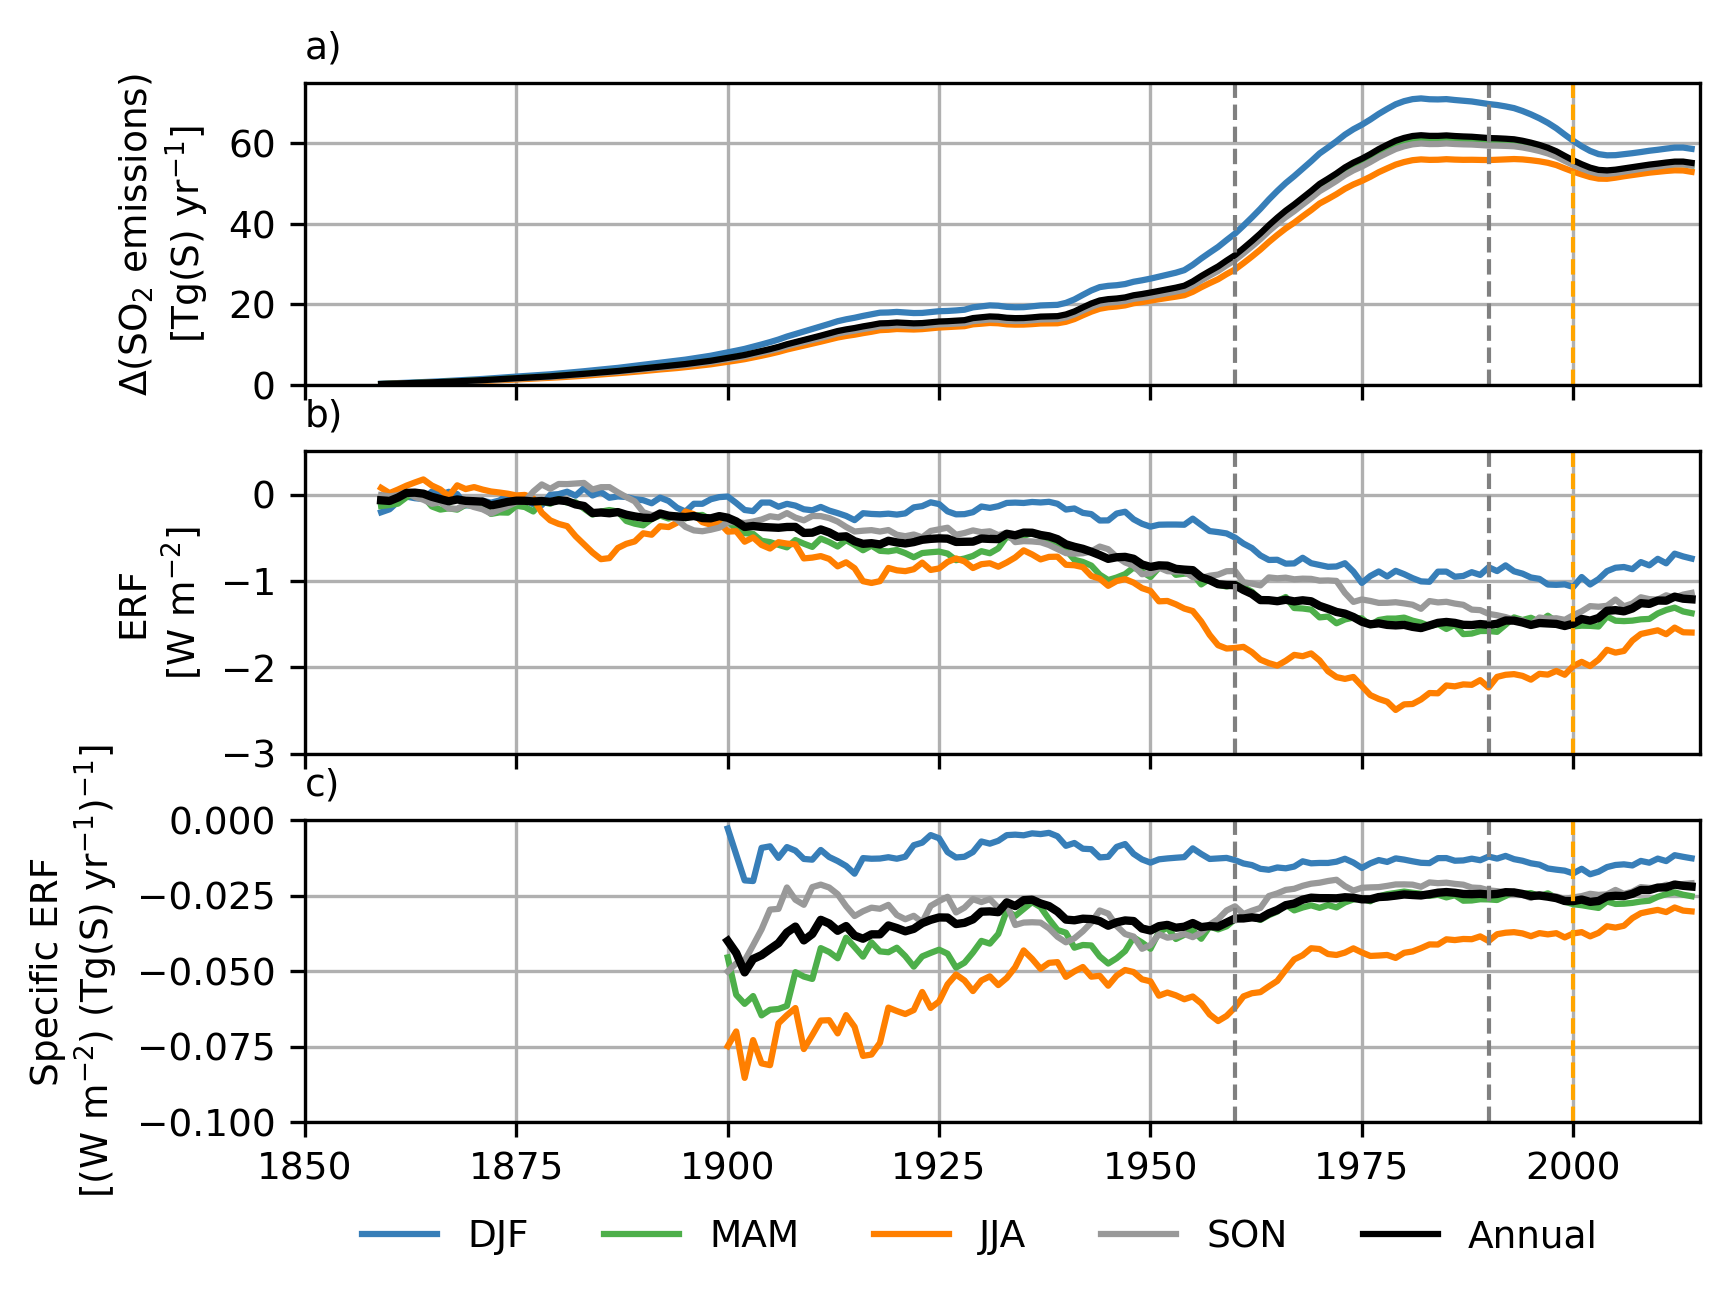
\includegraphics{Chapter4/Figs/seasonal_specific_erf.png}
    \caption[Specific ERF aggregated by seasons between 1900--2014]{Changes due to aerosol precursor emissions (i.e. \histsst{} minus \sstpiaer{}) of a) \ce{SO2} emissions, b) ERF and c) specific ERF (ERF per emitted \ce{SO2} aggregated by seasons with 10-year rolling average. Specific ERF is shown for 1900 onwards due to high noise from a small denominator. }
    \label{fig:ch4:specific-erf}
\end{figure}

Due to the nature of the available oxidants, \ce{SO2} emitted in summer has a stronger potential to impact the climate, as shown in Figure \ref{fig:ch4:specific-erf}. Specific ERF is the ERF per unit of \ce{SO2} emissions, following work by \citet{bellouinRegionalSeasonalRadiative2016}. During the pothole period, each teragram of sulfur emission contributes 4 times more cooling than the same amount emitted in winter (0.05 compared to 0.125 \unit{(W~m^{-2})~(Tg(S)~yr^{-1})^{-1})}. Specific ERF in autumn (SON) and winter (DJF) show less variation compared to summer, averaging at 0.125 \unit{(W~m^{-2})~(Tg(S)~yr^{-1})}. In contrast, specific ERF in Summer (JJA) decreases over time but is still at least 2 times greater than in winter.

% Note on Bellouin's 2016 work on specific RF. 
A previous study shows aerosol ERF is stronger in summer, especially when emissions are from Europe \citep{bellouinRegionalSeasonalRadiative2016}. Moreover, the specific RF from HadGEM3, a lower complexity model which predates UKESM1, is the most significant specific RF from \ce{SO2} emission in all models included in \citet{bellouinRegionalSeasonalRadiative2016}'s study. 


% there is substantial cooling from sulfate aerosol in summer, would it impact global mean surface air temperature?
It is now established that aerosols' impact on radiation is stronger in summer. Work done in this Chapter has contributed to understanding the observed behaviour in aerosol ERF.


\subsection{Surface air temperature anomaly and connection to aerosol radiative forcing}
\label{ch4:sec:seasonal-tas}

Aerosol-radiation interaction enhances the scattering of outgoing shortwave radiation, resulting in a negative ERF, which is shown to be stronger during the summer close to the emission region. There is evidence of aerosol impact on regional temperature change in diurnal time scale across seasons \citep[e.g. ][]{hanMechanismsSeasonalDifferences2020}. However, contrasting evidence exists on a global and longer temporal span, especially over the ocean. 

Aerosol's effect is local in the shorter and more regional scale. Anthropogenic aerosols indirectly increase surface temperature and decrease the diurnal temperature range in East Asia by reducing shortwave solar radiation and rising cloudiness and cloud liquid water \citep{huangImpactAerosolIndirect2006}. Aerosols reduce the global terrestrial mean diurnal temperature range by 0.47 K, with almost half the contribution coming from aerosols of anthropogenic origin \citep{chakrabortyLandCoverRegulates2019}. Aerosol causes changes in local air temperature, as observed in the urban heat island effect on a short time scale and regional scale \citep{hanMechanismsSeasonalDifferences2020}. % Explain urban heat island. 
Aerosols reduce urban heat island intensity in summer by cooling down surface temperature more strongly in urban areas than in rural areas but increase it in winter by weakening heat transport and expanding the planetary-boundary-layer stability.

While aerosol affects radiation budget locally and temporally on a short time scale, change in surface temperature does not have a simple localised or linear response to aerosol perturbation. Modelling studies show that sea surface temperature change due to aerosol shows a similar pattern to homogeneous forcing, i.e. greenhouse gases \citep{xieSimilarSpatialPatterns2013,kasoarSimilarSpatialPatterns2018}. Aerosols from different industrial regions (North America, Europe, East and South Asia) cause significant cooling across the hemisphere, showing a consistent spatial pattern of temperature changes regardless of the emission source \citep{kasoarSimilarSpatialPatterns2018, lewinschalLocalRemoteTemperature2019}.  


Acknowledging the multifaceted challenges, this section explores simulated surface air and sea temperature and compares them to observations to diagnose its possible connection to anomalous or pothole cooling observed between 1960 and 1980. 


\begin{figure}
    \centering
    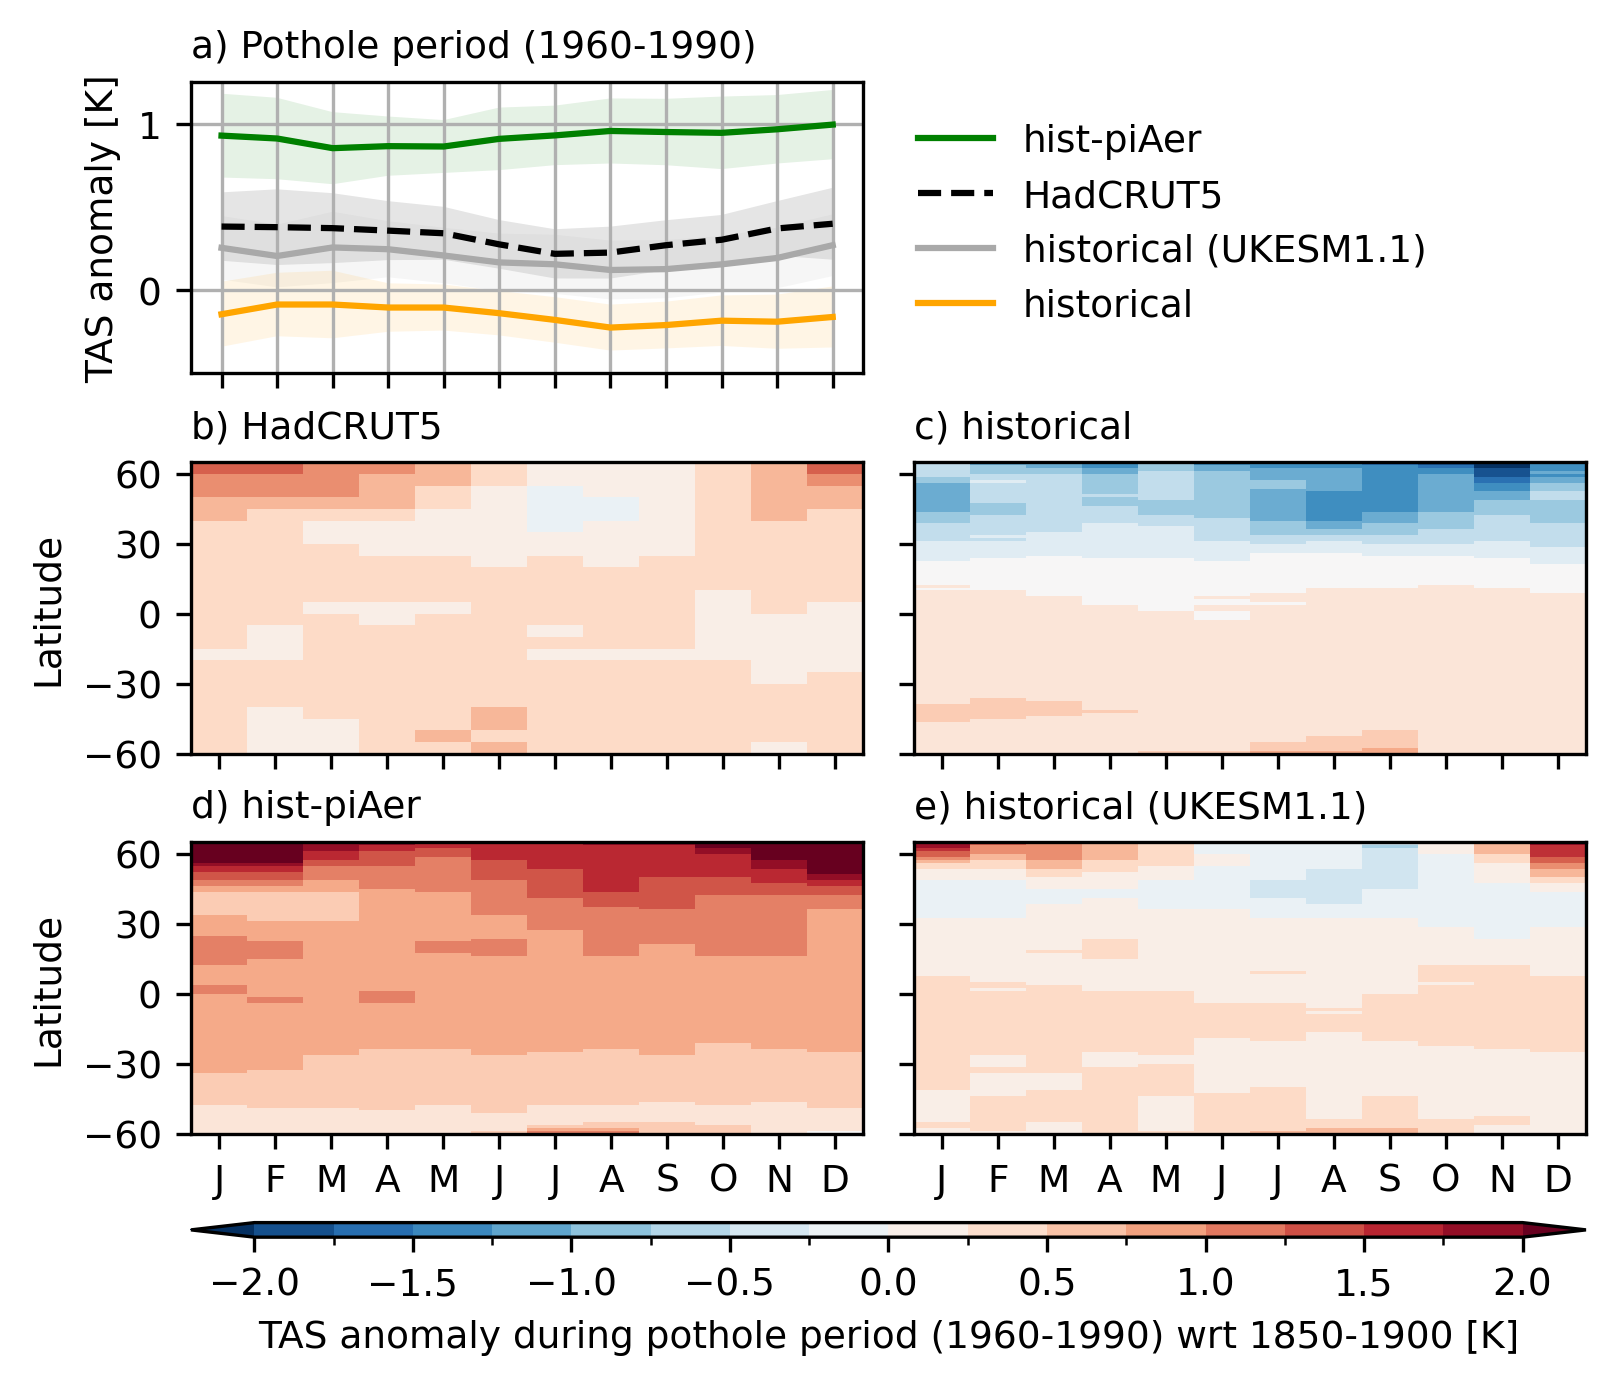
\includegraphics{Chapter4/Figs/TAS_anomaly_pothole.png}
    \caption[Surface air anomaly from HadCRUT5, UKESM1 and UKESM1.1 between 1960 and 1989]{a) mean surface air temperature anomaly between 1960--1989 with respect to 1850--1899 averaged over latitude 60\textdegree S and 65\textdegree N aggregated by month. b) surface air temperature anomaly from HadCRUT5 adjusted to 1850--1899. c-e) shows surface air temperature from UKESM1 c) \hist{} and d) \histpiaer{} simulation. d) is the same as c but from UKESM1.1. }
    \label{fig:ch4:seasonal-tas-anomaly-pothole}
\end{figure}

Figure \ref{fig:ch4:seasonal-tas-anomaly-pothole} shows the surface air temperature (TAS) from observation and model. HadCRUT5 shows a seasonal trend in TAS with the lowest temperature observed between June and September between Latitude 30 and 60 \textdegree N. The UKESM1 captures this trend but underestimates TAS globally. In contrast, the TAS anomaly in \histpiaer{} shows a different seasonal trend with the lowest anomaly in March. This shows that aerosol precursor controls the seasonal trend in TAS. 


\begin{figure}
    \centering
    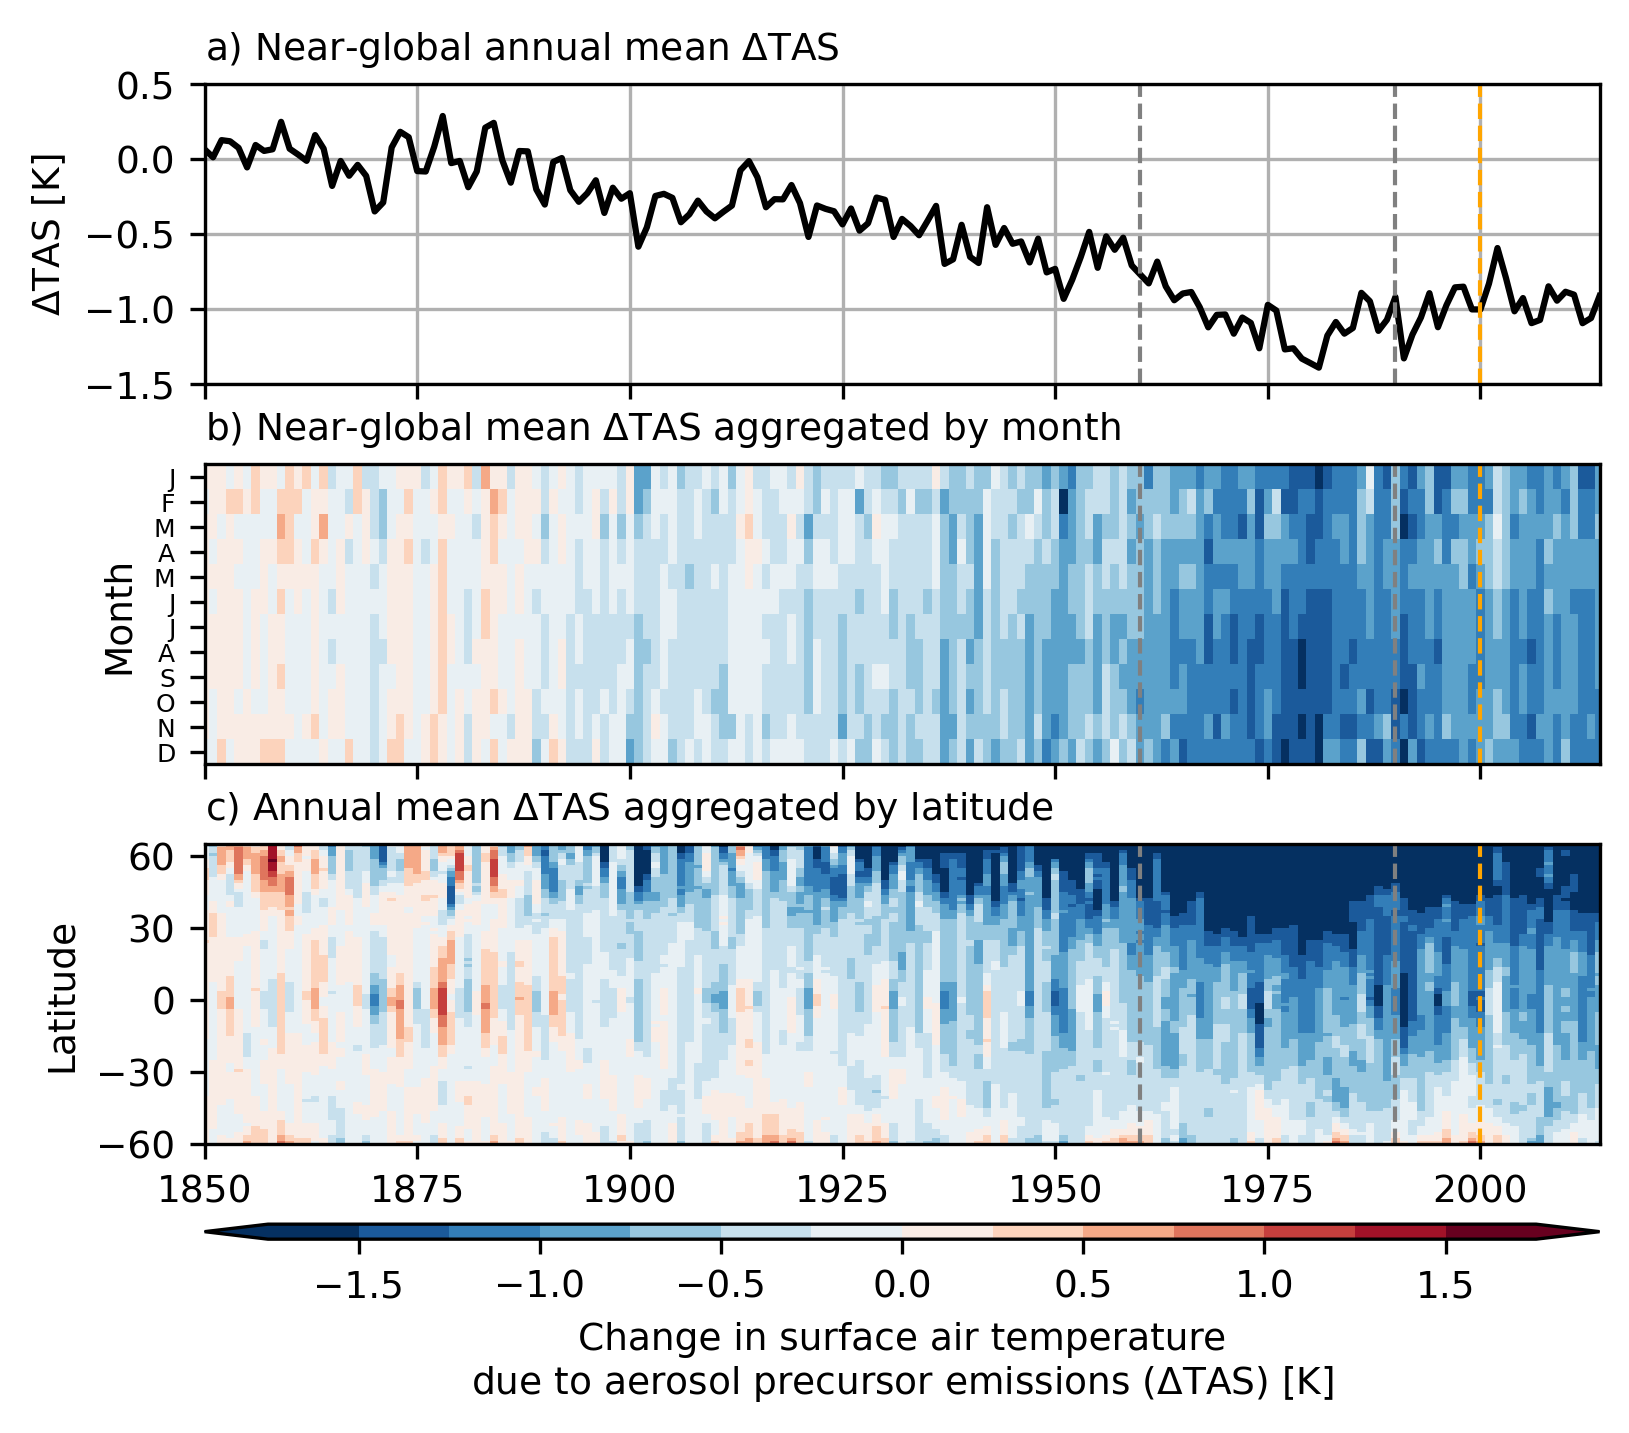
\includegraphics{Chapter4/Figs/tas_change_aerosols.png}
    \caption[Surface air temperature changes due to aerosol precursor emissions]{a) Annual mean surface air temperature changes due to aerosol precursor emissions averaged over latitude 60\textdegree S and 65\textdegree calculated from the difference between \hist{} and \histpiaer{}. b) Near-global mean surface air temperature aggregated by month and year. c) Near-global mean surface air temperature aggregated by month and latitude.}
    \label{fig:ch4:tas-change-aerosol}
\end{figure}

Figure \ref{fig:ch4:tas-change-aerosol} shows the change in near-global mean TAS due to aerosol precursor emissions. Aerosol cooling is strongest in the northern latitudes. At the maximum in the 1980s, aerosols cool down TAS by 1.5 K globally and more than 2 K in the northern hemisphere. After the pothole period, $\Delta$TAS slightly increases, and the Northern Hemisphere is not as cooled by aerosol. 


\begin{figure}
    \centering
    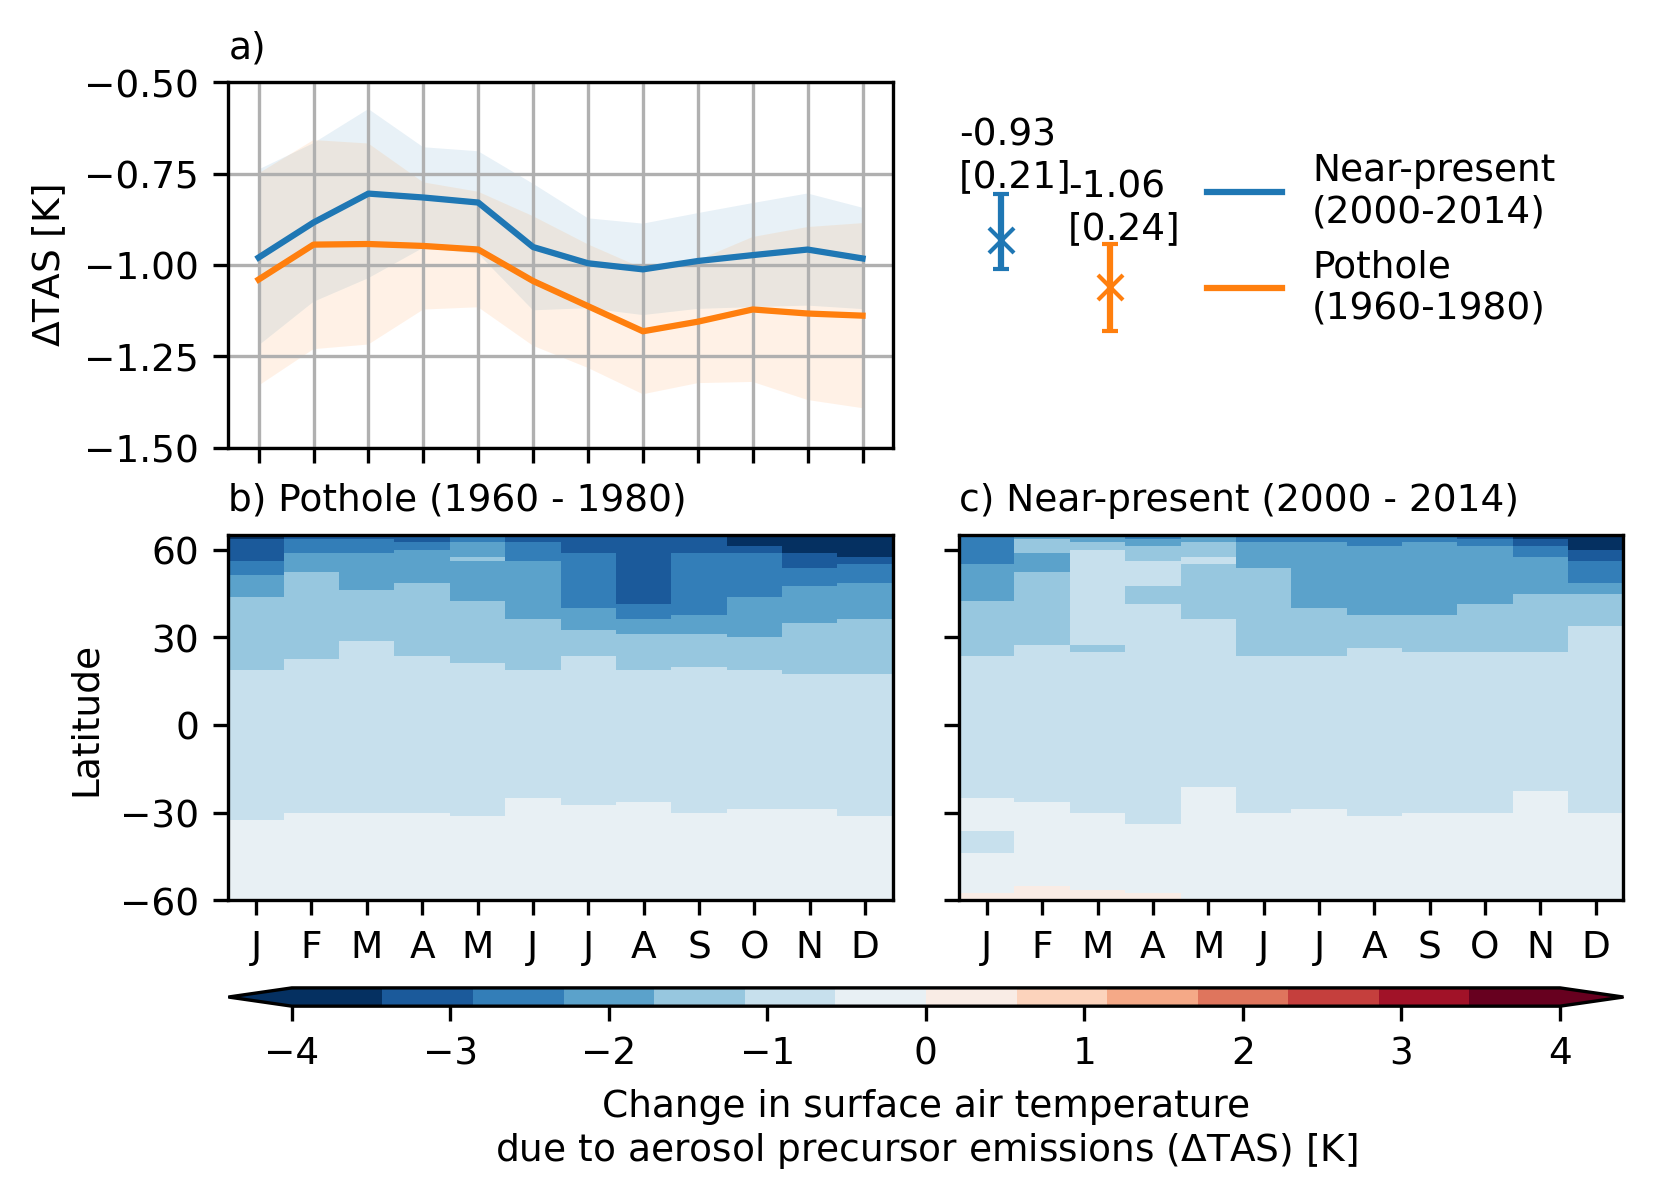
\includegraphics{Chapter4/Figs/tas_range.png}
    \caption[Change in surface air temperature due to aerosol precursor emissions for 1960--1989 and 2000-2014]{a) Near-global mean surface air temperature change due to aerosol precursor emissions (\hist{} minus \histpiaer{}) for the pothole and near-present period averaged over latitude 60\textdegree S and 65\textdegree N aggregated by month. $\Delta$TAS during b) pothole and c) near-present period aggregated by month and latitude. The notation next to a) shows the annual mean $\Delta$TAS and the range (maximum minus minimum) in square brackets.}
    \label{fig:ch4:tas-range}
\end{figure}

Figure \ref{fig:ch4:tas-range} shows the range of cooling between the maximum and minimum between two periods of interest: the pothole period (1960--1989) and near present (2000--2014). Aerosol reduces $\Delta$TAS, with the most significant impact in August in the Northern Hemisphere and the least in March and May. Both periods show a similar trend, but the range of $\Delta$TAS is greater during the pothole period (0.24 compared to 0.21 K)

\section{Conclusions}


% points: oxidants, oxidation, , importance of cloud fraction,  lifetime, cloud, ERF, specific ERF, correlation between SO2_OH and ERF, TAS
This chapter provides systematic view on the impact of \ce{SO2} oxidation in different seasons on aerosol and cloud formation, radiative effects and surface air temperature as simulated by UKESM1. Due to more photochemical production of oxidants in summer. UKESM1 simulates more aerosol particles in summer and shows strong ERF. The change in ERF per unit of \ce{SO2} emissions are reported, showing that \ce{SO2} emitted in summer has 2--4 times more potential to increase ERF. The model captures the seasonal trends in TAS anomaly (a more negative summer anomaly than winter and spring) compared to observation HadCRUT5. The model also shows a strong aerosol cooling during the pothole period compared to the present day, when the model performs well compared to HadCRUT5. While sulfate loading correlates with pothole cooling temperature \citep{zhangRoleAnthropogenicAerosols2021}, we suggest that aerosol loading in summer may contribute more significantly to anomalous cooling. 

Going forward, Other ESMs may benefit from a similar analysis proposed in this Chapter and assist in understanding the role of aerosol formation in this pothole problem. While \ce{SO2} emission in winter has a lower radiation effect and \citet{bellouinRegionalSeasonalRadiative2016} suggests that this could be used in controlled emissions where more \ce{SO2} can be emitted in winter due to lesser climatic impact, this work would like to suggest otherwise. \ce{SO2} emitted in winter has a longer lifetime, it is more likely to cause health impacts and should be considered.


% why do we overestimate cooling during the pothole period and not near present if this is due to seasonal bias? Is there something special about emitting SO2 over Europe/North America compared to China + India?
